\documentclass[12pt]{report}
\usepackage[a4paper,width=150mm,top=25mm,bottom=25mm]{geometry}
\usepackage{graphicx}
\usepackage[utf8]{inputenc}
\usepackage{alphabeta}
\usepackage[unicode]{hyperref}
\usepackage{textcomp}
\usepackage{listings}
\usepackage{xcolor}
\usepackage{microtype}
\usepackage{imakeidx}
\usepackage{eurosym}
\usepackage{appendix}
\makeindex[title=Ευρετήριο Όρων]

\definecolor{codegreen}{rgb}{0,0.6,0}
\definecolor{codegray}{rgb}{0.5,0.5,0.5}
\definecolor{codepurple}{rgb}{0.58,0,0.82}
\definecolor{backcolour}{rgb}{0.95,0.95,0.92}
\definecolor{mygreen}{rgb}{0,0.6,0}
\definecolor{mygray}{rgb}{0.5,0.5,0.5}
\definecolor{mymauve}{rgb}{0.58,0,0.82}

\lstset{ 
  commentstyle=\color{codegreen},
  keywordstyle=\color{magenta},
  numberstyle=\tiny\color{codegray},
  stringstyle=\color{codepurple},
  basicstyle=\footnotesize,        % the size of the fonts that are used for the code
  breakatwhitespace=false,         % sets if automatic breaks should only happen at whitespace
  breaklines=true,                 % sets automatic line breaking
  captionpos=b,                    % sets the caption-position to bottom
  % commentstyle=\color{mygreen},    % comment style
  deletekeywords={...},            % if you want to delete keywords from the given language
  escapeinside={\%*}{*)},          % if you want to add LaTeX within your code
  extendedchars=true,              % lets you use non-ASCII characters; for 8-bits encodings only, does not work with UTF-8
  %frame=single,                    % adds a frame around the code
  keepspaces=true,                 % keeps spaces in text, useful for keeping indentation of code (possibly needs columns=flexible)
  % keywordstyle=\color{blue},       % keyword style
  %language=Octave,                 % the language of the code
  morekeywords={*,...},            % if you want to add more keywords to the set
  numbers=left,                    % where to put the line-numbers; possible values are (none, left, right)
  numbersep=5pt,                   % how far the line-numbers are from the code
  % numberstyle=\tiny\color{mygray}, % the style that is used for the line-numbers
  rulecolor=\color{black},         % if not set, the frame-color may be changed on line-breaks within not-black text (e.g. comments (green here))
  showspaces=false,                % show spaces everywhere adding particular underscores; it overrides 'showstringspaces'
  showstringspaces=false,          % underline spaces within strings only
  showtabs=false,                  % show tabs within strings adding particular underscores
  stepnumber=1,                    % the step between two line-numbers. If it's 1, each line will be numbered
  % stringstyle=\color{mymauve},     % string literal style
  tabsize=2,                       % sets default tabsize to 2 spaces
  title=\lstname                   % show the filename of files included with \lstinputlisting; also try caption instead of title
}

\renewcommand{\figurename}{Εικόνα}
\newcommand*{\fullref}[1]{\hyperref[{#1}]{\ref*{#1} \nameref*{#1}}}
\newcommand*{\imgref}[1]{\hyperref[{#1}]{Εικόνα \ref*{#1}}}
\newcommand*{\sucite}[1]{\textsuperscript{\cite{#1}}}

 
\graphicspath{ {images/} }

\title{
    {Κατασκευή Έξυπνης, Τηλεχειριζόμενης Κλειδαριάς Θυροτηλεφώνου με χρήση Τεχνολογιών Αιχμής }\\
    {\large Πανεπιστήμιο Πειραιώς}
}
\author{Κυριάκος Δ. Γιαννάκης}
\date{Day Τεστ Year}

\begin{document}
    \maketitle
    
    \begin{abstract}
        TODO
    \end{abstract}
    
    \tableofcontents
    
    \chapter{Εισαγωγή}
    Στον σημερινό κόσμο, οι τεχνολογικές μας ανάγκες γίνονται ολοένα και πιο πολύπλοκες. Κάθε μέρα βγαίνουν στην επιφάνεια νέες τεχνολογικές διευκολύνσεις για τον άνθρωπο, σκοπός των οποίων είναι να κάνουν την διαβίωσή του πιο "έξυπνη", δίνοντάς του τον μέγιστο έλεγχο σε κάθε σημείο της ζωής του. Με την άνθιση του internet of things, γίνεται εύκολη η διασύνδεση πολλών συσκευών (από την μικρότερη ως την μεγαλύτερη), με σκοπό τον έλεγχό τους και την άντληση δεδομένων από αυτές, απομακρυσμένα.

\textbf{Σκοπός της παρούσας πτυχιακής εργασίας είναι να περιγράψει την πλήρη διαδικασία του σχεδιασμού και υλοποίησης ενός συστήματος ελέγχου κλειδαριάς σπιτιού/γραφείου, γνωστό ως PiLock.}

Η εφαρμογή υλοποιήθηκε, στο μεγαλύτερο μέρος της, χρησιμοποιόντας λογισμικό τελευταίας τεχνολογίας, πράγμα που μας εγγυάται την μέγιστη ευελιξία όσων αφορά την ανάπτυξη, πράγμα που ισοδυναμεί με μέγιστη ταχύτητα ανάπτυξης και αυξημένη ασφάλεια. %Αξίζει σε αυτό το σημείο να αναφέρουμε οτι δεν πρέπει να μπερδεύουμε το λογισμικό τελευταίας τεχνολογίας με το Bleeding Edge Software (Λογισμικό τεχνολογίας αιχμής).

\section{Internet of Things}
	Ο όρος "\idxa{Internet of Things}" (IoT) χρησιμοποιήθηκε πρώτη φορά από τον Kevin Ashton το 1999 σε μία παρουσίασή του στην Procter \& Gamble (P\&G) \cite{iotterm}. Ο όρος επινοήθηκε προκειμένου να μπορεί να τονιστεί η δύναμη της (τότε) δημοφιλούς ιδέας της χρήσης της τεχνολογίας RFID σε συστήματα εφοδιαστικών αλυσίδων εταιριών για παρακολούθηση εμπορευμάτων. Πλέον, ο όρος Internet of Things χρησιμοποιείται προκειμένου να χαρακτηριστούν συσκευές (μικρές ή μεγάλες) με δυνατότητα σύνδεσης στο Internet. Κάποια παραδείγματα είναι τα αυτοκίνητα με ενσωματομένους αισθητήρες, τα έξυπνα σπίτια (τα οποία αποτελούνται από μια πληθώρα έξυπνων συσκευών), καθώς επίσης και συγκεκριμένες συσκευές παρακολούθησης υγείας (όπως πχ. συσκευές παρακολούθησης καρδιακού ρυθμού) με δυνατότητα σύνδεσης στο διαδίκτυο.

	Οι δυνατότητες που έχουν οι συγκεκριμένες συσκευές τις καθιστούν ικανές για σύνδεση στο internet, και κατ'επέκταση, αυξάνουν σημαντικά τις λειτουργίες τους, προσδίδοντας μεγαλύτερο έλεγχο στον χρήστη. %Check it...

\section{Αυτοματισμοί Σπιτιού - Home Automation}
	Μία από τις πιο σημαντικές υποκατηγορίες των συσκευών Internet of Things είναι οι \textbf{συσκευές αυτοματισμού σπιτιών (Home Automation Devices, \idxa{Domotics} \cite{domotics} )}. Οι συσκευές αυτές δίνουν στον χρήστη τους την δυνατότητα να διαχειριστεί διάφορες συσκευές του σπιτιού/γραφείου του. Οι συσκευές αυτές μπορεί να είναι συσκευές κλιματισμού, φωτισμός, συστήματα διασκέδασης (Home Theaters, Music Stereos, κτλ...), καθώς επίσης και συστήματα συναγερμού ή και διαχείρησης πρόσβασης. Το PiLock ανήκει στην τελευταία αυτή κατηγορία.

	Συνήθως, οι συσκευές αυτές συνδέονται σε ένα κεντρικό κόμβο (Hub) προκειμένου να ελέγχονται όλες από ένα μοναδικό σημείο. Η δυνατότητα αυτή μπορεί να προστεθεί σε μία επόμενη έκδοση του PiLock (βλ. \fullref{ch:future_expansion}). Την παρούσα χρονική στιγμή, δεν υπάρχει αυτή η δυνατότητα.

\section{Σκοπός του PiLock}
	Το PiLock ανήκει στην κατηγορία συσκευών \textbf{"έξυπνου σπιτιού" (Smart Home)}. Σκοπός του είναι να παρέχει στον χρήστη την δυνατότητα να ξεκλειδώνει εύκολα την εξώπορτα/πόρτα του σπιτιού/γραφείου του, μέσω του SmartPhone ή του SmartWatch του, όλα αυτά χρησιμοποιόντας το ασφαλέστερο δυνατόν περιβάλλον, προκειμένου να αποφευχθεί εισβολή τρίτων.

	Μέσω του \textbf{\idxa{PiLock Administration Control Panel (PiLock AdminCP)}}, δίνουμε στον διαχειριστή του συστήματος ένα εύχρηστο περιβάλλον διαχείρησης από το οποίο μπορεί εύκολα και γρήγορα να διαχειρίζεται το PiLock. Δίνεται δυνατότητα διαχείρησης των \textbf{εξουσιοδοτημένων χρηστών (χρήστες που μπορούν να ξεκλειδώσουν την πόρτα μέσω του PiLock)}, δυνατότητα λήψης ζωτικής σημασίας πληροφοριών για το σύστημα, καθώς επίσης και της δυνατότητας ξεκλειδώματος της πόρτας απευθείας μέσω του πίνακα διαχείρησης, χωρίς να χρειάζεται να γίνει χρήση της εφαρμογής (AdminCP Unlock).

	Ένας από τους στόχους, κατά τον σχεδιασμό του PiLock ήταν η διατήρηση του κόστους στο χαμηλότερο δυνατόν. Για να επιτευχθεί ο στόχος αυτός, χρησιμοποιήθηκε αυστηρά δωρεάν λογισμικό ανοικτού κώδικα, καθώς επίσης και εξαρτήματα εύκολα προσκομίσιμα (βλ. \fullref{ch:structure}).

\section{Έρευνα αγοράς - Καινοτομία του PiLock}
	Έπειτα από έρευνα που έγινε πάνω σε ήδη υπάρχοντες μηχανισμούς ξεκλειδώματος μέσω Raspberry Pi βρέθηκε οτι το PiLock είναι το πρώτο σύστημα ξεκλειδώματος που συνδέεται απευθείας πάνω στο κύκλωμα του θυροτηλεφώνου και χειρίζεται την κλειδαριά. 

	\subsection{Μη Εμπορικές/DIY Εφαρμογές}
		Ανάμεσα στα συστήματα που βρέθηκαν, υπάρχει ένα σύστημα που συνδέεται απευθείας επάνω στην κλειδαριά της πόρτας, αλλά σε κλειδαριά διαφορετικού τύπου από ό,τι χρησιμοποιείται στις περισσότερες πολυκατοικίες στην Ελλάδα, δημιουργημένο από έναν YouTuber γνωστό ως Hacker Shack\footnote{https://bit.ly/2LGTSJd}. Το συγκεκριμένο σύστημα χρησιμοποιείται σε κλειδαριές τύπου Deadbolt, αντί για κλειδαριές τύπου Electric Strike (βλ. \fullref{ch:unlock_mechanism}).

		Υπάρχει ένα παρόμοιο, επίσης, σύστημα με την ονομασία "Pi-Lock", κατασκευασμένο από τον Paolo Bernasconi\footnote{http://www.pi-lock.com/}, το οποίο χρησιμοποιεί Raspberry Pi αλλά προσφέρει λειτουργικότητα ξεκλειδώματος μέσω RFID, έναντι των ξεκλειδωμάτων μέσω Android, τα οποία προσφέρει το PiLock.

	\subsection{Εμπορικές Εφαρμογές}
		Έπειτα από έρευνα που έγινε στις υπάρχουσες εμπορικές εφαρμογές έξυπνης κλειδαριάς, που μπορεί να προμηθευτεί ο οποιοσδήποτε, εξάγεται το συμπέρασμα οτι η πλειονότητα αυτών των εφαρμογών (παίρνοντας ως δείγμα το άρθρο με τις καλύτερες έξυπνες κλειδαριές του 2018, από το PC Magazine)\sucite{best_sl} απαιτούν να ξοδευτεί αρκετά μεγάλο χρηματικό ποσό, σε σύγκριση με το ποσό που πρέπει να ξοδευτεί για να αγοραστούν τα εξαρτήματα του PiLock, και συνήθως απαιτούν αντικατάσταση της ήδη υπάρχουσας κλειδαριάς, το οποίο σημαίνει οτι μπορεί να χρειαστούν παραπάνω χρήματα για την πρόσληψη τεχνικού που θα πραγματοποιήσει την αντικατάσταση.

	\subsection{Διαφορές του PiLock με τις ήδη υπάρχουσες εφαρμογές}
		Το PiLock, εκτός του οτι είναι πολύ φθηνότερο σε σχέση με τις ήδη υπάρχουσες εμπορικές εφαρμογές που κυκλοφορούν, είναι πολύ ευκολότερο στην εγκατάσταση και μπορεί να εγκατασταθεί απευθείας στο ήδη υπάρχον σύστημα θυροτηλεφώνου που έχουν οι πολυκατοικίες, χωρίς να χρειαστεί να γίνει αλλαγή κλειδαριάς. Πέραν αυτού, με την προσθήκη συμβατότητας με Android Wear που έγινε στην έκδοση \verb|0.3.0|, είναι μία από τις πρώτες εφαρμογές παγκοσμίως που υποστηρίζουν ξεκλείδωμα πόρτας μέσω Smartwatch.

    \chapter{Δομή του PiLock}
    \label{ch:structure}
Το PiLock χρησιμοποιεί \idxa{Αρχιτεκτονική Πελάτη-Εξυπηρετητή (Client-Server Architecture)}.
% To PiLock αποτελείται από 2 κύρια μέρη: Τον εξυπηρετητή (Server) και τον πελάτη (Client).

\section{Σύντομη Περιγραφή Λογισμικού Εξυπηρετητή - PiLock Server}
	Ο εξυπηρετητής αποτελείται από το Hardware που χρειάζεται προκειμένου να λειτουργήσει το PiLock, καθώς επίσης και το αντίστοιχο λογισμικό υπεύθυνο για την διαχείρηση του συστήματος ξεκλειδώματος. Πιο συγκεκριμένα, το λογισμικό είναι υπεύθυνο για:
	\begin{itemize}
		\item Την διαχείριση του Hardware υπεύθυνου για την λειτουργία του μηχανισμού ξεκλειδώματος.
		\item Την αυθεντικοποίηση των ήδη υπάρχοντων χρηστών.
		\item Την δημιουργία νέων χρηστών, ικανών για αυθεντικοποίηση (εξουσιοδοτημένοι χρήστες).
		\item Την τήρηση ιστορικού αυθεντικοποιήσεων (επιτυχών ή μή).
	\end{itemize}
	Το λογισμικό του εξυπηρετητή αναλύεται πλήρως στην ενότητα \ref{ch:server}. %TODO FIX IT

\section{Σύντομη Περιγραφή Λογισμικού Πελάτη - PiLock Client}
	\label{sec:pilock_client_overview}
	Η πλευρά του πελάτη αποτελείται από την εφαρμογή του PiLock, σχεδιασμένη για κινητά που τρέχουν Android, καθώς επίσης και από την εφαρμογή σχεδιασμένη για Android Wear Smartwatches.

	Πιο συγκεκριμένα, οι εφαρμογές στο πεδίο του πελάτη είναι υπεύθυνες για:

	\begin{itemize}
		\item Σύνδεση στην πλατφόρμα του PiLock\textsuperscript{*}.
		\item Αποστολή αιτημάτων ξεκλειδώματος.
		\item Αποστολή αιτημάτων αλλαγής PIN\textsuperscript{*}.
	\end{itemize}
	{\footnotesize Οι δυνατότητες που είναι σημειωμένες με τον αστερίσκο (*) είναι διαθέσιμες αποκλειστικά στην εφαρμογή για κινητά (mobile app) και όχι στην εφαρμογή για Android Wear.}

\section{Υλικό - Hardware}
	\label{sec:hardw}
	Όπως αναφέρθηκε και στην εισαγωγή, ένας εκ των στόχων από τις πρώτες μέρες του σχεδιασμού του PiLock ήταν να υλοποιηθεί το Project με όσο το δυνατόν λιγότερο κόστος. Προκειμένου αυτό να είναι εφικτό, χρησιμοποιήσαμε υλικό εύκολα προσκομίσιμο και, όπου ήταν δυνατόν, Open Source Hardware.

	\subsection{Raspberry Pi Zero W}
		"Εγκέφαλος" όλης της κατασκευής είναι το \idxa{Raspberry Pi Zero W (RPi Zero W)}, ένας υπολογιστής μοναδικής πλακέτας (Single Board). Σχεδιάζεται από το Raspberry Pi Foundation στην Αγγλία και η κυκλοφορία του ξεκίνησε τον Φεβρουάριο του 2017. Σκοπός του RPi Zero W είναι να συμπληρώσει το προηγούμενο μοντέλο, το Raspberry Pi Zero, φέρνοντας δυνατότητες συνδεσιμότητας WiFi 802.11n και BlueTooth 4.0 χωρίς Hardware κάποιου τρίτου (μέχρι προτίστως έπρεπε να χρησιμοποιηθεί κάποιο WiFi ή BlueTooth Dongle προκειμένου να υπάρξει αυτή η συνδεσιμότητα) \sucite{rpizw}.

		\begin{figure}[h]
			\centering
				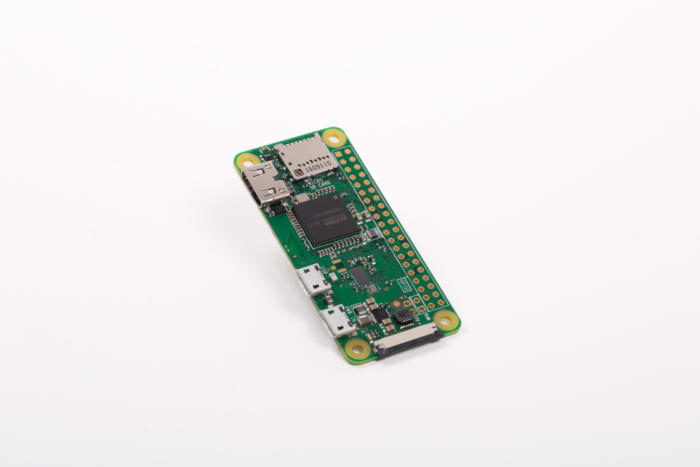
\includegraphics[width=\textwidth,height=\textheight,keepaspectratio]{rpizerow.jpg}
			\caption{Το Raspberry Pi Zero W.}
		\end{figure}

		Στην "καρδιά" του RPi Zero W υπάρχει ένας Broadcom BCM2835, 32-bit επεξεργαστής αρχιτεκτονικής ARMv6, χρονισμένος στο 1Ghz. Για μνήμη τυχαίας προσπέλασης χρησιμοποιούνται 512MB Low Power Double Data Rate 2 (LPDDR2) RAM. Πανω στο RPi Zero W δεν υπάρχει αποθηκευτικός χώρος, οπότε χρησιμοποιείται μια κάρτα MicroSD. 

		Ένα από τα σημαντικότερα σημεία ενός RPi Zero W είναι οι \textbf{\idxa{Δέκτες Εισόδου/Εξόδου Γενικού Σκοπού (General Purpose Input/Output, GPIO)}}. Μέσω αυτών καθίσταται δυνατόν να συνδεθεί το RPi με μια πληθώρα εξωτερικών αισθητήρων, διακοπτών (Relay Modules), πλακετών επέκτασης (γνωστά ως HATs), και εξαρτημάτων και να αντλήσει πληροφορίες από αυτά ή να τα ελέγξει.

	\subsection{Relay Module}
		\label{sub:relay}
		Προκειμένου να μπορέσει να συνδεθεί το RPi με το ήδη υπάρχον σύστημα ξεκλειδώματος, χρειάζεται ένας ηλεκτρονικά ελεγχόμενος διακόπτης. Θα χρησιμοποιηθεί ένα \textbf{\idxa{Relay Module}}. Τα Relay Modules χρησιμοποιούνται ως διακόπτες προκειμένου να ελέγχονται κυκλώματα μέσω υπολογιστών/μικροελεγκτών, οι οποίοι λειτουργούν μέσω σημάτων μικρής ισχύος\sucite{relay_purpose}.

		Τα Relay Modules κυκλοφορούν σε πολλούς τύπους. Οι τρείς κυριότεροι είναι:
		\begin{itemize}
			\item 5V Compatible, Active Low. 
			\item 5V/3.3V Compatible, Active High.
			\item 3.3V Compatible Active High/Low.
		\end{itemize}

		Το Raspberry Pi, εφόσον λειτουργεί σε λογική 3.3V, είναι συμβατό με τους 2 τελευτέους τύπους. Αν θελήσει ο χρήστης να χρησιμοποιήσει ένα Relay Module που να λειτουργεί σε λογική 5V και είναι Active Low, θα χρειαστεί να χρησιμοποιήσει ένα Arduino.

		Τα Relay Modules αποτελούνται από ένα Relay τύπου SRD, έναν φωτοσυζευκτή (Optocoupler), ευθύνη του οποίου είναι να απομονώνει το κύκλωμα ωστε να μην επηρρεάσει η υψηλή τάση (σε περίπτωση που χρησιμοποιείται από το σύστημα ξεκλειδώματος του κτηρίου) το υπόλοιπο κύκλωμα, ένα Transistor και μια δίοδο. Είναι σημαντικό να τονιστεί οτι καλό είναι να μην χρησιμοποιούνται Relay Modules που δεν φέρουν Φωτοσυζευκτή, καθώς μπορεί, σε περίπτωση που χρησιμοποιείται υψηλή τάση, να επηρρεαστεί, ακόμα και να καεί, το Raspberry Pi ή/και το Arduino. %TODO Needs citation.

		%TODO Add Figure...

	\subsection{Arduino UNO}
		Το \textbf{\idxa{Arduino UNO}} είναι ένας Ανοικτού-Κώδικα (Open Source) μικροελεγκτής σχεδιασμένος από την \href{https://www.arduino.cc/}{Arduino.cc}. Είναι βασισμένος πάνω στον ATmega328 microcontroller της Atmel. Μπορεί να χρησιμοποιηθεί προκειμένου να χειρίζεται και να αντλεί πληροφορίες από διάφορα εξαρτήματα στον φυσικό κόσμο. Εξαιτίας της μεγάλης ευελιξίας του έχει γίνει μία από τις δημοφιλέστερες επιλογές για κατασκευαστές, οι οποίοι το χρησιμοποιούν για μια τεράστια γκάμα εφαρμογών\sucite{arduino_definition}.

		To Arduino UNO μπορεί να χρησιμοποιηθεί σε περίπτωση που δεν χρησιμοποιηθεί κάποιο Relay συμβατό με το Raspberry Pi (βλ. \fullref{sub:relay}), αρκεί να λειτουργεί με λογική 5V.

		Μπορεί, έναντι του Arduino UNO, και προκειμένου να εξοικονομηθεί χώρος, να χρησιμοποιηθεί ένα \idxa{Arduino Nano}, το οποίο έχει όλες τις αναγκαίες λειτουργίες για την λειτουργία του PiLock.

		Ρεύμα για την λειτουργία του Arduino παρέχεται από την θύρα Micro USB του RPi, και μέσω αυτού δίνεται ρεύμα και σε οποιοδήποτε Relay Module συνδεθεί με αυτό. Για να γίνει αποστολή δεδομένων από το RPi στο Arduino χρησιμοποιείται η \idxa{Σειριακή Θύρα (Serial Port)} του Arduino.

		\begin{figure}[h]
			\centering
				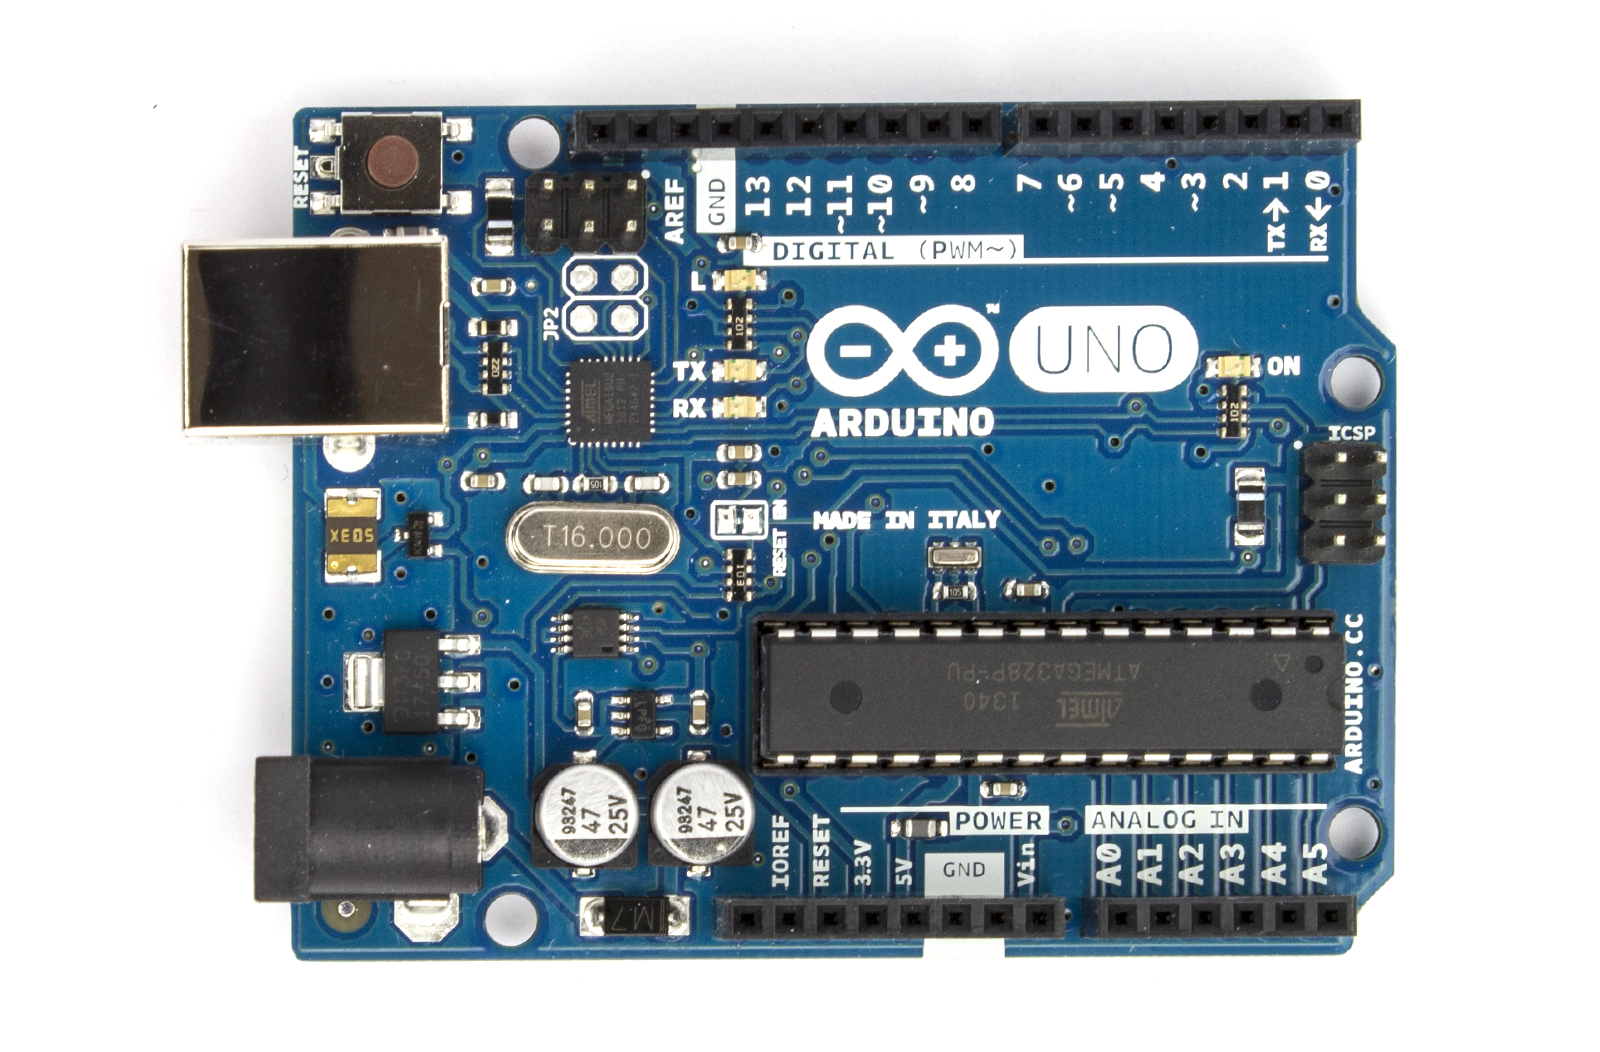
\includegraphics[width=0.5\textwidth,height=0.5\textheight,keepaspectratio]{arduino_uno.jpg}
			\caption{Arduino Uno Rev3, oomlout (2015), Flickr, CC BY-SA 2.0}
		\end{figure}

	\subsection{Λοιπό Hardware}
		Προκειμένου να συναρμολογηθεί η κατασκευή θα χρειαστουν κάποια συγκεκριμένα υλικά, εύκολα προμηθεύσιμα από διάφορα μαγαζιά πώλησης υλικών για ηλεκτρονικές κατασκευές.

		\subsubsection{Κουτί Κατασκευής (Project Box):}
			Ανάλογα τον τρόπο σύνδεσης που θα χρησιμοποιηθεί για την σύνδεση του RPi με το Relay Module, και ανάλογα με το αν είναι συμβατό το Relay Module με λογική 3.3V, θα χρειαστεί διαφορετικό μέγεθος κουτιού κατασκευής. 

			\paragraph{Σύνδεση χωρίς χρήση Arduino:}
				Ο προεπιλεγμένος τρόπος σύνδεσης, από την έκδοση \verb|0.3.1| και μετά είναι χωρίς την χρήση Arduino. Έπειτα από μετρήσεις βρέθηκε οτι το κατάλληλο κουτί κατασκευής έχει διαστάσεις 10cm x 10cm.
			\paragraph{Σύνδεση με Arduino:}
				Εφόσον χρειάζεται να γίνει σύνδεση με Arduino (προκειμένου να μπορεί να λειτουργήσει το Relay Module), έπειτα απο μετρήσεις βρέθηκε οτι το κατάλληλο κουτί κατασκευής έχει διαστάσεις 18cm x 14cm.

		\subsubsection{Καλώδια σύνδεσης:}
			Για να συνδεθεί το Relay Module με το RPi (ή το Arduino), θα χρειαστούν κάποια συγκεκριμένα καλώδια σύνδεσης γνωστά ως Jumper Wires. Τα Jumper Wires κάνουν εύκολη την σύνδεση σε διάφορα εξαρτήματα καθώς δεν χρειάζονται συγκόλληση \textsuperscript{\cite{jumper_wires}}.

		 	\paragraph{Σύνδεση χωρίς χρήση Arduino:}
		 		Θα χρειαστούν τουλάχιστον 3 Jumper Wires Female-Male (ή Female-Female, σε περίπτωση χρήσης του Male Header).
		 	\paragraph{Σύνδεση με Arduino:}
		 		\label{par:ard_conn}
		 		Θα χρειαστούν τουλάχιστον 3 Jumer Wires Female-Male, αν χρησιμοποιηθεί Arduino UNO ή 3 τουλάχιστον καλώδια Female-Female, αν χρησιμοποιηθεί Arduino Nano. Επίσης, θα χρειαστεί ένα καλώδιο Micro USB-B to USB-A (\idxa{OTG Cable}) και ένα καλώδιο USB-A to USB-B αν χρησιμοποιηθεί ένα Arduino UNO ή ένα καλώδιο USB-A to Micro USB-B σε περίπτωση χρήσης Arduino Nano.

		 	\begin{figure}[h]
			\centering
				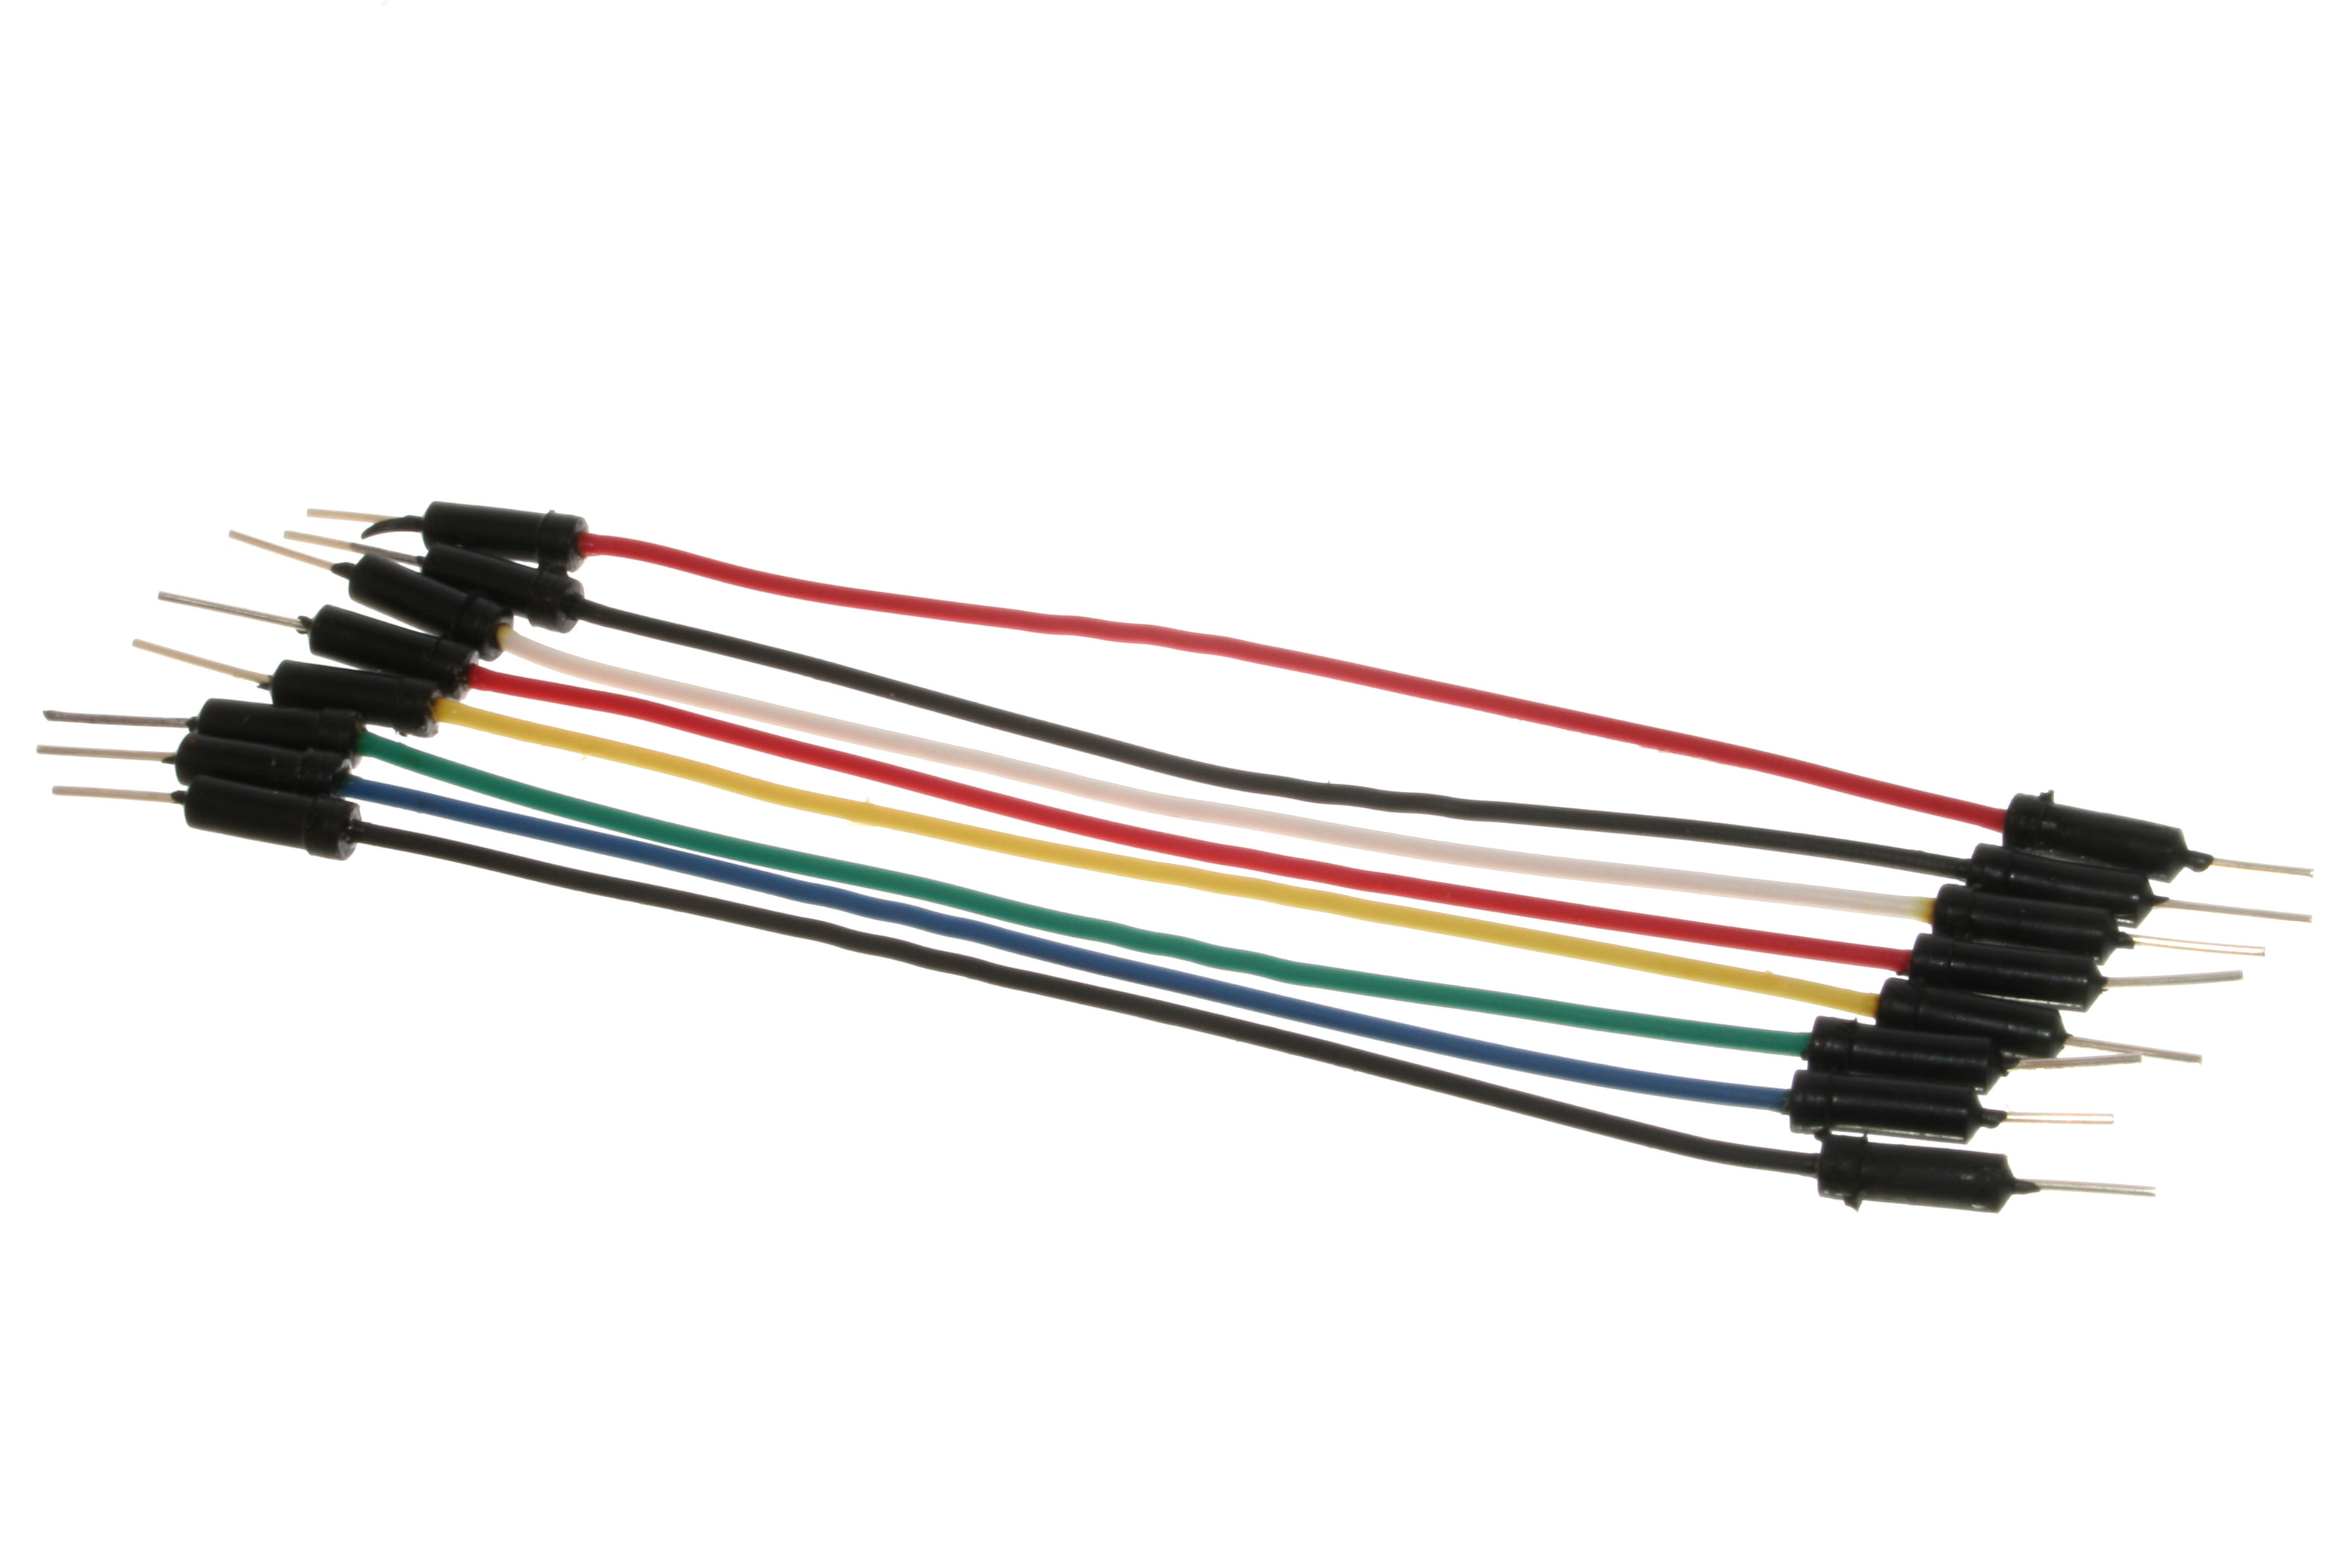
\includegraphics[width=0.5\textwidth,height=0.5\textheight,keepaspectratio]{jumper_wires.jpg}
				\caption{Jumper Wires (Male-Male), oomlout (2009), Flickr, CC BY-SA 2.0}
			\end{figure}

\section{Κόστος Κατασκευής του PiLock}
	Με βάση την παραπάνω λίστα υλικών που θα χρησιμοποιηθούν για την συναρμολόγηση του PiLock, μπορεί να εξαχθεί ένα τελικό κόστος για την προμήθεια των υλικών αυτών. Να σημειωθεί οτι η εξαγωγή των τιμών αυτών έγινε έπειτα από έρευνα σε διάφορα ηλεκτρονικά μαγαζιά, είτε Ελληνικά, είτε του εξωτερικού, προκειμένου να κρατηθεί σε όσο το δυνατόν χαμηλότερα πλαίσια το τελικό κόστος.

	\begin{center}
	\begin{tabular}{||c c||}
		\hline
		Υλικό & Κόστος \\ [0.5ex] 
		\hline\hline
		Raspberry Pi Zero W\textsuperscript{*} & 17.46\euro \\
		Project Box (18x14) & 4.90\euro \\
		Relay Module & 2.75\euro \\
		Arduino Uno (Κλώνος) & 5.00\euro \\
		Καλώδια & 0.70\euro \\
		\hline\hline
		Τελικό Κόστος: & 30.81\euro \\
		\hline
	\end{tabular}
	\end{center}

	{\footnotesize *: Συμπεριλαμβάνεται Καλώδιο OTG, GPIO Headers}

	Να σημειωθεί οτι, όπως είναι αντιληπτό, στο παραπάνω κόστος συμπεριλαμβάνεται και το Arduino. Εάν αγοραστεί συμβατό με το Raspberry Pi, Relay Module, το κόστος κατεβαίνει στα 23,81\euro, καθώς δεν απαιτείται η χρήση Arduino και, κατ'επέκταση, απαιτείται και μικρότερο Project Box.

    \chapter{Συστήματα Ελέγχου Πρόσβασης Πολυκατοικιών/Σπιτιών}
    \label{ch:unlock_mechanism}
Πριν να εξηγήσουμε τον τρόπο κατασκευής και λειτουργίας του PiLock, είναι αναγκαίο να αναφερθούμε στον τρόπο λειτουργίας των περισσότερων κλειδαριών σπιτιών, πολυκατοικιών ή και γραφείων.

Το σύστημα ξεκλειδώματος που χρησιμοποιείται στις περισσότερες κατοικίες αποτελείται από 2 εντελός ξεχωριστά και ανεξάρτητα συστήματα: Το σύστημα του θυροτηλεφώνου, δηλαδή το σύστημα μέσω του οποίου γίνεται η αναγνώριση του επισκέπτη (μέσω φωνής ή/και εικόνας), και το σύστημα ενεργοποίησης της κλειδαριάς. Στην παρούσα διατριβή θα αναφερθούμε αποκλειστικά στο δεύτερο σύστημα.

Οι ηλεκτρικές κλειδαριές που χρησιμοποιούνται σε πολυκατοικίες συνήθως αποτελούνται από ένα μάνταλο το οποίο, όταν το σύστημα ενεργοποιηθεί μέσω ρεύματος, απελευθερώνεται με αποτέλεσμα να μπορεί ελεύθερα η πόρτα να ανοίξει.

\begin{figure}[h]
	\centering
		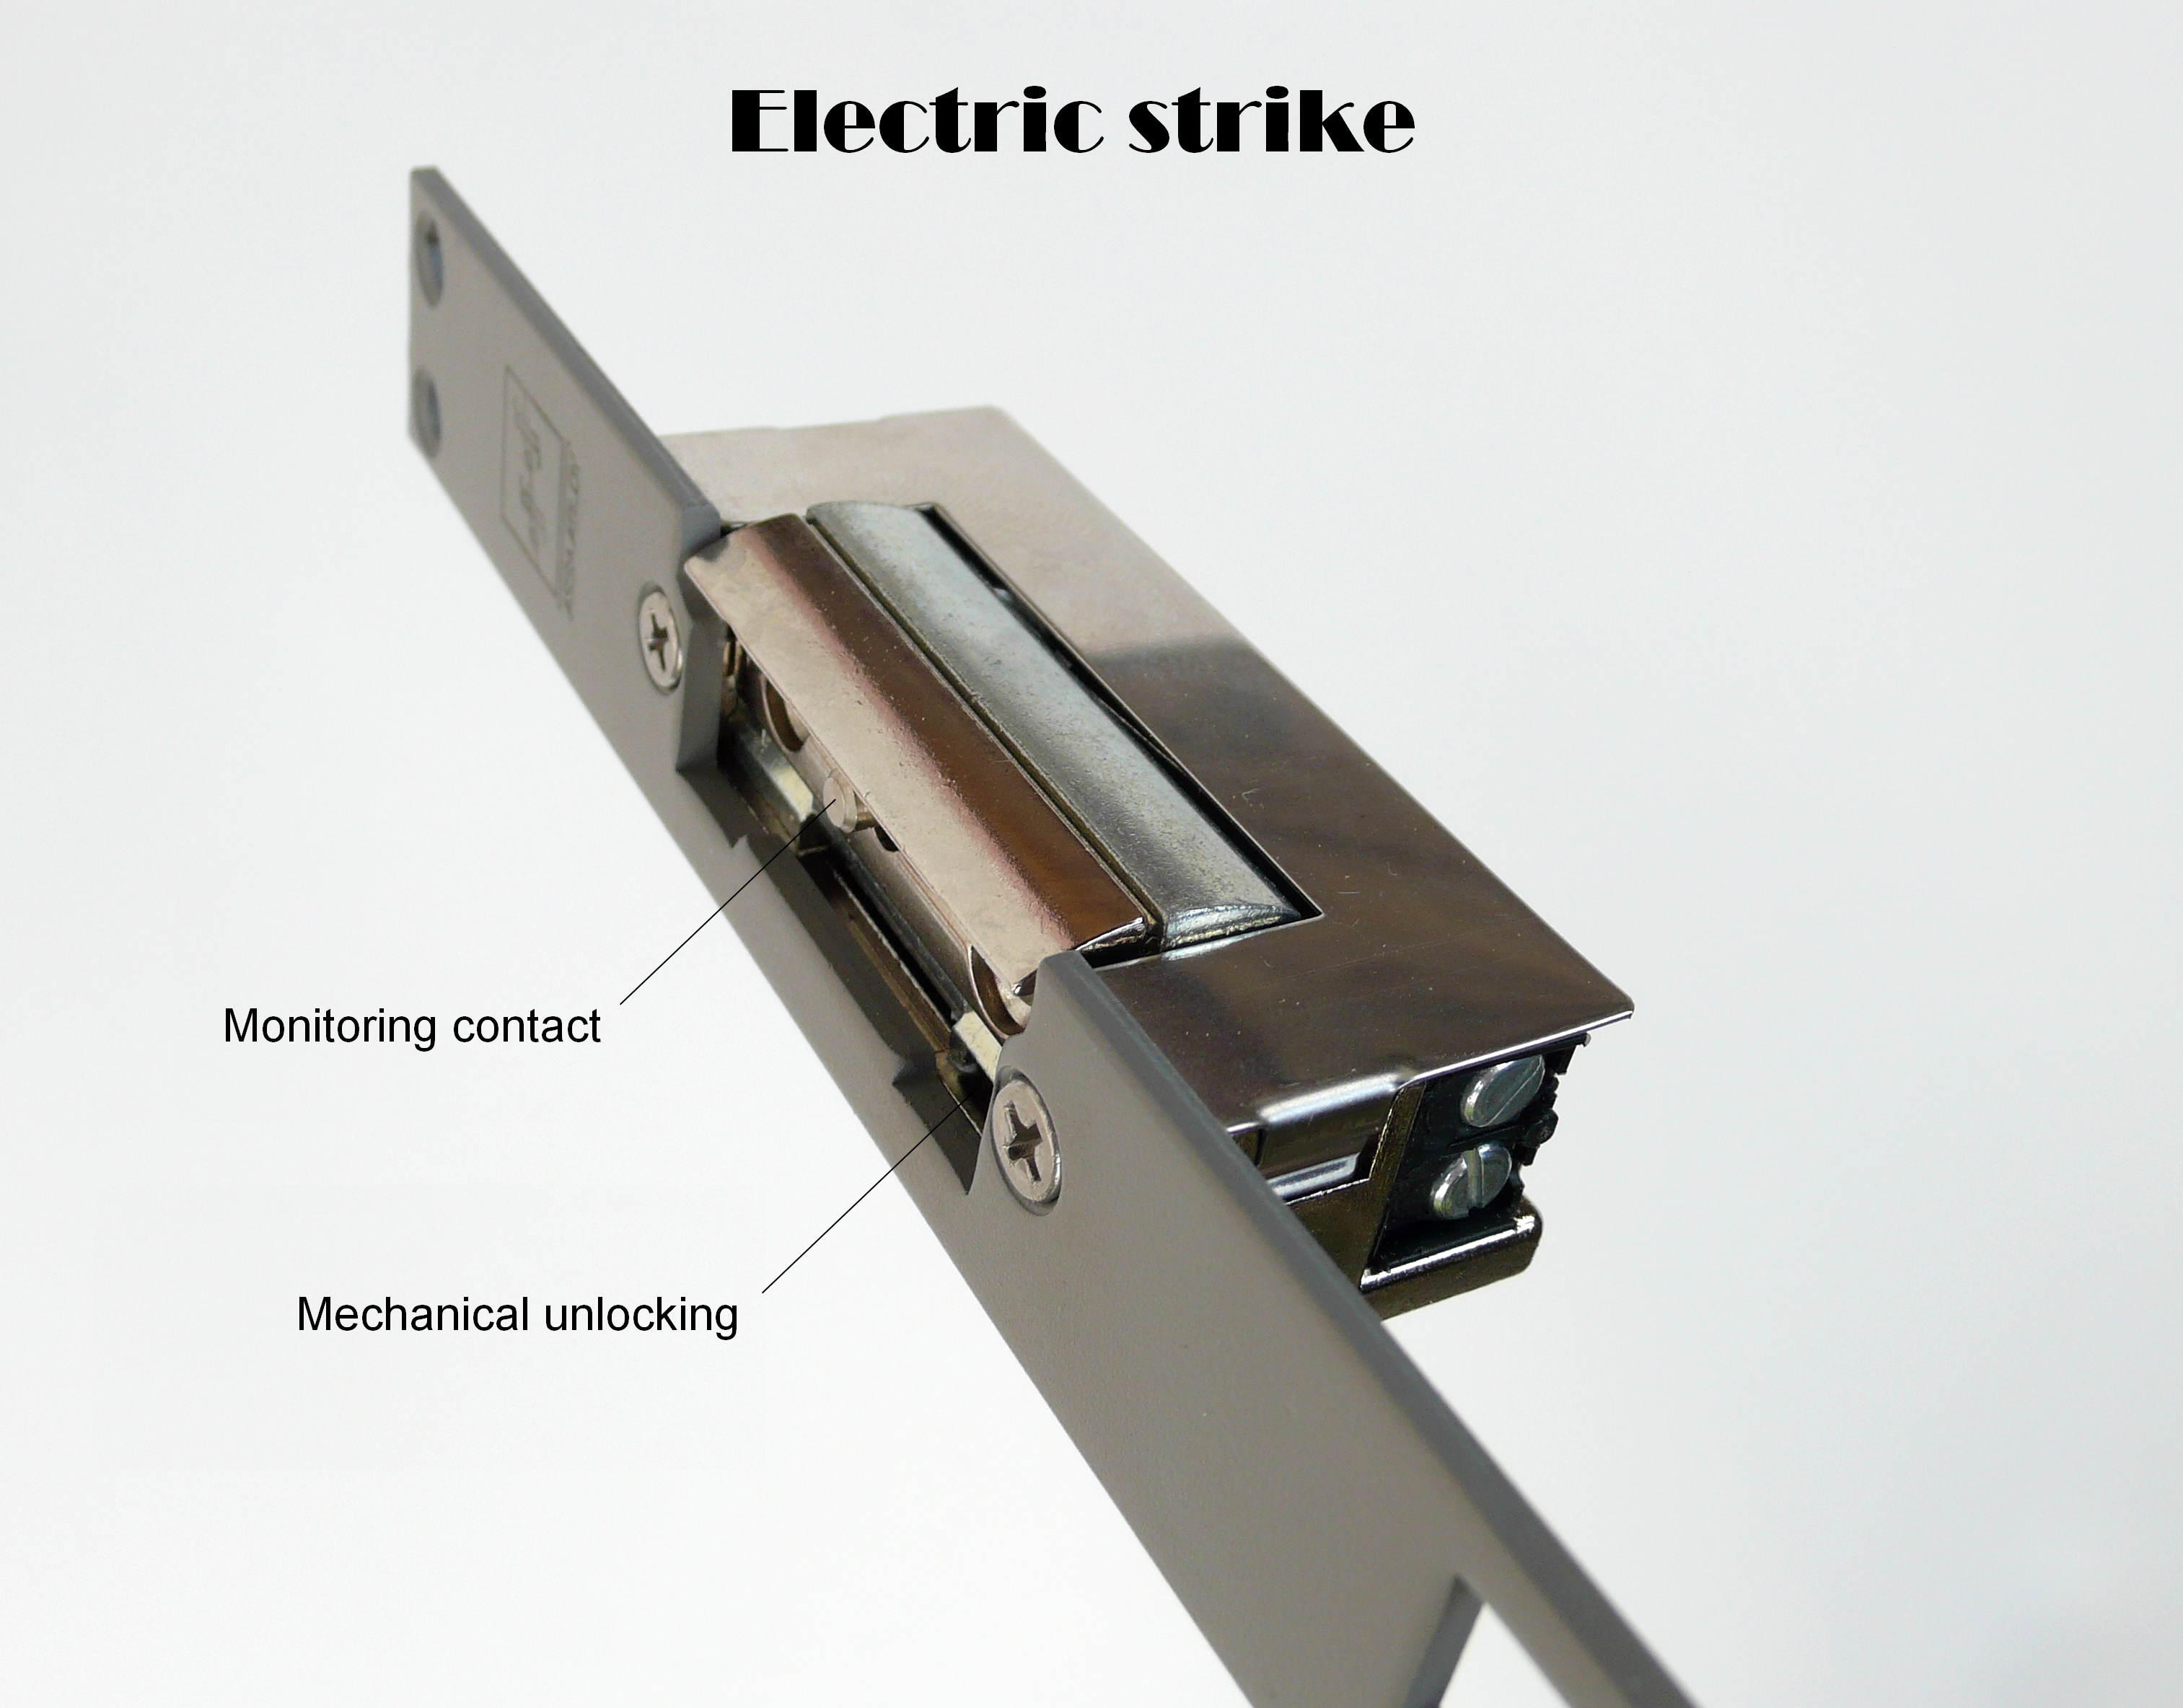
\includegraphics[width=0.5\textwidth,height=0.5\textheight,keepaspectratio]{Electric_strike.jpg}
	\caption{Ηλεκτρική κλειδαριά πολυκατοικίας με σύστημα καταγραφής κατάστασης κλειδώματος}
\end{figure}

Η ενεργοποίηση του παραπάνω συστήματος γίνεται μέσω ενός διακόπτη αναρτημένου πάνω στο θυροτηλέφωνο του κάθε διαμερίσματος. Η τροφοδοσία των συστημάτων αυτών μπορεί να γίνεται είτε μέσω απευθείας τροφοδοσίας από το ηλεκτρικό δίκτυο, είτε μέσω κάποιου μετασχηματιστή σε χαμηλότερες τάσεις.

Προκεικένου να μπορέσουμε να ελέγξουμε το σύστημα ξεκλειδώματος, θα πρέπει να μπορέσουμε να βάλουμε έναν δεύτερο διακόπτη, να λειτουργεί παράλληλα με τον πρώτο.  %TODO Refer to next chapter.

Για να γίνει αυτό, θα πρέπει να εντοπιστεί το κύκλωμα που συνδέεται με τον ήδη υπάρχοντα διακόπτη ξεκλειδώματος (του θυροτηλεφώνου) και να τοποθετηθούν 2 καλώδια σε παράλληλη σύνδεση με τον ήδη υπάρχοντα διακόπτη.

Για τον εντοπισμό θα πρέπει να αποσυνδεθεί ο διακόπτης από τον τοίχο, λύνοντας τις βίδες οι οποίες τον συγκρατούν. Προκειμένου να γίνει υπο ασφαλές συνθήκες, συνίσταται να απενεργοποιηθεί η παροχή ρεύματος στο παρόν τμήμα της οικίας, μέχρι να ολοκληρωθεί η εγκατάσταση. Αυτό μπορεί να γίνει είτε κατεβάζοντας την ασφάλεια που αντοιστοιχεί στο συγκεκριμένο τμήμα της κατοικίας, από τον ηλεκτρικό πίνακα, είτε απενεργοποιόντας τον γενικό διακόπτη τροφοδοσίας της κατοικίας.

Η τελική εγκατάσταση θα υπογραμμιστεί σε επόμενο κεφάλαιο.

    \chapter{Νέος μηχανισμός ξεκλειδώματος}
    Στο προηγούμενο κεφάλαιο είδαμε από τι αποτελείται ένα σύνηθες σύστημα ξεκλειδώματος πόρτας πολυκατοικίας/σπιτιού. Στο παρόν κεφάλαιο θα αναλύσουμε τον τρόπο σύνδεσης των εξαρτημάτων (βλ \fullref{sec:hardw}), και τον προγραμματισμό τους ώστε να μπορεί να πυροδοτηθεί ξεκλείδωμα της πόρτας μέσω υπολογιστή.

\section{Προετοιμασία του Raspberry Pi}
	Πρώτο βήμα πριν να γίνει η οποιαδήποτε σύνδεση μεταξύ εξαρτημάτων είναι αναγκαίο να γίνει η εγκατάσταση της τελευταίας έκδοσης του Raspbian Lite στο Raspberry Pi Zero W, καθώς επίσης και να συνδεθεί με το internet. Χρησιμοποιείται η έκδοση Lite έναντι της πλήρης έκδοσης, καθώς δεν χρειάζεται γραφικό περιβάλλον όπως επίσης και τα περισσότερα πακέτα που υπάρχουν προεγκατεστημένα στην πλήρη έκδοση.

	Αφότου γίνει η εγκατάσταση του λειτουργικού συστήματος στην κάρτα MicroSD, μπορεί να γίνει η σύνδεση στο Internet είτε Headlessly (χωρίς, δηλαδή, να χρειαστεί να συνδεθεί οθόνη στο RPi), βάζοντας το αρχείο στο \verb|boot| partition (διαμέρισμα) της κάρτας μνήμης, και εφαρμόζοντας το παρακάτω configuration, μέσα στο αρχείο \verb|wpa_supplicant.conf|\textsuperscript{\cite{rpi_wifi_headless}}:

	\begin{lstlisting}
	network={
		ssid="YOUR_NETWORK_NAME"
		psk="YOUR_PASSWORD"
	}\end{lstlisting} 

	Στο πεδίο \verb|ssid| πρέπει να μπει το όνομα του δικτύου στο οποίο πρόκειται να συνδεθεί το RPi. Στο πεδίο PSK πρέπει να γίνει τοποθέτηση του κλειδιού πρόσβασης του δικτύου. Σε περίπτωση που δεν χρησιμοποιείται κρυπτογραφία στο δίκτυο (δεν προτείνεται καθώς μπορεί να συμβεί υποκλοπή δεδομένων από τρίτους), μπορούμε να εισάγουμε το παρακάτω configuration στο ίδιο αρχείο:

	\begin{lstlisting}
	network={
		ssid="YOUR_NETWORK_NAME"
		key_mgmt=NONE
	}\end{lstlisting} 

	Τέλος, πρέπει να γίνει ενεργοποίηση του SSH Daemon στο Raspbian, προκειμένου να είναι εφικτή η απομακρυσμένη σύνδεση στο RPi, μέσω τοπικού δικτύου. Λόγω κατασκευής δικτύων bot (botnets) από διάφορους κακόβουλους χρήστες προκειμένου να γίνουν επιθέσεις DDOS (Distributed Denial of Service) από συσκευές Internet of Things που χρησιμοποιούν τα προεπιλεγμένα (default) στοιχεία πρόσβασης (Username, Password), προς διάφορους στόχους, από τον Νοέμβριο του 2016 είναι απενεργοποιημένος εξ' αρχής ο SSH Daemon και πρέπει να ενεργοποιηθεί από τον χρήστη, αν τον χρειάζεται \textsuperscript{\cite{raspbian_nov2016_upd}}. Για να γίνει αυτό, πρέπει να δημιουργηθεί ένα άδειο αρχείο με το όνομα \verb|ssh| μέσα στο \verb|boot| partition της κάρτας μνήμης του RPi.

	Αφότου γίνει η πρώτη εκκίνηση του RPi και βεβαιωθεί οτι υπάρχει ενεργή σύνδεση στο διαδίκτυο, πρέπει να γίνει σύνδεση στο Raspberry Pi μέσω SSH (Username: pi, Password: raspberry)\textsuperscript{\cite{default_creds}} και να γίνουν τα ακόλουθα βήματα, προκειμένου να ενημερωθεί πλήρως το Raspbian:

	\subsection{Αλλαγή των προεπιλεγμένων στοιχείων πρόσβασης}
		Όπως αναφέραμε προηγουμένως, προκειμένου να μην υπάρξει στο μέλλον κίνδυνος επίθεσης, πρέπει να γίνει αλλαγή των προεπιλεγμένων στοιχείων πρόσβασης στο Raspbian. Πρέπει να εκτελεστεί η εντολή \verb|passwd|, και να γίνει εισαγωγή ενός νέου κωδικού πρόσβασης. Ο νέος κωδικός, προκειμένου να είναι ασφαλής, πρέπει να αποτελείται από τουλάχιστον 12 χαρακτήρες, να μην περιέχει μέσα ονόματα, ονόματα από μέρη, ή γενικά λέξεις οι οποίες υπάρχουν μέσα σε λεξικά, και τέλος θα πρέπει να περιέχει πεζά γράμματα, κεφαλαία, αριθμούς, και σύμβολα\textsuperscript{\cite{secure_passwords}}.

	\subsection{Ενημέρωση του Raspbian}
		Προκειμένου να εξασφαλιστεί η βέλτιστη λειτουργία και η μέγιστη ασφάλεια στο σύστημα, χρειάζεται να γίνει ενημέρωση των πακέτων του λειτουργικού συστήματος. Πρέπει να γίνει εκτέλεση των επόμενων 2 εντολών\textsuperscript{\cite{raspbian_update}}:

		\begin{lstlisting}[language=bash]
		sudo apt-get update
		sudo apt-get dist-upgrade\end{lstlisting}

	Αφότου γίνει η αλλαγή των προεπιλεγμένων στοιχείων πρόσβασης και η ενημέρωση του συστήματος, πρέπει να απενεργοποιηθεί το σύστημα προκειμένου να συνδεθεί με το Relay. 

\section{Σύνδεση με το Relay}
	Για να γίνει η σύνδεση του Raspberry Pi με το Relay, πρέπει να επιλέξουμε έναν από τους 2 τρόπους σύνδεσης, ανάλογα με το τι Relay Module θα χρησιμοποιηθεί (βλ. \fullref{sub:relay}).

	\subsection{Σύνδεση χωρίς την χρήση Arduino}
		Προκειμένου να γίνει σύνδεση του RPi με το Relay Module, θα χρειαστεί να κολληθούν κεφαλές υποδοχής για Jumper Wires στα GPIO του Raspberry Pi. Μπορούν να χρησιμοποιηθούν είτε Female, είτε Male τύπου Headers, αλλά από αυτό θα εξαρτηθεί τι Jumper Wires θα χρειαστούν για να συνδεθεί το RPi με το Relay Module (Male-Female αν χρησιμοποιηθεί Female Header, Female-Female αν χρησιμοποιηθεί Male Header).

		\begin{figure}[h]
			\centering
				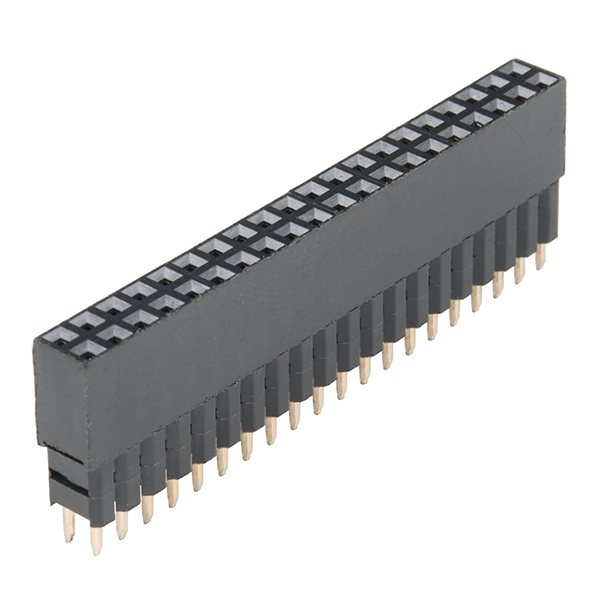
\includegraphics[width=0.5\textwidth,height=0.5\textheight,keepaspectratio]{female_gpio_headers.jpg}
			\caption{Female GPIO Headers, SparkFun Electronics (2016), Flickr, CC-BY 2.0}
			\label{fig:headers}
		\end{figure}

		Αφότου γίνει η κόλληση των Headers, μπορούν να χρησιμοποιηθούν τα αντίστοιχα καλώδια προκειμένου να συνδεθεί το Relay Module. Πρέπει ο χρήστης που θα το συνδέσει να συμβουλευτεί το διάγραμμα των GPIO Pins (γνωστό ως Pinout). Στο συγκεκριμένο παράδειγμα (\imgref{fig:rpi_to_relay}), έχει συνδεθεί στο GPIO Pin 18 (πράσινο καλώδιο). Για παροχή ρεύματος χρησιμοποιείται το 3V3 Pin (κόκκινο καλώδιο) και για Ground χρησιμοποιείται ένα από όλα τα GND Pins (μαύρο καλώδιο).

		\begin{figure}[h]
			\centering
				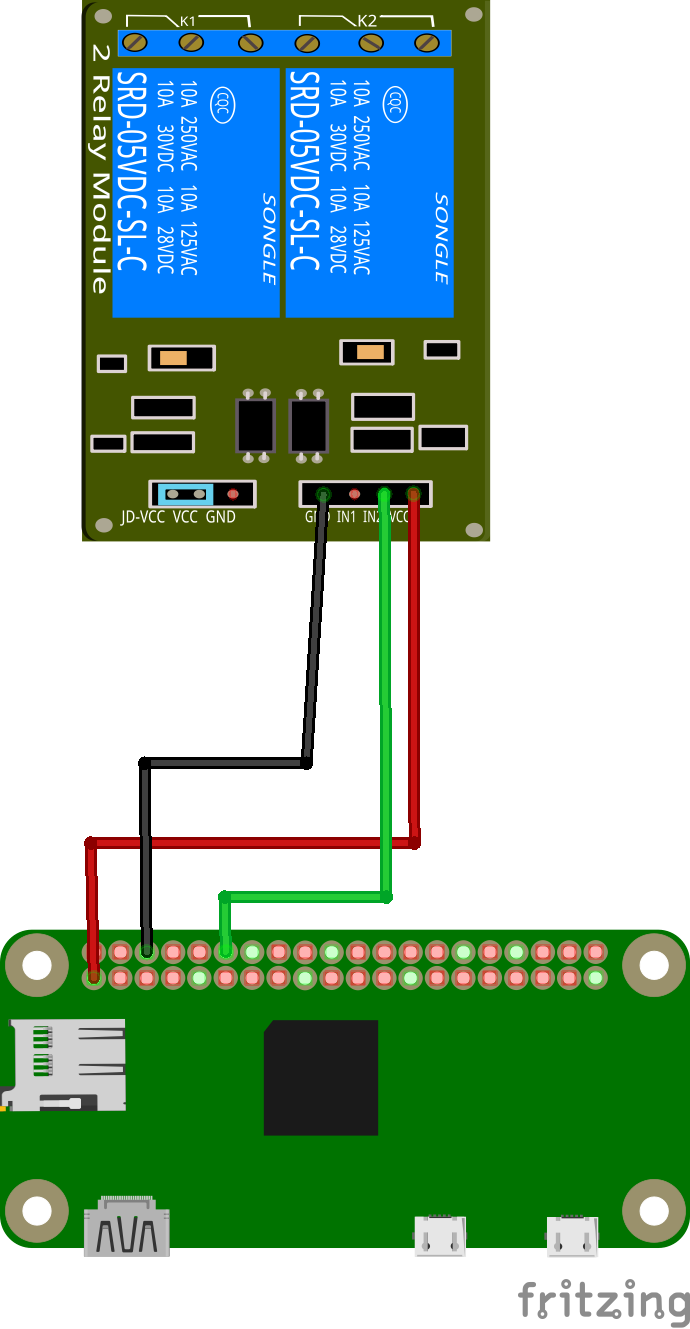
\includegraphics[width=0.5\textwidth,height=0.5\textheight,keepaspectratio]{rpi_to_relay.png}
			\caption{Σύνδεση ενός Raspberry Pi Zero W με ένα Relay Module}
			\label{fig:rpi_to_relay}
		\end{figure}


	\subsection{Σύνδεση με την χρήση Arduino}
		Αφότου γίνει Upload το Arduino Script που χρειάζεται για την λειτουργία του PiLock (βλ \fullref{sec:arduino_script}), μπορεί να γίνει σύνδεση του Arduino με το Relay. Το Relay Board μπορεί να συνδεθεί σε ένα από όλα τα Digital Pins του Arduino (πράσινο καλώδιο). Ρεύμα δίνεται μέσω του 5V Power Pin του Arduino και το Ground συνδέεται σε ένα εκ των τριών GND Pins του Arduino.

    \chapter{Προγραμματιστικό Περιβάλλον - Τεχνολογίες που Χρησιμοποιήθηκαν}
    Στο παρόν κεφάλαιο θα αναφερθούν και θα αναλυθούν τα εργαλεία που χρησιμοποιήθηκαν κατά την ανάπτυξη του PiLock, καθώς επίσης και στην διαχείρηση του έργου ανάπτυξης.

\section{Η σημασία χρήσης δωρεάν λογισμικού ανοικτού κώδικα κατά την ανάπτυξη του PiLock}
	Ως "Λογισμικό Ανοικτού Κώδικα" (Open Source Software) ορίζεται το λογισμικό του οποίου ο πηγαίος κώδικας είναι διαθέσιμος ελεύθερα προς το κοινό προκειμένου να μπορεί να τροποποιηθεί, να αναβαθμιστεί ή να μελετηθεί. Ο πηγαίος κώδικας, για τον απλό χρήστη είναι ένα τμήμα του λογισμικού που δεν έχει δει ποτέ. Σε έργα ανοικτού κώδικα, μπορεί ο οποιοσδήποτε να προτείνει διορθώσεις, αναβαθμίσεις ή προσθήκη χαρακτηριστικών\textsuperscript{\cite{FOSS_def}}. 

	Εξαιτίας αυτού του χαρακτηριστικού, και των αδειών που το υποστηρίζουν, το λογισμικό ανοικτού κώδικα μπορεί να χρησιμοποιηθεί για οποιοδήποτε σκοπό επιθυμεί ο χρήστης, χωρίς να περιορίζεται από κάποια άδεια χρήσης. Επίσης, παρέχει αυξημένη ασφάλεια, εφόσον μπορεί να δοκιμαστεί και να μελετηθεί από τους προγραμματιστές ο πηγαίος κώδικάς του. Στο λογισμικό κλειστού κώδικα, είναι αδύνατον να μελετηθεί και να τροποποιηθεί από τρίτους ο κώδικάς του, και κατ' επέκταση, εφόσον υπάρξει ένα κενό ασφαλείας θα πάρει συνήθως αρκετά περισσότερο χρόνο μέχρι να κυκλοφορήσει μια ενημέρωση ασφάλειας. Τέλος, εξαιτίας της ευελιξίας που παρέχει, το λογισμικό ανοικτού κώδικα μπορεί να τροποποιηθεί προκειμένου να μπορέσει καλύτερα να καλύψει τις ανάγκες του χρήστη\textsuperscript{\cite{FOSS_def}, \cite{FOSS_benefits}}.

	Μία υποκατηγορία του λογισμικού ανοικτού κώδικα είναι το \textbf{Δωρεάν Λογισμικό Ανοικτού Κώδικα (Free and Open Source Software, FOSS)}, το οποίο επιτρέπει στον χρήστη να το κατεβάσει και να το χρησιμοποιήσει χωρίς κάποιο κόστος. Το λογισμικό που χρησιμοποιήθηκε για την ανάπτυξη του PiLock ανήκει στην κατηγορία αυτή.

\section{Διαχείρηση του έργου}

	\subsection{Version Control}
		\label{subsec:vc}
		Καθ' όλη την διαδικασία ανάπτυξης του PiLock χρησιμοποιήθηκε σύστημα Version Control. Τα Συστήματα Version Control βοηθούν τον/τους προγραμματιστή/ές καθώς προσδίδουν ασφάλεια και ευελιξία κατά την ανάπτυξη και την συντήρηση ενός έργου. To \idxa{Git} είναι το λογισμικό Version Control που χρησιμοποιήθηκε κατά την ανάπτυξη του PiLock.

		Το Git δημιουργήθηκε από τον Linus Torvalds το 2005 προκειμένου να τον βοηθήσει στην ανάπτυξη του Linux Kernel\textsuperscript{\cite{Git_History}}. Διάφοροι άλλοι συνεισφέροντες προς το Linux Kernel βοήθησαν στην ανάπτυξη του Git, κατά την πρώτη περίοδο της ανάπτυξής του. Αποτελεί δωρεάν λογισμικό ανοικτού κώδικα και διανείμεται υπό την άδεια GNU General Public Licence, έκδοση 2\textsuperscript{\cite{Git_Licence}}. 

		Πιο συγκεκριμένα, εξαιτίας της ικανότητάς του Git να διατηρεί ιστορικό για όλα τα αρχεία ενός έργου, το έργο μπορεί να επανέλθει σε μία προηγούμενη κατάστασή του, ανά πάσα στιγμή. Οι "καταστάσεις" είναι γνωστές ως "\idxa{Commits}". Με αυτό τον τρόπο, δεν απορρίπτεται κώδικας, πολλές φορές πολύτιμος για την ανάπτυξη ενός έργου. Μέσω των commits, μπορεί κάποιος να βεβαιωθεί ποιος έκανε αλλαγές στον κώδικα σε οποιοδήποτε σημείο επιθυμεί. Αξίζει να αναφερθεί η δυνατότητα της ψηφιακής υπογραφής των commits μέσω του \idxa{GNU Privacy Guard (GPG)}, προκειμένου να αποφευχθεί προσωποποίηση\textsuperscript{\cite{Git_commit_assurance}}. Επίσης, μέσω του συστήματος \idxa{Staging} του Git, ο προγραμματιστής γνωρίζει τι ακριβώς κρατείται σε ένα νέο Commit, όποτε καταχωρηθεί. Με το \idxa{Branching System} του Git, καθίσταται δυνατόν να τροποποιείται ή να προστίθεται κώδικας και νέα features χωρίς να τροποποιείται ο Stable κώδικας του έργου (για παράδειγμα, το κάθε release χρησιμοποιεί υποχρεωτικά νέο branch), ο οποίος "ενημερώνεται" στο τέλος του κάθε release/feature, προκειμένου να αποφευχθούν προβλήματα. Τέλος, το Git διευκολύνει σημαντικά την συνεργασία μεταξύ προγραμματιστών καθώς μπορεί ο κάθε προγραμματιστής να δουλεύει το δικό του "κομμάτι" κώδικα, χωρίς να επηρρεάζει την πρόοδο των υπολοίπων προγραμματιστών που δουλεύουν πάνω στο έργο.

		Στην ανάπτυξη του PiLock, το λογισμικό της πλευράς του Εξυπηρετητή, του Πελάτη καθώς επίσης και τα σενάρια ξεκλειδώματος (Unlock Scripts) διαχειρίζονται ξεχωριστά σε διαφορετικά αποθετήρια. Συγκεκριμένα, τα σενάρια ξεκλειδώματος αποτελούν Submodule του λογισμικού του εξυπηρετητή, δηλαδή μπορεί να εμφολευθεί ως ξεχωριστό αποθετήριο μέσα σε ένα ήδη υπάρχον αποθετήριο, ως κομμάτι του.

		Προκειμένου να γίνει σωστή διαχείρηση της διαδικασίας ανάπτυξης, ακολουθήθηκαν κάποιοι κανόνες. Οι κανόνες αυτοί διασφαλίζουν την ακαιρεότητα του κώδικα ανα πάσα στιγμή κατά την ανάπτυξη. Πιο συγκεκριμένα:

		\begin{itemize}
			\item Η σταθερή (Stable) έκδοση του κώδικα βρίσκεται στο master branch.
			\item Όποια αλλαγή πρόκειται να γίνει στον κώδικα, είτε αυτή είναι hotfix, είτε κάποιο νέο feature, είτε documentation, θα πρέπει να γίνεται αποκλειστικά σε νέο branch με χαρακτηριστικό τίτλο, ο οποίος να ξεκινά από το ανάλογο πρόθεμα (prefix). Συγκεκριμένα, αν πρόκειται για νέο feature να χρησιμοποιείται το "feature" prefix, αν πρόκειται για bugfix να χρησιμοποιείται το "bug" ή το "hotfix" prefix, και αν πρόκειται για αλλαγή στο documentation ή στο Readme, να χρησιμοποιείται το "doc" prefix. (Πχ. feature/pin\_changing)
			\item Τα νέα Branches, εφόσον ελεγχθούν, θα πρέπει να συγχωνεύονται στο αντίστοιχο branch στο οποίο απευθύνονται (βλ. παρακάτω).
			\item Νέα λειτουργικότητα (νέα features) προστίθεται μόνο στα νέα releases (στο branch του εκάστοτε νέου release). Τα hotfix καθώς επίσης και διάφορα bugs μπορούν να συγχωνεύονται απευθείας με το master, αρκεί να έχουν ελεγχθεί εξονυχιστικά πρώτα και να είναι υψηλής προτεραιότητας.
			\item Το master branch, καθώς επίσης και τα branches για νέα releases θα πρέπει να είναι κλειδωμένα και να δέχονται συγχονεύσεις μόνο εφόσον περάσει από έγκριση ο κώδικας μέσω κάποιου \idxa{Pull Request} ή \idxa{Merge Request}.
		\end{itemize} 

		Αρχικά, μέχρι την πρώτη δημόσια έκδοσή του (\verb|0.2.0|), ο κώδικας του PiLock φιλοξενούνταν στον προσωπικό εξυπηρετητή του δημιουργού, και τα αποθετήρια του διαχειρίζονταν μέσω του δωρεάν λογισμικού διαχείρησης αποθετηρίων Git γνωστό ως \idxa{GitLab} (\url{https://about.gitlab.com}). Αργότερα, από την πρώτη δημόσια έκδοσή του PiLock και μετά, ξεκίνησε να χρησιμοποιείται το \idxa{GitHub} (\url{https://github.com}) ως χώρος φιλοξενίας του έργου και των αποθετηρίων του.

	\subsection{Issue Tracking}
		Κατά την ανάπτυξη του PiLock, έγινε χρήση τόσο του συστήματος Issue Tracking του GitLab, όσο και του GitHub. Τα συστήματα \idxa{Issue Tracking}, χρησιμοποιούνται για να κρατάνε μια λίστα με διάφορα "ζητήματα" που προκύπτουν κατά την ανάπτυξη ενός έργου ή που προέρχονται από εξωτερικούς χρήστες. Στην 2η κατηγορία ανήκουν διάφορα αιτήματα νέας λειτουργικότητας, ή διάφορα bugs τα οποία μπορεί να έχουν αναφερθεί, κατά την χρήση του λογισμικού ή κατά την διάρκεια δοκιμών (testing). Issues επίσης μπορεί να προκύψουν από εξωτερικούς χρήστες ως απλά ερωτήματα για την χρήση του λογισμικού.

		Τα Issues, έχουν 2 κύριες καταστάσεις: Open (Ανοικτό), Closed (Κλειστό/Ολοκληρωμένο). Τα ανοικτά issues είναι τα αυτά που ακόμα δεν έχουν ικανοποιηθεί οι απαιτήσεις τους, ή είναι σε διαδικασία ανάπτυξης. Τα κλειστά issues είναι τα εκπληρωμένα issues ή όσα issues δεν είναι δυνατόν να εκπληρωθούν για κάποιο λόγο, και δεν πρόκειται να αναπτυχθούν άλλο.

		Προκειμένου να μπορούν να κατηγοριοποιηθούν τα Issues ενός έργου, και να τα αναλάβουν, πολλές φορές διαφορετικές ομάδες, χρησιμοποιούνται οι ετικέτες (Labels). Κάποια χαρακτηριστικά παραδείγματα χρήσης ετικετών είναι για να χωριστούν τα issues που απαιτούν νέα λειτουργικότητα από τα issues που χρησιμοποιούνται προκειμένου να επιδιορθωθεί ένα bug.

		Όπως αναφέραμε στην αρχή, κατά την ανάπτυξη του PiLock, χρησιμοποιήθηκε Issue Tracking προκειμένου να οργανωθεί περισσότερο η διαδικασία της ανάπτυξης. Αξίζει να τονιστεί οτι έπειτα από την πρώτη δημόσια έκδοση του PiLock, μπορεί ο οποιοσδήποτε χρήστης του να συνεισφέρει στην συνεισφορά νέας λειτουργικότητας ή στην αναφορά και επίλυση bugs που υπάρχουν στο σύστημα.

		Το κάθε issue καταχωρείται στο αντίστοιχο milestone. Ως "\idxa{Milestone}" (Ορόσημο) ορίζεται ένα σημαντικό σημείο κατά την ανάπτυξη του έργου. Τα Milestones δημιουργούνται από τους συντηρητές ή τους διαχειριστές ενός έργου και χρησιμοποιούνται προκειμένου να οργανωθεί καλύτερα η ανάπτυξη του έργου και για να κατηγοριοποιηθούν τα issues. Για παράδειγμα, ως milestones συνήθως ορίζονται οι νέες εκδόσεις ενός έργου, πριν να γίνουν stable. Αφότου γίνουν Stable, το milestone κλείνει.

\section{Προγραμματιστικό Περιβάλλον}
	\label{sec:ides}
	\subsection{Γλώσσες Προγραμματισμού/Markup}
		Το λογισμικό που χειρίζεται το \idxa{Business Logic} του εξυπηρετητή του PiLock ήταν, αρχικά, γραμμένο σε Python 2.7. Από την έκδοση \verb|0.3.1| και έπειτα, έγινε μετάβαση στην Python 3.6. Το γραφικό περιβάλλον είναι γραμμένο σε \idxa{HTML5 (HyperText Markup Language)}, \idxa{CSS3 (Cascading Style Sheets)} και \idxa{JavaScript}. Το αρχείο παραμετροποίησης που χρησιμοποιείται μέχρι και την τελευταία έκδοση, προκειμένου να μπορεί ο χρήστης, αν θέλει, να κλειδώσει το PiLock, είναι γραμμένο σε \idxa{YAML} (YAML Ain't Another Markup Language). Τέλος, τα σενάρια που χρησιμοποιούνται για την αρχική εγκατάσταση του PiLock στο RPi, είναι γραμμένα σε \idxa{Shell}. Το λογισμικό της εφαρμογής Android, καθώς επίσης και της εφαρμογής για Android Wear, είναι γραμμένα σε Java και \idxa{XML (Cross Markup Language)}. Τα σενάρια ξεκλειδώματος (Unlock Scripts) είναι γραμμένα σε Python και \idxa{Wiring}, ένα Framework κατασκευασμένο για προγραμματισμό μικροελεγκτών, το οποίο χρησιμοποιείται για προγραμματισμό στο Arduino.

	\subsection{Βιβλιοθήκες/Frameworks που χρησιμοποιήθηκαν}
		\label{sub:fws}
		Το Business Logic του εξυπηρετητή του PiLock είναι υλοποιημένο σε Django. Το Django είναι ένα Free And Open Source Web Framework γραμμένο σε Python και συντηρείται από το Django Software Foundation (DSF)\sucite{DSF}. Χρησιμοποιεί την αρχιτεκτονική MVT (Model-View-Template). Το Django είναι φτιαγμένο προκειμένου να καταστήσει εύκολη την ανάπτυξη πολύπλοκων ιστοσελίδων, που χρησιμοποιούν σύνδεση με βάσεις δεδομένων. Βασίζεται στην αρχή του Don't Repeat Yourself (DRY), που σημαίνει οτι είναι έτσι σχεδιασμένο, ώστε να μπορέσει να μειώσει τις επαναλήψεις κομματιών κώδικα, η την επανάληψη ορισμού λειτουργικότητας σε ένα λογισμικό\sucite{Django_Philosophies}. Το Django παρέχει σύστημα αφαιρετικότητας βάσεων δεδομένων (Database Abstraction), που σημαίνει οτι ο τελικός κώδικας είναι συμβατός με μια πληθώρα συστημάτων βάσεων δεδομένων (sqlite, MySQL, PostgreSQL). Αυτό καθιστά την μετάβαση του συστήματος (αν χρειαστεί), σε κάποιο νέο σύστημα βάσης δεδομένων εύκολη, καθώς δεν χρειάζεται να αλλάξει ο κώδικας.

		Ο πίνακας διαχείρησης του PiLock (AdminCP), χρησιμοποιεί το Bootstrap 3 framework προκειμένου να εξασφαλίσει ομαλή έμφάνιση των οπτικών στοιχείων του σε όλα τα πιθανά μεγάθη οθονών. Το Bootstrap δημιουργήθηκε από τον Mark Otto και τον Jacob Thornton, που εργάζονταν ως προγραμματιστής και designer, αντίστοιχα, στο Twitter το 2010 \textsuperscript{\cite{BS_about}}, όπου προέκυψε ανάγκη για ενοποίηση των εργαλείων που χρησιμοποιούνταν προκειμένου να είναι λιγότερο δαπανηρή η συντήρηση\sucite{BS_cr_reason}. Το Twitter είναι ένα Free and Open Source έργο, και διανείμεται υπό την άδεια MIT.
 		
 		Προκειμένου να μπορούν να εκτελεστούν κάποιες λειτουργίες του πίνακα διαχείρησης, όπως το ξεκλείδωμα απευθείας από τον πίνακα διαχείρησης, καθώς επίσης και κάποια οπτικά εφέ, χρησιμοποιήθηκε η βιβλίοθήκη jQuery. H jQuery είναι μια βιβλιοθήκη γραμμένη σε Javascript και χρησιμοποιείται προκειμένου να απλοποιήσει την διαδικασία προγραμματισμού στο επίπεδο του πελάτη (Client-Side Scripting)\sucite{JQ_about}.

 	\subsection{Προγραμματιστικά Εργαλεία που Χρησιμοποιήθηκαν}
 		Καθ' όλη την διαδικασία ανάπτυξης του PiLock, χρησιμοποιήθηκαν διάφορα \textbf{Ολοκληρωμένα Περιβάλλοντα Ανάπτυξης (Integrated Development Environments, IDE)}, τα οποία, κάποια εξ' αυτών αποτελούν λογισμικό ανοικτού κώδικα. Παρατίθενται παρακάτω.

 		\subsubsection{PyCharm - JetBrains}
 			Το PyCharm είναι ένα προγραμματιστικό περιβάλλον στοχευμένο στην ανάπτυξη λογισμικού με την γλώσσα Python. Αναπτύσσεται από την τσεχική εταιρία JetBrains\sucite{Pycharm_creator} και είναι γραμμένο σε Java και Python. Διατίθενται 2 εκδόσεις του Pycharm: Το PyCharm Community, που είναι δωρεάν και ανοικτού κώδικα λογισμικό (υπόκειται, συγκεκριμένα, στην άδεια Apache\sucite{Pycharm_comm_FOSS}), και το PyCharm Professional, το οποίο διατίθεται επι πληρωμής και είναι κλειστού κώδικα. Το PyCharm Professional παρέχει επιπρόσθετη λειτουργικότητα από αυτή του Community. Και οι δύο εκδόσεις είναι συμβατές με Windows, Linux και macOS.

 			Το PyCharm περιέχει λειτουργικότητα ανάλυσης κώδικα, γραφικό αποσφαλματωτή (graphical debugger), και ενσωμάτωση πολλών εργαλείων διαχείρησης εκδόσεων (βλ. \fullref{subsec:vc}), προκειμένου να ελαττωθεί η χρήση αυτών των προγραμμάτων εκτός του περιβάλλοντος εργασίας.

 			Το PyCharm επιλέχτηκε κατά την ανάπτυξη του PiLock Server κυρίως λόγω του γραφικού αποσφαλματωτή, της ανάλυσης κώδικα και της ενσωμάτωσης εργαλείων διαχέιρησης εκδόσεων. Από την έκδοση \verb|0.3.1| και έπειτα, χρησιμοποιήθηκε επίσης η λειτουργία Unit Testing που παρέχει προκειμένου να υλοποιηθεί μηχανισμός αυτοματοποιημένου ελέγχου εγκυρότητας κώδικα (βλ. \fullref{sec:unittesting}).

 		\subsubsection{Android Studio}
 			Για την ανάπτυξη της εφαρμογής Android και αργότερα, από την έκδοση \verb|0.3.0| και μετά, για την ανάπτυξη της εφαρμογής για Android Wear, χρησιμοποιήθηκε το Android Studio. Το \idxa{Android Studio} αποτελεί το επίσημο περιβάλλον ανάπτυξης εφαρμογών για Android συστήματα. Κατασκευάζεται από την Google σε συνεργασία με την JetBrains και είναι βασισμένο πάνω στο IntelliJ IDEA της JetBrains. Είναι γραμμένο σε Java και Kotlin.

 			Το Android Studio αποτελεί αντικαταστάτη των Εργαλείων Ανάπτυξης Android του Eclipse (Android Development Tools, ADT), τα οποία χρησιμοποιούνταν για ανάπτυξη σε Android μέχρι και το 2015\sucite{adt_deprecation}.

 		\subsubsection{Άλλα Εργαλεία, Text Editors}
 			\paragraph{Sublime Text}
 				Το \idxa{Sublime Text} είναι ένας επεξεργαστής κειμένου γραμμένος σε C++ και Python από τον Jon Skimmer και τον Will Bond. Υποστηρίζει μια πληθώρα γλωσσών προγραμματισμού και με λειτουργικότητα όπως η "Goto Anything", η οποία υποστηρίζει γρήγορη πλοήγηση σε οποιοδήποτε σημείο του κώδικα, σε διάφορα αρχεία, σύμβολα ή γραμμές επιλέγεται από πολλούς προγραμματιστές ανά τον πλανήτη.

 				Στο PiLock χρησιμοποιήθηκε κατά την ανάπτυξη μέρους του γραφικού περιβάλλοντος του πίνακα διαχείρησης συγκεκριμένα για την δημιουργία και επεξεργασία των αρχείων HTML5, CSS3 και JavaScript που τον αποτελούν.

 			\paragraph{GNU Nano}
 				Ο \idxa{GNU Nano} είναι ένας επεξεργαστής κειμένου που χρησιμοποιεί γραφική διεπαφή γραμμής εντολών (Command Line Graphical User Interface) και υπάρχει προεγκατεστημένος στα περισσότερα συστήματα είδους Unix. Είναι φτιαγμένος έτσι ώστε να μπορεί να εξομοιώνει τον Pico Editor όσο το δυνατόν καλύτερα και παράλληλα παρέχει παραπάνω λειτουργικότητα από αυτόν\sucite{nano_extra}. Είναι δωρεάν και ανοικτού κώδικα λογισμικό και υπόκειται στην άδεια GNU General Public Licence (GPL).

 				Κατά την ανάπτυξη του PiLock, το GNU Nano χρησιμοποιήθηκε προκειμένου να γίνουν δοκιμές και αποσφαλμάτωση του PiLock Server, ενόσω είναι σε λειτουργία πάνω στο Raspberry Pi, καθώς είναι προσβάσιμο από απομακρυσμένο τερματικό, μέσω SSH.

 			\paragraph{git-cola}
 				Το \idxa{git-cola} είναι ένα δωρεάν και ανοικτού κώδικα γραφικό περιβάλλον διαχείρησης αποθετηρίων Git, ανεπτυγμένο από τον David Aguilar σε Python, και χρησιμοποιεί την βιβλιοθήκη PyQt για την κατασκευή του γραφικού περιβάλλοντός του. Χρησιμοποιείται προκειμένου να καταστεί πιο εύκολη η διαχείρηση ενός αποθετηρίου git, παρέχοντας μεγάλο μέρος των λειτουργιών του git μέσω του εύχρηστου γραφικού περιβάλλοντός του. Υποστηρίζει λειτουργίες όπως ευανάγνωστη προβολή του ιστορικού του αποθετηρίου, εύχρηστη λειτουργία δημιουργίας νέων commits, και πολλές άλλες. Yπόκειται στην άδεια GNU General Public Licence (GPL), version 2\sucite{gitcola_licence}.

    \chapter{Χρονοδιάγραμμα Κυκλοφορίας Εκδόσεων}
    Το PiLock κυκλοφορεί σε συγκεκριμένες εκδόσεις. Η κάθε έκδοση μπορεί να παρέχει είτε αυξημένη λειτουργικότητα, είτε αλλαγές προκειμένου να βελτιστοποιηθεί ο ήδη υπάρχον κώδικας. Υπάρχουν 2 τύπου εκδόσεις, Minor (μικρές), Major (μεγάλες). Οι μικρές εκδόσεις συνεισφέρουν μικρές αλλαγές στην λειτουργικότητα του PiLock, και συνήθως αποτελούνται αποκλειστικά από βελτιστοποιήσεις στον κώδικα και διορθώσεις bugs. Οι μεγάλες εκδόσεις συνεισφέρουν μεγάλες αλλαγές στην λειτουργικότητα είτε του πελάτη, είτε του εξυπηρετητή και συνήθως περιέχουν πολλά bugfix.

Στις μεγάλες εκδόσεις γίνεται αλλαγή στο νούμερο ανάμεσα στην 1η και την 2η υποδιαστολή του κωδικού έκδοσης. Στις μικρές εκδόσεις αλλάζει το νούμερο μετά την 2η υποδιαστολή, από αριστερά. Συγκεκριμένα, με κάθε νέα ενημέρωση, γίνεται αύξηση κατά ένα του αντίστοιχου αριθμού. Αν είναι μεγάλη έκδοση, πρέπει να γίνει επαναφορά του αριθμού μικρής έκδοσης στο μηδέν (0).

Παρακάτω παρατίθενται οι εκδόσεις από την δημιουργία του PiLock, μέχρι τώρα. Έχουν επίσης αναρτηθεί συνοπτικά διαγράμματα των κλάσεων που χρησιμοποιήθηκαν, στο \apref{ap:version_class_diag}, καθώς επίσης και αναλυτικά διαγράμματα περιπτώσεων χρήσης (Use Case) στο \apref{ap:version_usecase_diag}.

\section{0.1.0}
	Ημερομηνίες ανάπτυξης:\\Έναρξη: 1η Απριλίου 2017\\Κυκλοφορία: 17 Μαϊου 2017

	Η έκδοση \verb|0.1.0| ήταν η 1η έκδοση που βγήκε από την πρώτη σύλληψη του PiLock και μετά και παρείχε την βασική λειτουργικότητα, αρκετή για να λειτουργήσει το κύκλωμα ξεκλειδώματος. 

	Μέχρι τότε, η εφαρμογή πελάτη για Android είχε πολλά προβλήματα κατά την λειτουργία της, με πολλά crash, αλλά το βασικό σύστημα ξεκλειδώματος είχε υλοποιηθεί και δούλευε.

\section{0.2.0}
	Ημερομηνίες ανάπτυξης:\\Έναρξη: 29 Ιουλίου 2017\\Κυκλοφορία: 18 Αυγούστου 2017

	Η έκδοση \verb|0.2.0| αποτελεί την πρώτη δημόσια διαθέσιμη έκδοση του PiLock. Σε αυτή την έκδοση έγινε η προσθήκη του πίνακα διαχείρησης στην πρωτογενή μορφή του (πριν την κυκλοφορία της έκδοσης αυτής, οι χρήστες έπρεπε να χρησιμοποιήσουν τον συμπεριλαμβανόμενο στο Django πίνακα διαχείρησης).

	Επίσης, έγινε μια τεράστια αλλαγή στον οπτικό σχεδιασμό της εφαρμογής. Το κύριο χρώμα της εφαρμογής mobile άλλαξε σε ρόζ (\verb|#790022|) και έγινε προσθήκη ενός νέου λογότυπου φτιαγμένο από τον Δημήτρη Τζιλιβάκη.

	Στον πίνακα διαχείρησης προστέθηκε δυνατότητα διαχείρησης χρηστών, συγκεκριμένα, λειτουργία προσθήκης νέων και διαγραφής ήδη υπάρχοντων χρηστών και προφίλ συσκευών, καθώς επίσης και ένα ημερολόγιο ξεκλειδωμάτων και συνδέσεων στο σύστημα, για λόγους ασφάλειας.  

\section{0.3.0}
	Ημερομηνίες ανάπτυξης:\\Έναρξη: 7 Σεπτεμβρίου 2017\\Κυκλοφορία: 11 Νοεμβρίου 2017

	Στην έκδοση \verb|0.3.0| προστέθηκε πλήθος νέων λειτουργιών που βοηθούν στην διαχείρηση και στην χρήση του PiLock. Προστέθηκε, συγκεκριμένα δυνατότητα ξεκλειδώματος χωρίς την χρήση PIN, ένα νέο σύστημα ειδοποιήσεων προσβάσιμο από τον πίνακα διαχείρησης από όπου ο χρήστης μπορεί να δει διάφορα μηνύματα σχετικά με την κατάσταση του PiLock, καθώς επίσης και δυνατότητα ξεκλειδώματος μέσω του πίνακα διαχείρησης.

	Στην νέα λειτουργικότητα εντάσσεται επίσης η εφαρμογή για Android Wear συσκευές, που επιτρέπει στον χρήστη, εφόσον είναι συνδεδεμένο το SmartPhone του με το Smartwatch του, να γίνει ξεκλείδωμα, μέσω του Android Wear Smartwatch του.

	Τέλος, προστέθηκε hashing στην βάση δεδομένων προκειμένου να αποτρέψει προβολή των κλειδιών πρόσβασης σε περίπτωση που υπάρξει μη εξουσιοδοτημένη πρόσβαση στην βάση δεδομένων\sucite{pw_hashing} (βλ \fullref{subsec:login_stage}). 


\section{0.3.1}
	Ημερομηνίες ανάπτυξης:\\Έναρξη: 25 Φεβρουαρίου 2018\\Κυκλοφορία: 4 Μαρτίου 2018

	Στην Minor έκδοση \verb|0.3.1| του PiLock, έγινε ενημέρωση του κώδικα ώστε να χρησιμοποιείται πλέον η Python 3.6, καθώς η Python 2.7 φτάνει σιγά σιγά στο τέλος ζωής της\sucite{Py27EOL} και οι νέες ενημερώσεις για το Django θα γίνονται μόνο στην έκδοση 3 της Python\sucite{Django_NewUpdates}. Έγιναν πολλές διορθώσεις στον κώδικα του Server, προκειμένου να λειτουργεί καλύτερα, ενεργοποιήθηκε η χρήση του venv και ενεργοποιήθηκε η δυνατότητα αυτοματοποιημένων ελέγχων εγκυρότητας κώδικα μέσω Continuous Integration (CI).

	Από άποψης λειτουργικότητας, έγινε προσθήκη σελιδοποίησης στο ημερολόγιο πρόσβασης του συστήματος, προκειμένου να φαίνονται οι απόπειρες πρόσβασης πιο καθαρά.


    \chapter{Σενάρια Ξεκλειδώματος - PiLockUnlockScripts}
    Τα σενάρια (scripts) ξεκλειδώματος του PiLock, γνωστά ως PiLockUnlockScripts, αποτελούν κομμάτι του λογισμικού του εξυπηρετητή. Συνδέονται με το Django Project του εξυπηρετητή μέσω ενός Git Submodule που έχει τοποθετηθεί στο main app.

Η δέσμη των σεναρίων αποτελείται από ένα σενάριο γραμμένο σε Python και ένα πρόγραμμα Arduino, σε περίπτωση που ο χρήστης επιθυμεί να χρησιμοποιήσει Arduino για να πραγματοποιεί ξεκλείδωμα (βλ. \fullref{subsec:arduino_conn}).

\begin{lstlisting}[language=python, caption=Σενάριο Ξεκλειδώματος Python (unlock.py), label={lst:python_unlockscript}]
	import serial
	from time import sleep
	import RPi.GPIO as GPIO

	# Mode switch
	# 0 -> GPIO Unlock
	# 1 -> Arduino Assisted Unlock (default before 0.3.1)
	MODE = 0
	# The GPIO pin used for the switch. Refer to your RPi's PinOut diagram.
	# Used only when MODE = 0 
	SW_PIN = 18 

	def unlock():
	    if MODE == 0:
	        GPIO.setmode(GPIO.BCM)
	        GPIO.setwarnings(False)
	        GPIO.setup(SW_PIN, GPIO.OUT)
	        GPIO.output(SW_PIN, GPIO.HIGH)
	        sleep(5)
	        GPIO.output(SW_PIN, GPIO.LOW)
	        GPIO.cleanup()
	    else:
	        ser = serial.Serial(port="/dev/ttyACM0", baudrate=9600)
	        ser.isOpen()
	        sleep(2)  # Wait for the arduino to be ready.
	        ser.write(b"ENABLE")
	        ser.close()

	if __name__ == "__main__":
	    unlock()\end{lstlisting}

\section{Ξεκλείδωμα μέσω GPIO}
	Ο προεπιλεγμένος τρόπος ξεκλειδώματος, από την έκδοση \verb|0.3.1| και έπειτα, είναι το ξεκλείδωμα μέσω των δεκτών GPIO του Raspberry Pi. Αφότου συνδεθεί το Raspberry Pi με ένα συμβατό Relay Module (βλ. \fullref{subsec:gpio_conn}), μπορεί να εκτελεστεί το προεπιλεγμένο σενάριο ξεκλειδώματος (\fullref{lst:python_unlockscript}).

	Προκειμένου να οριστεί ο τρόπος ξεκλειδώματος, πρέπει να αλλάξει η μεταβλητή \verb|MODE| σε 0, αν πρόκειται να χρησιμοποιηθεί το GPIO ως μέθοδος ξεκλειδώματος, και οτιδήποτε άλλο αν πρόκειται να χρησιμοποιηθεί Arduino για ξεκλείδωμα.

	Αν πρόκειται να χρησιμοποιηθεί το GPIO ως μέθοδος ξεκλειδώματος, πρέπει να γίνει επίσης τροποποίηση της μεταβλητής \verb|SW_PIN|, προκειμένου να οριστεί το GPIO Pin το οποίο θα χρησιμοποιηθεί για το Relay. Στο παράδειγμα \autoref{fig:rpi_to_relay}, χρησιμοποιείται το Pin \#18, κατά BCM\sucite{rpi_pinout}.

	Στην γραμμή 15, ορίζεται η λειτουργία αρίθμησης ως BCM και στην 16 γίνεται απενεργοποίηση των προειδοποιήσεων του συστήματος GPIO. Στην γραμμή 17 γίνεται ορισμός του GPIO Pin που ορίστηκε από την μεταβλητή \verb|SW_PIN| ως έξοδος. Στις γραμμές 18, 19 και 20 πραγματοποιείται το ξεκλείδωμα. Συγκεκριμένα, στέλνεται ψηφιακό σήμα 1 στο Relay Module μέσω του Pin εξόδου που έχει οριστεί. Κατά την συγκεκριμένη χρονική στιγμή, ο μηχανισμός ξεκλειδώματος της πόρτας (βλ. \fullref{ch:unlock_mechanism}) δέχεται ρεύμα και ενεργοποιείται, δηλαδή μπορεί κάποιος, αν σπρώξει την πόρτα, να την ανοίξει. Το σύστημα παραμένει στην συγκεκριμένη κατάσταση  για 5 δευτερόλεπτα (γραμμή 19) και έπειτα ξαναγυρνά το Pin εξόδου σε 0, και απενεργοποιείται ο μηχανισμός ξεκλειδώματος (γραμμή 20). Τέλος, γίνεται εκκαθάριση των GPIO (γραμμή 21). Το ξεκλείδωμα ολοκληρώθηκε.

\section{Ξεκλείδωμα μέσω Arduino}
	Προκειμένου να καταστεί δυνατόν να πραγματοποιούνται ξεκλειδώματα μέσω Arduino, θα πρέπει πρώτα να γίνει μεταφόρτωση του ακόλουθου σεναρίου προγραμματισμού στο Arduino, μέσω του Arduino IDE:

	\begin{lstlisting}[language=C++, caption=Σενάριο Ξεκλειδώματος Arduino, label={lst:arduino_unlockscript}]
	// The pin the relay is attached to.
	const int RELAY_PIN = 2;
	// How many seconds to keep the relay turned on.
	const int DELAY = 5;

	void setup() {
	  // Setup everything...
	  Serial.begin(9600);
	  pinMode(RELAY_PIN, OUTPUT);
	  pinMode(LED_BUILTIN, OUTPUT);
	}

	void loop() {
	  // The Relay is active low, so write high to it in order to disable it.
	  digitalWrite(RELAY_PIN, HIGH);
	  digitalWrite(LED_BUILTIN, LOW);

	  // If the serial port is available, read each character and concatenate it to a string.
	  if (Serial.available() > 0){
	    String content = "";
	    char character;

	    while(Serial.available()) {
	        character = Serial.read();
	        content.concat(character);
	        delay(10); // Add a 10ms delay in order to receive the characters correctly.
	    }

	    // Finally, check the string, if it reads "ENABLE", turn on the relay, wait for 5 seconds, then turn it off.
	    if (content == "ENABLE") {
	      digitalWrite(RELAY_PIN, LOW);
	      digitalWrite(LED_BUILTIN, HIGH);
	      delay(DELAY * 1000);
	    }
	  }
	}\end{lstlisting}

	Προκειμένου να γίνει αντιληπτό το παραπάνω σενάριο, είναι αναγκαίο να αναλυθεί η ανάγκη χρήσης της σειριακής θύρας του Arduino. Όλες οι πλακέτες Arduino έχουν τουλάχιστον μία Hardware-Based σειριακή θύρα. Αυτή χρησιμοποιείται προκειμένου να γίνει ανταλλαγή δεδομένων με κάποιο υπολογιστή ή με κάποια άλλη συσκευή συνδεδεμένη στο Arduino\sucite{arduino_serial}. Στο PiLock, η σειριακή θύρα του Arduino χρησιμοποιείται για να ενεργοποιήσει το Arduino το Relay Module, την στιγμή που είναι επιθυμητό. Συγκεκριμένα, όταν η σειριακή θύρα λάβει την λέξη "ENABLE", γίνεται ενεργοποίηση του Relay Module (γραμμές 30-34). Στις γραμμές 23-27 γίνεται σχηματισμός της λέξης με έναν χαρακτήρα την φορά, καθώς λαμβάνεται από την σειριακή θύρα.

	Και πάλι χρησιμοποιείται η ίδια λογική ενεργοποίησης του Relay Module με αυτή που χρησιμοποιείται όταν γίνεται ξεκλείδωμα μέσω GPIO, αλλά σε αυτή την περίπτωση γίνεται αντίστροφα (0 για ενεργοποίηση, 1 για απενεργοποίηση), καθώς το σενάριο είναι γραμμένο για Relays που δουλεύουν με λογική Active Low. Μπορεί να γίνει τροποποίηση του σεναρίου για να λειτουργεί με Active High Relay Modules, αλλάζοντας τις λέξεις \verb|HIGH| σε \verb|LOW| και αντίστροφα.

	Την αποστολή της λέξης στο Arduino αναλαμβάνει το σενάριο ξεκλειδώματος \verb|unlock.py| που αναφέρθηκε προηγουμένως (\fullref{lst:python_unlockscript}). Συγκεκριμένα, στην γραμμή 23 γίνεται ενεργοποίηση της σειριακής θύρας του Raspberry Pi. Έπειτα ακολουθεί έλεγχος για εαν η θύρα έχει ανοίξει, και γίνεται καθυστέρηση 2 δευτερολέπτων, προκειμένου να μπορέσει το Arduino να προετοιμαστεί, από την πλευρά του. Τέλος, στην γραμμή 26 στέλνεται στην σειριακή θύρα η λέξη "ENABLE" και γίνεται κλείσιμο της σειριακής θύρας στην γραμμή 27.

\section{Χρήση των σεναρίων ξεκλειδώματος}
	Προκειμένου να μπορέσουν να εκτελεστούν τα σενάρια ξεκλειδώματος, θα χρειαστεί είτε κάποιος να καλέσει το σενάριο \verb|unlock.py| απευθείας, είτε να εισάγει την συνάρτηση \verb|unlock| στον δικό του κώδικα και να την χρησιμοποιήσει:

	\begin{lstlisting}[language=Python]
	from .PiLockUnlockScripts.unlock import unlock
	unlock()\end{lstlisting}

	Για να μπορέσουν να τρέξουν τα σενάρια ξεκλειδώματος θα πρέπει να εισαχθεί ο χρήστης Unix που πρόκειται να τα εκτελέσει, στις ομάδες \verb|dialout| και \verb|gpio|, προκειμένου να πάρει τα κατάλληλα δικαιώματα εκτέλεσης. Στην ομάδα dialout πρέπει να εισαχθεί προκειμένου να αποκτήσει πρόσβαση στην σειριακή θύρα του Raspberry Pi και στην ομάδα gpio πρέπει να εισαχθεί προκειμένου να μπορέσει να διαχειριστεί τα GPIO headers. Η διαδικασία αυτή θα στο κεφάλαιο \fullref{ch:pilock_configuration}.

	Τα σενάρια που αναφέρθηκαν σε αυτό το κεφάλαιο, μπορούν να βρεθούν στο επίσημο αποθετήριο τους, στο GitHub: \\\url{https://github.com/kerk12/PiLockUnlockScripts}

    \chapter{Ο Διακομιστής του PiLock - PiLock Server}
    Στο παρόν κεφάλαιο θα αναλυθεί η δομή του διακομιστή του PiLock, και παράλληλα θα εξηγηθεί ο τρόπος λειτουργίας του. Όπως είπαμε στο Κεφάλαιο \fullref{sub:fws}, ο διακομιστής του PiLock χρησιμοποιεί το Django, ένα Web Framework γραμμένο σε Python, προκειμένου να χειρίζεται το Business Logic με το οποίο λειτουργεί.

\section{Αρχιτεκτονική MTV}
	\label{sec:mtv_arch}
	Πριν να αρχίσουμε να αναλύουμε το Business Logic του διακομιστή, είναι αναγκαίο να αναλύσουμε την Αρχιτεκτονική του Framework του οποίου χρησιμοποιούμε. Η αρχιτεκτονική του Django, γνωστή ως MTV, αποτελείται από 3 ξεχωριστά εξαρτήματα, τα οποία συνεργάζονται προκειμένου να παραχθεί η τελική σελίδα, η οποία παραδίδεται στον πελάτη:

	\begin{itemize}
		\item Το \textbf{Μοντέλο (Model, M)} είναι μία αναπαράσταση των δεδομένων τα οποία χρησιμοποιεί και επεξεργάζεται ο διακομιστής. Το μοντέλο δεν αποτελεί τα ίδια τα δεδομένα, αλλά μια διεπαφή μέσω της οποίας ο διακομιστής μπορεί να αντλήσει και να χρησιμοποιήσει δεδομένα. Για παράδειγμα, αν δημιουργούσαμε μια εφαρμογή για επαφές, η Επαφή, μαζί με όλα της τα στοιχεία (Ονοματεπώνυμο, Τηλέφωνο, κτλ...) θα αποτελούσε ένα μοντέλο. 
		\item Το \textbf{Πρότυπο (Template, T)}, το οποίο αποτελεί το στρώμα παρουσίασης (presentation layer) των δεδομένων. Καθορίζει την μορφή με την οποία θα παρουσιαστούν τα δεδομένα στον πελάτη. Καθώς το Django πρόκειται για ένα Web Framework, το Template σχηματίζει τις τελικές σελίδες Web που θα παραδώσει ο εξυπηρετητής στον πελάτη.
		\item Την \textbf{Προβολή (View, V)}, η οποία αποτελεί την επιχειρησιακή λογική (Business Logic) του εξυπηρετητή, δηλαδή τον τρόπο χειρισμού και επεξεργασίας των δεδομένων πριν να παραδοθούν στο εκάστοτε Template. Αποτελεί το στρώμα ενδιάμεσα στο Model και στο Template.
	\end{itemize}

\section{Django Apps}
	Ως πρώτο στρώμα για ένα οποιοδήποτε έργο στο Django αποτελεί το Project. Το Project αποτελείται από διάφορες συλλογές κώδικα γνωστές ως \textbf{Εφαρμογές (Django Apps)}, και ορίζει το περιβάλλον εκτέλεσης του κώδικα. Περιέχει όλες τις ρυθμίσεις απαραίτητες για να εκτελεστεί επιτυχώς ένα έργο. Μέσω των Apps οργανώνεται η επιχειρισιακή λογική ενός έργου σε πολλά, διακριτά κομμάτια, που είτε εξαρτόνται, είτε όχι μεταξύ τους.

	Το PiLock αποτελείται από 2 Django Apps: Την "main" (κύρια εφαρμογή), η οποία, μέσω της επιχειρισιακής λογικής τής αποτελεί την κύρια \textbf{Διεπαφή Προγραμματισμού Εφαρμογών (Application Programming Interface, API)}, υπεύθηνη για την επικοινωνία με την εφαρμογή πελάτη και για την λειτουργία του συστήματος ξεκλειδώματος, και την "AdminCP" (Administration Control Panel), η οποία αποτελεί τον πίνακα διαχείρησης του PiLock.

\section{Μοντέλα που Ορίστηκαν/Χρησιμοποιούνται}
	\label{sec:models}
	Όπως αναφερθήκαμε πριν (βλ. \fullref{sec:mtv_arch}), η αρχιτεκτονική του Django απαιτεί να οριστούν κάποια μοντέλα απεικόνισης των δεδομένων που θα επεξεργάζονται από τον διακομιστή. Κατά την ανάπτυξη του PiLock, ορίστηκαν τα παρακάτω μοντέλα:

	\begin{itemize}
		\item \textbf{Profile (Device Profile)}: Αποτελεί το προφίλ μιας κινητής συσκευής με εξουσιοδότηση ξεκλειδώματος. Αποτελείται από τα εξής πεδία:
		\begin{itemize}
			\item \textbf{user}: Ο χρήστης της πλατφόρμας του οποίου του ανήκει η συσκευή αυτή. "Δένεται" με έναν συγκεκριμένο χρήστη της πλατφόρμας μέσω του Πρωτεύοντος Κλειδιού του (Primary Key, PK), έτσι ώστε ο εξουσιοδοτημένος χρήστη να μπορεί να έχει αποκλειστικά μία εξουσιοδοτημένη συσκευή. Η σχέση αυτή ονομάζεται One To One.
			\item \textbf{authToken (Authorization Token)}: Ένα τυχαία παραγόμενο αλφαριθμητικό, μήκους 50 χαρακτήρων που δημιουργείται όταν δημιουργείται και το προφίλ συσκευής. Αποτελεί τεκμήριο οτι η συγκεκριμένη συσκευή είναι εξουσιοδοτημένη. Στην ΒΔ αποθηκεύεται σε Hashed μορφή (SHA512). 
			\item \textbf{pin (Personal Identification Number, PIN)}: Ένας 6ψήφιος αριθμητικός προσωπικός κωδικός. Δίδεται στον χρήστη την στιγμή που δημιουργείται το προφίλ συσκευής και μπορεί, αν θελήσει να τον αλλάξει. Στην ΒΔ αποθηκεύεται σε Hashed μορφή (SHA512). Μπορεί να είναι κενό το πεδίο, σε περίπτωση που ο χρήστης χρησιμοποιεί ξεκλείδωμα χωρίς PIN.
			\item \textbf{wearToken (Wear Token)}: Ένα τυχαία παραγόμενο αλφαρηθμιτικό, μήκους 32 χαρακτήρων που δημιουργείται την στιγμή που ο χρήστης θα συγχρονήσει το Android Wear Smartwatch του με το PiLock. Στην ΒΔ αποθηκεύεται σε Hashed μορφή (SHA512). Μπορεί να είναι κενό το πεδίο, αν ο χρήστης δεν συγχρονίσει το Smartwatch του.
		\end{itemize}
		\item \textbf{AccessAttempt (Access Attempt)}: Αποτελεί μια καταγραφή απόπειρας εισόδου/ξεκλειδόματος. Χρησιμοποιείται από το ημερολόγιο πρόσβασης του πίνακα διαχείρησης. Αποτελείται από τα εξής πεδία:
		\begin{itemize}
			\item \textbf{usenameEntered (Entered Username)}: Το όνομα χρήστη που πληκτρολόγησε ο χρήστης κατά την είσοδό του στην πλατφόρμα. Αλφαριθμητικό, μέγιστου μήκους 130 χαρακτήρων. Αν το σύστημα δεν καταφέρει να εντοπίσει κάποιο όνομα χρήστη, παραμένει κενό.
			\item \textbf{is\_unlock\_attempt}: Boolean πεδίο. Παίρνει την τιμή True αν η απόπειρα εισόδου ήταν προκειμένου να γίνει ξεκλείδωμα, False αν όχι.
			\item \textbf{successful}: Boolean πεδίο. Παίρνει την τιμή True αν έγινε επιτυχής εξακρίβωση στοιχείων και παραχωρήθη η πρόσβαση, False αν δεν παραχωρήθηκε πρόσβαση.
			\item \textbf{ip}: Διεύθυνση IP του πελάτη, κατά την απόπειρα εισόδου.
			\item \textbf{datetime}: Ημερομηνία και ώρα που πραγματοποιήθηκε η απόπειρα εισόδου στο σύστημα.
		\end{itemize}
		\item \textbf{Notification}: Αποτελεί μια ειδοποίηση που εμφανίζεται στον πίνακα διαχείρησης, προκειμένου να ειδοποιηθεί ο χρήστης για κάποιο σημαντικό ή μή ζήτημα σχετικό με την εγκατάσταση του PiLock. Αποτελείται από τα εξής πεδία:
		\begin{itemize}
			\item \textbf{type}: Ο τύπος της ειδοποίησης. Μπορεί, μέχρι και την τελευταία έκδοση (\verb|0.3.1|, κατά τον χρόνο συγγραφής της παρούσας εργασίας), να πάρει μία εκ των παρακάτω τιμών: "DEBUG", αν είναι ενεργοποιημένο το Debug Mode, "UPDATE", αν υπάρχει διαθέσιμη κάποια ενημέρωση για το PiLock, και "SEC", αν υπάρχει κάποιο ζήτημα ασφάλειας (δεν χρησιμοποιείται ακόμα, θα χρησιμοποιηθεί σε μία επόμενη έκδοση).
			\item \textbf{text}: Το κείμενο που θα εμπεριέχεται στη ειδοποίηση.
			\item \textbf{created}: Ημερομηνία και ώρα δημιουργίας της ειδοποίησης. Χρησιμοποιείται σε περίπτωση που χρειαστεί να γίνει αποσφαλμάτωση του συστήματος. 
		\end{itemize}
		Αξίζει να αναφερθεί οτι ανάλογα με τον τύπο της ειδοποίησης, και εάν το πεδίο \verb|text| παραμείνει κενό, η ειδοποίηση αυτόματα λαμβάνει ένα εκ των προκαθορισμένων κειμένων για τον συγκεκριμένο τύπο ειδοποίησης (βλ. \fullref{ch:notifications}).
	\end{itemize}

\section{Σύστημα Εξουσιοδότησης Πρόσβασης}
	Για την σωστή λειτουργία του συστήματος ξεκλειδώματος του PiLock, ήταν αναγκαίο να σχεδιαστεί ένα σύστημα αυθεντικοποίησης ικανό να εξουσιοδοτεί τους χρήστες με ασφάλεια και να παρέχει προστασία από διάφορες πιθανές επιθέσεις. Το σύστημα εξουσιοδότησης λειτουργεί σε 2 στάδια: Το 1ο στάδιο αποτελεί το στάδιο της εισόδου (Login Stage), μέσω του οποίου μία κινητή συσκευή εξουσιοδοτείται προκειμένου να μπορεί να ζητήσει ξεκλείδωμα (οι μη εξουσιοδοτημένες συσκευές δεν μπορούν να ζητήσουν ξεκλείδωμα, παρά μόνο αν περάσουν από το στάδιο της εισόδου πρώτα). Το 2ο και τελευταίο στάδιο αποτελεί το στάδιο του ξεκλειδώματος, μέσω του οποίου μία εξουσιοδοτημένη συσκευή στέλνει κάποια διαπιστευτήρια που έχουν της δωθεί από το 1ο στάδιο, εάν ήταν επιτυχής η είσοδος, προκειμένου ο Server να ενεργοποιήσει το Relay. Παρακάτω αναλύονται αναλυτικά τα στάδια.

	Πρωτού τα αναλύσουμε, καλό θα είναι να ορίσουμε τους όρους που θα χρησιμοποιήσουμε:
	\begin{itemize}
		\item \textbf{Μη Εξουσιοδοτημένη Συσκευή}: Μια συσκευή που δεν διαθέτει τα διαπιστευτήρια που χρησιμοποιούνται για να ξεκλειδωθεί η πόρτα. Το σύστημα ξεκλειδώματος ΔΕΝ ενεργοποιείται, εφόσον η συσκευή στείλει το αίτημα ξεκλειδώματος.
		\item \textbf{Εξουσιοδοτημένη Συσκευή}: Μια συσκευή με όλα τα απαιτούμενα διαπιστευτήρια προκειμένου να ενεργοποιηθεί το σύστημα ξεκλειδώματος.
		\item \textbf{Μη εξουσιοδοτημένος χρήστης}: Ένας χρήστης που δεν διαθέτει στοιχεία πρόσβασης στην εγκατάσταση του PiLock, ή που έχει ξεχάσει τον Προσωπικό Αριθμό Αναγνώρισής (PIN) του.
		\item \textbf{Εξουσιοδοτημένος χρήστης}: Χρήστης που να έχει στοιχεία πρόσβασης στην εγκατάσταση του PiLock ή/και γνωρίζει το PIN του.
	\end{itemize}

	\subsection{Στάδιο Εισόδου - Login}
		Όλοι οι χρήστες, προκειμένου να αποκτήσουν στοιχεία πρόσβασης στην εφαρμογή, πρέπει να γραφτούν στο σύστημα μέσω του διαχειριστή της εγκατάστασης. Αφότου ο διαχειριστής τους εγγράψει μέσω του πίνακα διαχείρησης, τους δίδεται ένα όνομα χρήστη (Username) και ένας κωδικός πρόσβασης (Password), τα οποία αποτελούν διαπιστευτήρια στοιχεία για την είσοδο τους στο σύστημα.

		Κατά την δημιουργία των στοιχείων πρόσβασης του εκάστοτε χρήστη, \textbf{γίνονται κάποιοι ελέγχοι πολυπλοκότητας στον κωδικό πρόσβασης}, προκειμένου να διαπιστωθεί αν ο κωδικός πρόσβασης είναι αρκετά ασφαλής. Αυτοί είναι οι εξής: \textbf{Έλεγχος ελάχιστου μήκους}, προκειμένου ο κωδικός πρόσβασης να έχει ένα συγκεκριμένο ελάχιστο μήκος, \textbf{Έλεγχος ομοιότητας} με διάφορα άλλα στοιχεία του χρήστη που δώθηκαν κατά την εγγραφή (email, όνομα, επώνυμο, username), \textbf{έλεγχος συνηθισμένου κωδικού}, προκειμένου ο κωδικός να μην είναι στο 1.000.000 πιο συνηθείς κωδικούς πρόσβασης, και τέλος \textbf{έλεγχος μη αριθμητικού κωδικου}, προκειμένου να διαπιστωθεί αν ο κωδικός πρόσβασης είναι εξ'ολοκλήρου αριθμητικός. Αν δεν περάσει κάποιος από τους παραπάνω ελέγχους, η δημιουργία χρήστη απορρίπτεται και πρέπει να γίνει εισαγωγή νέου κωδικού πρόσβασης\sucite{django_pw_val}.

		Αυτά τα στοιχεία πρέπει να τα χρησιμοποιήσει, έπειτα, ο χρήστης προκειμένου να κάνει είσοδο μέσω της εφαρμογής Android. Με την πρώτη είσοδό τους στο σύστημα, αυτόματα δημιουργείται ένα προφίλ συσκευής στο οποίο \textbf{προστίθεται ένα τυχαίο τεκμήριο εξουσιοδότησης (Authorization Token, Auth Token) και ένα τυχαίο 6ψήφιο αριθμητικό PIN}. Εάν ο χρήστης ζητήσει να γίνεται ξεκλείδωμα χωρίς PIN, παραλείπεται η δημιουργία του PIN. Και τα δύο παραπάνω στοιχεία εξουσιοδότησης, καθώς επίσης και ο αριθμός προφίλ συσκευής, με βάση το πρωτεύον κλειδί του, \textbf{αποστέλλονται στον πελάτη και έπειτα γίνεται hashing τους} προκειμένου να αποφευχθεί υποκλοπή σε περίπτωση που κάποιος καταφέρει να αποκτήσει πρόσβαση στη ΒΔ. Το Hashing γίνεται με χρήση της συνάρτησης \textbf{SHA512}, από την βιβλιοθήκη \verb|passlib| της Python. Χρησιμοποιείται SHA των 512 bits προκειμένου να αποφευχθούν όσο το δυνατόν περισσότερο πιθανές συγκρούσεις (collisions) μεταξύ αποτελεσμάτων. Από την στιγμή που αποσταλλούν στην εφαρμογή πελάτη, γίνεται κρυπτογράφηση και αποθήκευση του Auth Token μέσω του Android Keystore και εμφανίζεται το PIN για μία φορα στον χρήστη, προκειμένου να το σημειώσει, και κατόπιν απορρίπτεται για λόγους ασφαλείας. Πλέον η συσκευή του είναι εξουσιοδοτημένη. Σε αυτό το σημείο τελειώνει το 1ο στάδιο της εξουσιοδότησης.

		Αν τα στοιχεία πρόσβασης του χρήστη (Username, Password) είναι λάθος, απορρίπτεται η σύνδεση.

		Σε περίπτωση που προσπαθήσει ένας χρήστης να ξαναεισέλθει και υπάρχει \textbf{ήδη ένα προφίλ συσκευής αντιστοιχισμένο στον λογαριασμό του}, δεν επιτρέπεται καμία ενέργεια (απορρίπτεται η είσοδος). Σε περίπτωση που ο χρήστης χρειαστεί να προσδέσει νέα συσκευή στο PiLock, θα πρέπει να διαγραφεί το ήδη υπάρχον προφίλ (μέσω του πίνακα διαχείρησης) και έπειτα να ξαναγίνει σύνδεση της συσκευής του.

		% TODO, ΦΤΙΑΞΕ ΔΙΑΓΡΑΜΜΑ!!!

	\subsection{Στάδιο Ξεκλειδώματος - Unlock}
		Από την στιγμή που μια συσκευή αποκτήσει το δικό της προφίλ, και θεωρηθεί εξουσιοδοτημένη, μπορεί να αποστείλει αιτήματα ξεκλειδώματος.

		Αρχικά, ο χρήστης πληκτρολογεί στην εφαρμογή Android το 6ψήφιο προσωπικό του PIN και αγγίζει το κουμπί "Unlock". Ξεκινά η διαδικασία ξεκλειδώματος. Το πρώτο βήμα είναι να ανακτηθεί το Auth Token από τα Shared Preferences της συσκευής (σε κρυπτογραφημένη μορφή) και να αποκρυπτογραφηθεί με χρήση του Android Keystore. Αφότου αποκρυπτογραφηθεί, αποστέλει η εφαρμογή Android το Auth Token, τον αριθμό προφίλ της συσκευής και το PIN που πληκτρολόγησε ο χρήστης, στον Server.

		Ο Server λαμβάνει και τα τρία και πραγματοποιεί αναζήτηση για κάποιο προφίλ με αυτόν τον αριθμό προφίλ συσκευής που έλαβε. Αν υπάρχει, γίνεται επαλήθευση του Auth Token και του PIN που δώθηκαν. Αν επαληθεύονται επιτυχώς, γίνεται ενεργοποίηση του μηχανισμού ξεκλειδώματος και στέλνεται απάντηση (response) επιτυχίας στην συσκευή. Αν δεν επαληθεύονται στέλνεται απάντηση αποτυχίας.

		Αν δεν υπάρχει προφίλ με αυτό τον αριθμό, και πάλι η διαδικασία σταματάει με αποτυχία. Και στις δύο περιπτώσεις (επιτυχίας, αποτυχίας), γίνεται καταγραφή της απόπειρας πρόσβασης στο ημερολόγιο πρόσβασης του συστήματος.

	\subsection{Ξεκλείδωμα μέσω Android Wear - Wear Unlock}
		Προκειμένου να γίνει εφικτό να γίνονται αιτήματα ξεκλειδώματος μέσω Android Wear κατά βούληση, θα πρέπει να γίνει πρώτα ένας "συγχρονισμός" με την Android Wear συσκευή. Προκειμένου να γίνει αυτός ο συγχρονισμός, απαιτείται η συσκευή να είναι εξουσιοδοτημένη (να έχει περάσει επιτυχώς το στάδιο εισόδου).

		Αφότου ο χρήστης πληκτρολογήσει το PIN του στην κεντρική οθόνη ξεκλειδώματος της εφαρμογής Android, μέσω ενός πλήκτρου που υπάρχει στο μενού του Action Bar, μπορεί να ζητήσει να γίνει συγχρονισμός με την Android Wear συσκευή του. Με το κλικ σε αυτό το πλήκτρο, αποστέλλεται αίτημα γέννησης τεκμηρίου εξουσιοδότησης Android Wear (βλ. \fullref{sec:models}) στον Server.

		Ο Server λαμβάνει το αίτημα αυτό, στο οποίο εμπεριέχονται το Auth Token της συσκευής, ο αριθμός προφίλ συσκευής και το PIN του χρήστη. Αφότου γίνει επαλήθευση των στοιχείων αυτών, παράγεται τυχαία ένα αλφαριθμητικό 30 χαρακτήρων γνωστό ως Wear Token, αποθηκεύεται hashed στο προφίλ της συσκευής, στην ΒΔ, και αποστέλλεται στην συσκευή Android. Αφότου παραληφθεί από την συσκευή Android γίνεται αποστολή του Wear Token στην συσκευή Android Wear. Πλέον μπορούν να γίνουν αιτήματα ξεκλειδώματος μέσω Android Wear.

		Όταν αιτείται ξεκλείδωμα μέσω Android Wear, γίνεται αποστολή του Wear Token (που βρίσκεται στο Smartwatch) και του Auth Token (που βρίσκεται στο Smartphone) στον Server και γίνεται ταυτοποίησή τους. Αν αντιστοιχούν σε υπάρχον προφίλ συσκευής, γίνεται ενεργοποίηση του μηχανισμού ξεκλειδώματος.

		Εάν κατα κάποιο σημείο αποτύχει κάποια επαλήθευση, γίνεται αποστολή μηνύματος αποτυχίας στην συσκευή Android.

	\subsection{Ασφάλεια}
		Το σύστημα που υπογραμμίστηκε παραπάνω έχει δημιουργηθεί με την ασφάλεια κατά νου. Για αυτόν τον λόγο δεν επιτρέπεται να γίνει αίτημα ξεκλειδώματος από μή εξουσιοδοτημένες συσκευές. Πρέπει \textbf{υποχρεωτικά} μία συσκευή να περάσει από το πρώτο στάδιο πριν να αποπειραθεί να κάνει αίτημα ξεκλειδώματος.

		Αν ένας κακόβουλος χρήστης επιλέξει να παραλήψει το πρώτο στάδιο, για να μπορέσει να πραγματοποιήσει ξεκλείδωμα θα πρέπει πρωτίστος να καταφέρει να "μαντέψει" το Auth Token, είτε μαντεύοντας το Auth Token, είτε δοκιμάζοντας όλους τους δυνατούς συνδυασμούς χαρακτήρων προκειμένου να βρεθεί το σωστό Auth Token. Και στις 2 περιπτώσεις, είναι εξαιρετικά δύσκολο να βρεθεί το Auth Token. Στην περίπτωση που ο χρήστης επιλέξει να μαντέψει το Auth Token εκμεταλλευόμενος την γεννήτρια τυχαιότητας, είναι αδύνατον να μαντέψει το αποτέλεσμα της συνάρτησης σε μία συγκεκριμένη στιγμή, καθός χρησιμοποιείται η βέλτιστη πυγή τυχαιότητας του λειτουργικού συστήματος την συγκεκριμένη στιγμή μέσω της κλάση \verb|SystemRandom| της Python, η οποία εγγυάται ασφαλή τυχαιότητα. 

		Στην περίπτωση που ο κακόβουλος χρήστης επιλέξει να μαντέψει το Auth Token εξαντλόντας όλους τους πιθανούς συνδυασμούς χαρακτήρων, λόγω του μεγέθους και της πολυπλοκότητας του Auth Token (50 χαρακτήρες, μικρά γράμματα, σύμβολα), θα πρέπει να δοκιμάσει κατά μέσο όρο \(50^{50}/2=\sim4,440892098×10^{84}\) πιθανούς συνδυασμούς χαρακτήρων (με επαναλήψεις). Παρομοίως, για το Wear Token, θα χρειαστεί να εκτελέσει, κατά μέσο όρο \(50^{32}/2=\sim1,164153218×10^{54}\) πιθανούς συνδυασμούς χαρακτήρων (με επαναλήψεις). Αυτό καθιστά πολύ δύσκολο να σπάσει κάποιο από τα δύο tokens, με αποτέλεσμα να είναι αδύνατον να εισβάλλει κάποιος στο σύστημα. Σε αυτό το σημείο αξίζει να προστεθεί οτι προκειμένου ο εξυπηρετητής να εγκρίνει το αίτημα ξεκλειδώματος χρειάζεται να μαντέψει ο κακόβουλος χρήστης, παράλληλα με το Auth Token, και το PIN του χρήστη. Ο εξυπηρετητής δεν διαφοροποιεί τις απαντήσεις του προς την εφαρμογή πελάτη αν είναι σωστό ένα εκ των δύο στοιχείων πρόσβασης, δηλαδή δεν θα δώσει κάποιο στοιχείο ως προς το τι είναι λανθασμένο. Πρέπει να είναι και τα δύο στοιχεία σωστά προκειμένου να εγκριθεί το αίτημα και στην συγκεκριμένη περίπτωση, το να μαντέψει κάποιος το Auth Token \textbf{παράλληλα} με το PIN του χρήστη είναι εξαιρετικά δύσκολο.

		Τέλος, η διεξαγωγή της μεταφοράς δεδομένων από τον Server προς την εφαρμογή πελάτη γίνεται με κρυπτογράφηση SSL και όπως θα δούμε αργότερα, στο σχετικό κεφάλαιο, γίνεται κλείδωμα του πιστοποιητικού που χρησιμοποιείται στην εφαρμογή πελάτη, προκειμένου να είναι αδύνατον να γίνει παραχάραξη του. Προκειμένου, επίσης, να αποτρέψουμε επιθέσεις τύπου Protocol Downgrading, χρησιμοποιείται HSTS (HTTP Strict Transfer Security)\sucite{hsts}. 



    \chapter{Η εφαρμογή Android - PiLock Client}
    Η εφαρμογή πελάτη, γνωστή ως PiLock Client είναι μια Smartphone εφαρμογή (Smartphone App), κατασκευασμένη για Android Smartphones. Μπορεί να λειτουργήσει σε οποιαδήποτε συσκευή που διαθέτει έκδοση Android Kitkat (API Level 19) ή ανώτερη. Σύμφωνα με την διανομή αγοράς εκδόσεων Android\sucite{android_api_distribution} για την συγκεκριμένη έκδοση Android, καλύπτεται το 90\% των συσκευών που βρίσκονται αυτή την στιγμή στην αγορά, οπότε είναι ιδανική η συγκεκριμένη επιλογή έκδοσης. Η εφαρμογή Android είναι εξ'ολοκλήρου κατασκευασμένη στο Android Studio (βλ \fullref{sec:ides}), και χρησιμοποιεί για λογισμικό διαχείρησης εκδόσεων, όπως και το λογισμικό του εξυπηρετητή, το Git.

\section{Activities}
	Η εφαρμογή αποτελείται από διάφορα Activities. Ώς Android Activity ορίζεται μία μοναδική, στοχευμένη γραφική διεπαφή χρήστη από την οποία ο χρήστης μπορεί να συγκεντρώνεται σε μία συγκεκριμένη κατάσταση\sucite{android_ref_activity}. Στην τελευταία έκδοση του PiLock (\verb|0.3.1|), υπάρχουν συνολικά τέσσερα (4) Activities:

	\begin{itemize}
		\item \textbf{LoginActivity}: Το Activity υπεύθυνο για την εισαγωγή στοιχείων και σύνδεση του χρήστη στο σύστημα του PiLock. Μέσω αυτού υλοποιείται το 1ο στάδιο εξουσιοδότησης. Αποτελείται από 2 πεδία κειμένου που δέχονται το Username και το Password του χρήστη καθώς επίσης και ένα πλήκτρο, μέσω του οποίου γίνεται αποστολή των στοιχείων αυτών στον Server.
		\item \textbf{PINEntryActivity}: Activity, μέσω του οποίου ο χρήστης εισάγει το PIN του και στέλνει αιτήματα ξεκλειδώματος. Μέσω αυτού υλοποιείται το 2ο στάδιο εξουσιοδότητης. Αποτελείται από ένα πεδίο κειμένου στο οποίο ο χρήστης μπορεί να εισάγει το PIN του καθώς επίσης και ένα πλήκτρο με το οποίο γίνεται αποστολή των στοιχείων αυτών στον Server.
		\item \textbf{ChangePinActivity}: Υπεύθυνο για την αλλαγή PIN του χρήστη. Αποτελείται από 3 πεδία κειμένου στα οποία ο χρήστης μπορεί να εισάγει το παλιό του PIN, το νέο του PIN καθώς επίσης και το νέο του PIN για δεύτερη φορά για επιβεβαίωση. Τέλος, αποτελείται και από ένα πλήκτρο με το οποίο γίνεται αποστολή του αιτήματος αλλαγής PIN στον Server.
		\item \textbf{SettingsActivity}: Μαζί με το \verb|SettingsFragment|, αποτελούν την οθόνη "ρυθμίσεων" της εφαρμογής. Μέχρι και την τελευταία έκδοση της εφαρμογής, η οθόνη ρυθμίσεων χρησιμοποιείται προκειμένου να οριστεί η διεύθυνση του Server, κατά την πρώτη εκτέλεση της εφαρμογής. Σε μία επόμενη έκδοση της εφαρμογής, θα προστεθεί επιλογή να ορίζεται ο Server ως προσβάσιμος αποκλειστικά μέσω WiFi (βλ. \fullref{ch:future_expansion}).
	\end{itemize}

\section{Αιτήματα HTTPS}
	Όπως αναφέρθηκε προηγουμένως, όλες οι ανταλλαγές πληροφοριών ανάμεσα στην εφαρμογή και τον Server γίνονται χρησιμοποιόντας το πρωτόκολλο HTTPS. Προκειμένου να καταστεί εύχρηστο, δημιουργήθηκε μια βιβλιοθήκη αποτελούμενη από 5 κλάσεις και ένα enum, η οποία αναλαμβάνει την αποστολή και λήψη πληροφοριών προς και από τον Server.

	Η κύρια κλάση-γονέας (Superclass) λέγεται \verb|HttpsRequest|, και χρησιμοποιείται προκειμένου να κρατά τις πληροφορίες ενός οποιουδήποτε HTTPS αιτήματος, όπως για παράδειγμα την διεύθυνση του αποδοχέα, τις παραμέτρους, καθώς επίσης και τις πληροφορίες που λαμβάνονται αφότου εκτελεστεί το αίτημα, όπως τον κωδικό απάντησης, καθώς επίσης και την ίδια την απάντηση. Μέσα σε αυτή την κλάση ορίστηκε η εσωτερική κλάση \verb|RequestNotExecutedException|, η οποία αποτελεί κλάση εξαίρεσης και χρησιμοποιείται σε περίπτωση που ο χρήστης ζητήσει να λάβει τα δεδομένα της απάντησης πρωτού εκτελεστεί το αίτημα. Τέλος, ορίζεται και το \verb|HttpsRequestListener| interface, το οποίο καλείται όταν ολοκληρωθεί ένα αίτημα. Αυτό καθιστά εύκολη την άμεση αυτοματοποίηση διαδικασιών με την λήξη των αιτημάτων.	Η κλάση \verb|HttpsRequest| κληρονομείται από δύο κλάσεις γνωστές ως \verb|HttpsGET| και \verb|HttpsPOST|, υπεύθυνες για αποστολή αιτημάτων GET και POST, αντίστοιχα. 

	Η διαδικασία αποστολής των αιτημάτων αυτών είναι η εξής:

	\begin{enumerate}
		\item Δημιουργία αντικειμένου τύπου \verb|HttpsGET| ή \verb|HttpsPOST|. Στον κατασκευαστή (Constructor), δίνονται ως ορίσματα η διεύθυνση (URL) του παραλήπτη και (προαιρετικά) οι παράμετροι του αιτήματος, σε μορφή \verb|HashMap<String, String>|. Μέσω της κλάσης \verb|QueryBuilder|, γίνεται κτήσιμο του σώματος του αιτήματος, από τις δοσμένες παραμέτρους.
		\item Σε περίπτωση που χρειαστεί να εκτελεστεί κάποια ενέργεια με την λήξη του αιτήματος, πρέπει να γίνει ορισμός του Request Listener μέσω της μεθόδου \verb|setRequestListener(HttpsRequest.HttpsRequestListener listener)|. Στο σώμα του HttpRequestListener, θα πρέπει να γίνει υλοποίηση της μεθόδου \verb|onRequestCompleted()|. Μόλις λήξει το αίτημα, και κλείσει η σύνδεση, θα εκτελεστεί αυτή η μέθοδος.
		\item Κλήση της μεθόδου \verb|SendGET(Context c)| ή \verb|SendPOST(Context c)|, ανάλογα τον τύπο του αιτήματος.
		\item Μετά την ολοκλήρωση του αιτήματος, μπορούμε να πραγματοποιηθεί ανάκτηση του κωδικού απόκρισης καθώς επίσης και την ίδια την απόκριση καλόντας την μέθοδο \verb|getResponseCode()| και \verb|getResponse()|. Είναι καλό να γίνεται έλεγχος του αιτήματος για σφάλμα χρησιμοποιόντας την μέθοδο \verb|hasError()|, ανάκτηση του σε περίπτωση που υπάρχει μέσω της μεθόδου \verb|getError()| και να γίνεται σύγκριση με τις τιμές του \verb|HttpsConnectionError| για να διαπιστωθεί ποιο είναι το σφάλμα. Να σημειωθεί οτι το enum \verb|HttpsConnectionError| συμβολίζει μόνο σφάλματα σύνδεσης, και όχι σφάλματα μέσα στην ίδια την απόκριση. Για να γίνει διάγνωση της ίδιας της απόκρισης καλό είναι να γίνεται ανάκτηση και σύγκριση του κωδικού απάντησης με τους ήδη γνωστούς κωδικούς απάντησης του πρωτόκολλου HTTP (HTTP Response Codes).
		\item Αφότου γίνει ανάκτηση της απόκρισης, μπορεί να αναλυθεί μέσω της βιβλιοθήκης αποκωδικοποίησης JSON της Java.
	\end{enumerate}

	\subsection{Το πρόβλημα με τα Αυτο-Υπογεγραμμένα Πιστοποιητικά SSL}
		Ένα από τα δυσκολότερα προβλήματα που συναντήθηκαν κατά την πρώτη φάση υλοποίησης του PiLock ήταν η χρήση πιστοποιητικών SSL. Πολλές φορές, οι εγκαταστάσεις του PiLock θα χρησιμοποιούνται σε τοπικό επίπεδο (προσβάσιμες αποκλειστικά μέσω WiFi), πράγμα το οποίο καθιστά την απόκτηση πιστοποιητικού από μία εγκεκριμένη αρχή πιστοποίησης δαπανηρή και πολλές φορές αδύνατη. Για αυτό τον λόγο χρησιμοποιούνται αυτο-υπογεγραμμένα πιστοποιητικά SSL (Self Signed Certificates). Λόγο της δομής του, το σύστημα Android εμπιστεύεται πιστοποιητικά μόνο από έγκυρες αρχές πιστοποίησης, αλλά μπορεί να ρυθμιστεί, εφόσον το επιθυμεί ο προγραμματιστής, να εμπιστεύεται πιστοποιητικά από τρίτους. 

		Ο τρόπος ο οποίος επινοήθηκε προκειμένου να μπορεί να γίνει χρήση αυτο-υπογεγραμμένου πιστοποιητικού είναι ο εξής: Αφότου ο χρήστης δημιουργήσει το πιστοποιητικό για την εγκατάσταση του PiLock και το εγκαταστήσει στον Server, θα πρέπει να γίνει αντιγραφή του πιστοποιητικού (όχι του μυστικού κλειδιού) στον αρχικό κατάλογο στον χώρο αποθήκευσης του SmartPhone, σε ένα αρχείο με όνομα \verb|pilock.crt|, και σε μορφή PEM. Έπειτα, κατά την αποστολή αιτημάτων HTTPS, γίνεται ανάκτηση του συγκεκριμένου αρχείου από την κλάση \verb|CustomSSLTruster| και ορίζεται ως άξιο εμπιστοσύνης στο αίτημα. Για να γίνει ανάκτηση του πιστοποιητικού από τον χώρο αποθήκευσης του Smartphone χρειάζεται να δωθεί η άδεια πρόσβασης στον χώρο αποθήκευσης από τον χρήστη, κατά την διάρκεια εκτέλεσης του PiLock.

		Αυτό, εκτός από το να βοηθά στην λειτουργία του συστήματος, καθιστά ασφαλή την αποστολή αιτημάτων αποφεύγοντας επιθέσεις προσωποποίησης (Impersonation Attack), καθώς γίνεται σύγκριση του πιστοποιητικού του Server με αυτό που έχει αποθέσει ο χρήστης στην κάρτα μνήμης, και η σύνδεση απορρίπτεται αν δεν ταιριάζουν τα πιστοποιητικά.

\section{Μηχανισμός Heartbeat}
	Όπως αναφέρθηκε προηγουμένως (βλ. \fullref{sec:heartbeat}), έχει υλοποιηθεί στον Server μηχανισμός Heartbeat, υπεύθυνος για την αναφορά της κατάστασης του Server καθώς επίσης και για την επιβεβαίωση ενημερωμένης εφαρμογής. Ο μηχανισμός Heartbeat έχει υλοποιηθεί στην εφαρμογή πελάτη με την ομόνυμη κλάση \verb|Heartbeat|, η οποία διαθέτει όλες τις αναγκαίες μεθόδους για την λήψη της κατάστασης του Server, καθώς επίσης και ένα listener interface το οποίο είναι υπεύθυνο για εκτέλεση μεθόδων ανάλογα με το αποτέλεσμα του Heartbeat. 

	Το Heartbeat εκτελείται πριν να γίνει το οποιοδήποτε αίτημα προς τον Server και, αν ο Server δεν βρεθεί ή αν είναι κλειδωμένος, σταματά την διαδικασία του αιτήματος και δεν αποστέλλεται στον Server. Πιο συγκεκριμένα:
	\begin{enumerate}
		\item Γίνεται ανάγνωση του εσωτερικού χώρου αποθήκευσης του κινητού για την ύπαρξη αντιγράφου του πιστοποιητικού SSL που χρησιμοποιεί ο Server. Αν δεν βρεθεί, το Heartbeat χαρακτηρίζεται ως αποτυχημένο.
		\item Στέλνεται αίτημα GET χωρίς παραμέτρους στην ρίζα (Root) της τοποθεσίας του PiLock Server. Αν δεν υπάρξει απάντηση, ή αν υπάρξει κάποιο πρόβλημα κατά την επικοινωνία, το Heartbeat χαρακτηρίζεται ως αποτυχημένο.
		\item Γίνεται ανάλυση της απόκρισης του Server. Για αρχή γίνεται έλεγχος του πεδίου κατάστασης (\verb|status|). Αν ο Server αναφέρει οτι είναι κλειδωμένος (\verb|LOCKED|), το Heartbeat χαρακτηρίζεται ως αποτυχημένο και εμφανίζεται μήνυμα κλειδωμένου Server στον χρήστη. 
		\item Αν ο Server αναφέρει οτι είναι "ζωντανός" (\verb|ALIVE|), ακολουθεί σύγκριση του πεδίου έκδοσης λογισμικού του Server, με μία προκαθορισμένη τιμή στον κώδικα της εφαρμογής (μεταβλητή \verb|LatestServerVersion|, κλάση \verb|VersionChecker|), που αναφέρει με ποια έκδοση Server είναι συμβατή η παρούσα έκδοση της εφαρμογής. Αν διαπιστώθεί οτι διαφέρουν (μέθοδος \verb|CheckVersion(VersionReportedByServer)|, κλάση \verb|VersionChecker|) το Heartbeat χαρακτηρίζεται ως αποτυχημένο και εμφανίζεται μήνυμα μη ενημερωμένης εφαρμογής στον χρήστη. 
		\item Αν δεν έχει μέχρι τώρα χαρακτηριστεί το Heartbeat ως αποτυχημένο, χαρακτηρίζεται ως επιτυχημένο και ολοκληρώνεται η εργασία.
	\end{enumerate}

	Παρομοίως με τα αιτήματα HTTPS, ο χρήστης πρέπει να ορίσει έναν listener για το Heartbeat. Συγκεκριμένα, πρέπει να υλοποιήσει 3 μεθόδους:

	\begin{itemize}
		\item \verb|onHeartbeatFinished()|: Εκτελείται με την λήξη του Heartbeat, ανεξάρτητα με το αποτέλεσμα.
		\item \verb|onHeartbeatSuccess()|: Εκτελείται έπειτα από την \verb|onHeartbeatFinished|, αν το Heartbeat ήταν επιτυχές.
		\item \verb|onHeartbeatFailure()|: Εκτελείται έπειτα από την \verb|onHeartbeatFinished|, αν το Heartbeat ήταν αποτυχημένο.
	\end{itemize}

\section{Κρυπτογράφηση Τεκμηρίων Πρόσβασης}
	Όπως αναφέρθηκε προηγουμένως, κατά το πρώτο στάδιο αυθεντικοποίησης μίας συσκευής με τον Server του PiLock, γίνεται αποστολή ενός τεκμηρίου πρόσβασης, γνωστό ως Authorization Token (Auth Token). Αυτό το τεκμήριο, στην περίπτωση που υποκλαπεί, η διαδικασία αυθεντικοποίησης θεωρείται μη ασφαλής. Υποκλοπή μπορεί να συμβεί σε περίπτωση που η εφαρμογή εγκαταστηθεί σε Rooted συσκευή Android. Σε τέτοιου είδους συσκευές, μία εφαρμογή μπορεί να αποκτήσει αυξημένα προνόμια πρόσβασης και να έχει πρόσβαση σε διάφορα στοιχεία, άλλων εφαρμογών ή του συστήματος, που κανονικά δεν θα είχε\sucite{android_secure_shared_preferences} (σε μια συσκευή χωρίς Root πρόσβαση). Εφόσον το τεκμήριο πρόσβασης αποθηκεύεται στα Shared Preferences της συσκευής, μια κακόβουλη εφαρμογή, σε περίπτωση που η συσκευή είναι Rooted, μπορεί να έχει πρόσβαση στα Shared Preferences άλλων εφαρμογών κατά βούληση. 

	Προκειμένου να καταστεί αδύνατον να γίνει ανάκτηση του τεκμήριου πρόσβασης από Rooted συσκευές, χρησιμοποιείται το σύστημα Android Keystore\sucite{android_keystore}. Για να γίνει η υλοποίησή του, δημιουργήθηκε η κλάση \verb|KeystoreHelper|, σκοπός της οποίας είναι να κρυπτογραφεί και να αποκρυπτογραφεί κάποιο δωσμένο αλφαριθμητικό μέσω του Android Keystore, χρησιμοποιόντας τον αλγόριθμο RSA. Αφότου δημιουργηθεί ένα αντικείμενο της κλάσης, οι μέθοδοι \verb|Encrypt(StringToEnc)| και \verb|Decrypt(Ciphertext)|, χρησιμοποιούνται για να γίνει κρυπτογράφηση ενός αλφαριθμητικού και αποκρυπτογράφηση αντίστοιχα. Συγκεκριμένα, γίνεται κρυπτογράφηση του Auth Token, και έπειτα γίνεται αποθήκευση του κρυπτογραφημένου Token στα Shared Preferences της συσκευής. Με αυτό τον τρόπο, καθίσταται ασφαλής η αποθήκευση ευαίσθητων δεδομένων της εφαρμογής.


    \chapter{Η εφαρμογή Αndroid Wear}
    Με την κυκλοφορία της έκδοσης \verb|0.3.0|, έγινε δημιουργία μιας συνοδευτικής εφαρμογής για χρήση με Android Wear Smartwatches. Εφόσον ο χρήστης συγχρονίσει την εφαρμογή πελάτη με την εφαρμογή Android Wear, μπορεί να εκτελέσει ξεκλειδώματα μέσω αυτής, χωρίς να χρειαστεί να εισάγει το PIN του. 

Προκειμένου να γίνει η μεταφορά του Wear Token (βλ. \fullref{subsec:wear_unlock}), γίνεται χρήση του MessageClient API του Android Wear\sucite{android_wear_messageclientapi}. Αρχικά, με την εκκίνηση της εφαρμογής, γίνεται εντοπισμός συνδεδεμένης με το Smartphone συσκευής Android Wear. Μόλις γίνει σύνδεση, μπορεί να γίνει συγχρονισμός μέσω του MessageClient API και του Server. Αφότου γίνει η αυθεντικοποίηση και η ανάκτηση του Wear Token από τον Server, γίνεται αποστολή του Wear Token που έχει ληφθεί από τον Server, στην συσκευή Android Wear, όπου και γίνεται αποθήκευσή του.

Αντίστοιχα, μόλις ο χρήστης θελήσει να πραγματοποιήσει ξεκλείδωμα μέσω του Smartwatch του, το μόνο που οφείλει να κάνει είναι να εκκινήσει την εφαρμογή από το Smartwatch και να αγγίξει το πλήκτρο ξεκλειδώματος, αναπαριστόμενο από το ξεκλείδωτο λουκέτο. Με το άγγιγμα στο πλήκτρο ξεκλειδώματος γίνεται αποστολή του Wear Token μέσω του MessageClient API στην συσκευή Android με την οποία είναι συνδεδεμένο το Smartwatch. Μόλις ληφθεί από την εφαρμογή πελάτη, γίνεται εκκίνηση του \verb|PINEntryActivity| και στέλνεται το Wear Token μαζί με το Auth Token και το Device Profile ID στον Server. Εφόσον η επαλήθευση είναι επιτυχής, γίνεται ξεκλείδωμα.

    \chapter{Ο Πίνακας Διαχείρησης του PiLock}
    Στην πρώτη δημόσια έκδοση του PiLock (\verb|0.2.0|), έγινε η προσθήκη του πίνακα διαχείρησης του PiLock, γνωστού ως AdminCP (Administration Control Panel). Πριν να γίνει η προσθήκη αυτού, οι χρήστες υποχρεούνταν να χρησιμοποιούν τον ενσωματωμένου πίνακα διαχείρησης που παρέχει το Django, για την διαχείρηση των χρηστών και τον μοντέλων του συστήματος.

Στον πυρήνα του, ο πίνακας διαχείρησης, προσβάσιμος στο \verb|https://<PiLock_Root>/AdminCP|, όπου PiLock\_Root η διεύθυνση της εγκατάστασης του PiLock, περιέχει τις πιο αναγκαίες λειτουργίες για την διαχείρηση της πλατφόρμας. Αυτές είναι:

\begin{itemize}
	\item Προσθήκη, διαγραφή χρηστών. Οι χρήστες μπορούν να οριστούν ως λειτουργικό προσωπικό (Staff), προκειμένου να μπορούν να έχουν πρόσβαση στον πίνακα διαχείρησης. Όσοι χρήστες δεν έχουν οριστεί ως Staff, δεν μπορούν να έχουν πρόσβαση στον πίνακα διαχείρησης του PiLock, αλλά μπορούν να πραγματοποιήσουν ξεκλείδωμα.
	\item Διαγραφή υπάρχοντων προφίλ συσκευών. Σε περίπτωση που κάποιος χρήστης επιθυμεί, μπορεί να ζητήσει από τον διαχειριστή του συστήματος να διαγράψει το προφίλ της συσκευής του, προκειμένου να ξανακάνει σύνδεση στο σύστημα του PiLock, σε περίπτωση που χαθεί η συσκευή του ή για κάποιο λόγο διαγραφεί το τεκμήριο πρόσβασης από την συσκευή του.
	\item Προβολή του ιστορικού πρόσβασης. Θα αναλυθεί εκτενώς παρακάτω.
	\item Πραγματοποίηση ξεκλειδώματος απευθείας από τον πίνακα διαχείρησης. Κάποιες φορές, είναι επιθυμητό να γίνεται ξεκλείδωμα απευθείας από τον πίνακα διαχείρησης του PiLock (για λόγους ευελιξίας, ή σε περίπτωση που κάποιος διαχειριστής δεν έχει εγκατεστημένη την εφαρμογή στο κινητό του), για αυτό τον λόγο έγινε προσθήκη του μηχανισμού αυτού.  %TODO Might wanna fix this...
	\item Σύστημα ειδοποιήσεων. Προβάλλει ειδοποιήσεις σχετικές με την υγεία του συστήματος. Θα αναλυθεί εκτενώς παρακάτω.
\end{itemize}

\section{Ημερολόγιο Πρόσβασης - Access Log}
	Κάποιες φορές, ειδικά σε περιπτώσεις που το PiLock χρησιμοποιείται από πολλούς χρήστες, ή σε περίπτωση που χρησιμοποιηθεί σε κάποιο εταιρικό περιβάλλον, είναι θεμιτό να κρατείται αρχείο με το ιστορικό οποιασδήποτε πρόσβασης στο σύστημα, για λόγους ασφαλείας. Στην έκδοση \verb|0.2.0|, δημιουργήθηκε ένα τέτοιο σύστημα. Συγκεκριμένα, χρησιμοποιόντας το \verb|AccessAttempt| μοντέλο (βλ. \fullref{sec:models}), κάθε φορά που γίνεται μια απόπειρα σύνδεσης ή ξεκλειδώματος, δημιουργείται ένα νέο αντικείμενο του \verb|AccessAttempt|, και δίνονται σε αυτό κάποια από τα δεδομένα σχετικά με τον χρήστη που πραγματοποίησε την απόπειρα αυτή, δηλαδή το όνομα χρήστη του, η διεύθυνση IP του, εάν είναι απόπειρα ξεκλειδώματος, εάν η απόπειρα είναι επιτυχής, καθώς επίσης και η ημερομηνία και η ώρα της απόπειρας.

	Τα στοιχεία αυτά μπορούν να χρησιμοποιηθούν από τον διαχειριστή της εγκατάστασης προκειμένου να διασταυρωθούν με κάποιο γεγονός σχετικό με την ασφάλεια του κτιρίου της εγκατάστασης (σε περίπτωση που γίνει κάποια επίθεση/ληστεία στο κτήριο από κάποιον κακόβουλο εξουσιοδοτημένο χρήστη), ή για να εξιχνιαστούν επιθέσεις επανειλημμένων αποπειρών ξεκλειδώματος ή/και επιθέσεων άρνησης υπηρεσίας (Denial of Service Attacks).

\section{Σύστημα ειδοποιήσεων}
	Στην έκδοση \verb|0.3.0| έγινε προσθήκη στον πίνακα διαχείρησης ένα σύστημα ειδοποιήσεων. Οι ειδοποιήσεις αυτές στόχο έχουν να ειδοποιούν τον χρήστη όποτε υπάρχει κάποιο συμβάν που μπορεί να κλονίσει την ασφάλεια του συστήματος. Υπάρχουν (μέχρι την έκδοση \verb|0.3.1|) τρία είδη ειδοποιήσεων:

	\begin{itemize}
		\item \textbf{Debug Mode}: Ενεργοποιείται όταν το PiLock τρέχει με ενεργοποιημένη την λειτουργία Debug. Κατά την λειτουργία αυτή, δεν πραγματοποιούνται ξεκλειδώματα, και το σύστημα χρησιμοποιείται μόνο για αποσφαλμάτωση (κατά την ανάπτυξη νέων λειτουργιών ή την διόρθωση ήδη υπάρχοντων). Χαρακτηριστικό αυτής της λειτουργίας είναι η εμφάνιση όλων των μεταβλητών κατά την στιγμή εκτέλεσης σε περίπτωση που υπάρξει κάποιο σφάλμα. Για αυτό τον λόγο αυτόματα απενεργοποιείται ο μηχανισμός ξεκλειδωμάτων ενόσω η λειτουργία αποσφαλμάτωσης είναι ενεργή, καθώς μπορεί να γίνει διαρροή ευαίσθητων δεδομένων.
		\item \textbf{Update}: Ενεργοποιείται όποτε υπάρχει διαθέσιμη κάποια ενημέρωση για το PiLock. Ο έλεγχος γίνεται με χρήση ενός Cron Job, προγραμματισμένου να εκτελείται κάθε 60 λεπτά, χρησιμοποιόντας το Crontab του συστήματος, καθώς επίσης και το \verb|django-cron|\footnote{\url{https://github.com/Tivix/django-cron}} module προκειμένου να γίνει εύκολη ενσωμάτωση με το λογισμικό του Server. Ο έλεγχος γίνεται συγκρίνοντας το commit hash του Server που υπάρχει εγκαταστημένος, με το τελευταίο commit hash που υπάρχει στο master branch στο αποθετήριο του λογισμικού στο GitHub, καλώντας το API του GitHub.
		\item \textbf{Security}: Δεν έχει υλοποιηθεί ακόμα. Θα χρησιμοποιείται προκειμένου να ειδοποιήσει για κάποιο θέμα ασφαλείας σχετικό με την πλατφόρμα, για παράδειγμα άν κάποιος χρήστης πραγματοποιεί συνεχόμενα αποτυχημένες απόπειρες ξεκλειδώματος, ή αν είναι αποσυνδεδεμένο το Arduino από το Raspberry Pi.
	\end{itemize}

	Οι ειδοποιήσεις εμφανίζονται στην κεντρική σελίδα του πίνακα διαχείρησης, με την μορφή Bootstrap Alerts.

%TODO Might wanna write more...

    \chapter{Εγκατάσταση και ρύθμιση του PiLock Server}
    Ένα εκ των σημαντικότερων σημείων κατά τον σχεδιασμό του PiLock ήταν ο σχεδιασμός ενός συστήματος αυτοματοποιημένης εγκατάστασης, προκειμένου να μην χρειάζεται ο τελικός χρήστης να δαπανήσει χρόνο προκειμένου να ρυθμίσει το λογισμικό. Αυτό γίνεται μέσω δύο σεναρίων γραμμένων σε Shell, που στόχος τους είναι να εκτελέσουν σχεδόν όλα τα απαιτούμενα βήματα προκειμένου να εγκαταστηθεί και να ρυθμιστεί επιτυχώς το PiLock.

Το πρώτο σενάριο, γνωστό ως \verb|setup_apache.sh| είναι υπεύθυνο για την εγκατάσταση του Webserver υπεύθυνου για την εκτέλεση του PiLock καθώς επίσης και για την αρχική ρύθμιση του Webserver. Για Webserver χρησιμοποιείται ο Apache, μαζί με το WSGI module, απαιτούμενο για την εκτέλεση των αρχείων Python του Project. Η διαδικασία που ακολουθείται από το πρώτο σενάριο είναι η εξής:

\begin{enumerate}
	\item Εγκατάσταση του Apache, του WSGI module, της Python 3, του Python 3 PIP (υπεύθυνο για την διαχείρηση των modules που χρησιμοποιούνται από την Python), του Virtual Environment (\verb|venv|) module της Python (υπεύθυνου για την απομόνωση του περιβάλλοντως εκτέλεσης του κώδικα από το υπόλοιπο σύστημα, προκειμένου να μην τροποποιηθούν ήδη υπάρχοντα πακέτα Python 3 του συστήματος\sucite{python_venv}), καθώς επίσης και του cron (προκειμένου να καταστεί δυνατή η λειτουργία του συστήματος ειδοποιήσεων). Έπειτα από την εγκατάσταση των παραπάνω πακέτων, γίνεται ενεργοποίηση του WSGI module.
	\item Αντιγραφή των αρχείων του Project στον κατάλογο εκτέλεσης (\verb|/var/www/PiLock|) και αλλαγή ιδιοκτήτη και δικαιωμάτων στον κατάλογο και στα αρχεία αυτά. Ως ιδιοκτήτης και ομάδα ορίζονται ο \verb|www-data|, καθώς αποτελεί τον χρήστη unix που χρησιμοποιείται από τον Apache για την εκτέλεση κώδικα. Η πρόσβαση ανακαλείται από τους υπόλοιπους χρήστες και ομάδες του συστήματος (\verb|chmod 700|).
	\item Γίνεται δημιουργία venv περιβάλλοντος και εγκατάσταση των απαιτούμενων module για την λειτουργία του PiLock σε αυτό (μέσω του αρχείου \verb|requirements.txt| και του PIP).
	\item Γίνεται δημιουργία και υπογραφή του πιστοποιητικού SSL που θα χρησιμοποιείται για την διασφάλιση της επικοινωνίας μεταξύ του Server και της εφαρμογής πελάτη.
	\item Σε αυτό το σημείο πρέπει ο χρήστης να ενεργοποιήσει το πιστοποιητικό επεξεργάζοντας το αρχείο διαμόρφωσης του Apache υπεύθυνο για την χρήση του PiLock. Αυτό γίνεται επεξεργάζοντας το προεπιλεγμένο αρχείο διαμόρφωσης συνδέσεων SSL του Apache\footnote{/etc/apache2/sites-available/000\-default\-ssl.conf} και αλλάζοντας τις γραμμές \verb|SSLCertificateFile| και \verb|SSLCertificateKeyFile| με το νέο μονοπάτι στο οποίο βρίσκονται το πιστοποιητικό και το κλειδί που δημιουργήθηκε προηγουμένως (\verb|pilock.crt| και \verb|pilock.key|) αντίστοιχα. Σε μία επόμενη έκδοση του PiLock θα αυτοματοποιηθεί πλήρως αυτή η εργασία, χωρίς να χρειάζεται ο χρήστης να δαπανήσει χρόνο.
\end{enumerate}


    \chapter{Συνεχής Ενσωμάτωση - Continuous Integration}
    \label{ch:ci}
Η Συνεχής Ενσωμάτωση (Continuous Integration, CI), είναι μια πρακτική ανάπτυξης λογισμικού η οποία αναγκάζει τους Developers ενός Project να ανεβάζουν και να ενσωματώνουν κώδικα στο κύριο Branch ενός αποθετηρίου, τουλάχιστον μία φορά την ημέρα. Παράλληλα με την ενσωμάτωση του κώδικα, γίνεται αυτοματοποιημένος έλεγχος (Automated Testing), μέσω Unit Testing ή/και Integration Testing. Αυτό καθιστά ευκολότερη την εύρεση και γρηγορότερη την διόρθωση των λαθών στον κώδικα, καθώς τα λάθη εντοπίζονται νωρίτερα καθ'όλη την διαδικασία της ανάπτυξης, μέσα σε λεπτά από την ενσωμάτωση του κώδικα στο αποθετήριο\sucite{ci_cd}.

Στο PiLock χρησιμοποιήθηκε Συνεχής Ενσωμάτωση μέσω Unit Tests, στον Server. Συγκεκριμένα, με κάθε νέο commit και Push στο αποθετήριο, στο GitHub, γίνεται η εξής σειρά ελέγχων, μέσω του Testing Framework του Django:

\begin{itemize}
	\item Δημιουργείται μια βάση δεδομένων, αυστηρά για ελέγχους, καθώς επίσης και ένας χρήστης.
	\item Γίνεται Σύνδεση του χρήστη με το σύστημα του PiLock, χρησιμοποιόντας το πρώτο στάδιο.
	\item Γίνεται είσοδος με λανθασμένα στοιχεία (1ο στάδιο). Θα πρέπει να λάβει αρνητική απάντηση εισόδου.
	\item Γίνεται δοκιμή ξεκλειδώματος. Το σύστημα ελέγχει αν πήρε την απάντηση που έπρεπε να λάβει στην περίπτωση επιτυχούς ξεκλειδώματος. Αν είναι σωστή η απάντηση, το Test περνάει.
	\item Γίνεται δοκιμή ξεκλειδώματος με λανθασμένα στοιχεία. Συγκεκριμένα, γίνεται αλλαγή του τεκμηρίου πρόσβασης σε ένα τυχαίο τεκμήριο, τυχαίου μήκους. Θα πρέπει να λάβει απάντηση άρνησης πρόσβασης. Παρόμοια θα γίνει με το PIN και το νούμερο προφίλ συσκευής. Θα πρέπει σε όλες τις περιπτώσεις να λάβει αρνητικές απαντήσεις.
\end{itemize}

Τα παραπάνω Tests εκτελούνται μέσω μιας υπηρεσίας γνωστής ως Travis-CI\footnote{\url{https://travis-ci.org/}}, η οποία αναλαμβάνει την κατασκευή νοητών μηχανών (Virtual Machines), προκειμένου να εκτελεστούν οι έλεγχοι.

Το παραπάνω Build Test γίνεται αυτόματα με κάθε νέο Commit που περνάει στο αποθετήριο μέσω Push. Το Build Test θα πρέπει να περνάει υποχρεωτικά κατά την διαδικασία υποβολής Pull Request. Αν δεν περνάει το Build, δεν γίνεται να ενσωματωθεί το νέο branch πάνω στο Master.

    \chapter{Μελλοντική Επέκταση του PiLock}
    \label{ch:future_expansion}
Το PiLock, όπως αναφέρθηκε προηγουμένως, αποτελεί ένα έργο ανοικτού κώδικα, στο οποίο μπορούν όσοι χρήστες θέλουν, να προτείνουν ή να υλοποιήσουν νέα λειτουργικότητα ή να διορθώσουν προβλήματα στον ήδη υπάρχον κώδικα. Αξίζει όμως να αναφερθούν τρόποι επέκτασης του με νέα λειτουργικότητα η οποία μπορεί να προστεθεί στο μέλλον, σε επόμενες εκδόσεις του λογισμικού. Πέρα των παρακάτω πιθανών επεκτάσεων που θα αναλυθούν στο κεφάλαιο, είναι σημαντικό να τονιστεί οτι μπορούν να προτείνουν οι χρήστες παραπάνω επεκτάσεις λειτουργικότητας, ανοίγοντας ένα Issue στο επίσημο αποθετήριο του PiLock στο GitHub.  %TODO ADD LINK

\section{Σύνδεση με Κεντρικό Σημείο Ελέγχου Έξυπνων Συσκευών}
	Πολλές εγκαταστάσεις έξυπνων συσκευών σπιτιών παρέχουν ένα κεντρικό σημείο ελέγχου (Hub) όλων των συσκευών που είναι εγκατεστημένες μέσα στο σπίτι. Μπορεί, μέσω ενός μελλοντικού Update, να επεκταθεί το API του PiLock προκειμένου να προσφέρει λειτουργικότητα συνεργασίας με κάποιο επώνυμο ή μη Hub ελέγχου συσκευών. Για να γίνει αυτό, θα πρέπει να γίνει προσεκτική επιλογή κάποιας πλατφόρμας, αν πρόκειται να γίνει συμβατό με μόνο μία πλατφόρμα ελέγχου συσκευών, και κατόπιν να ακολουθηθεί από προσεκτικό σχεδιασμό και υλοποίηση, ή να γίνει ακόμα πιο προσεκτικός σχεδιασμός, σε περίπτωση που επιλεχθούν παραπάνω από μία πλατφόρμες ελέγχου, προκειμένου να μην υπάρξουν προβλήματα στο τελικό έργο, και για να είναι εξίσου καλό το αποτέλεσμα για όλες τις πλατφόρμες που θα στοχεύει.

	Πιθανές πλατφόρμες για να γίνει επέκταση αποτελούν το Google Home, το Apple Home, το Amazon Alexa και το OpenHAB, που αποτελεί Δωρεάν και Ανοικτού Κώδικα Λογισμικό.

\section{Ξεκλείδωμα μέσω αναγνώρισης δακτυλικού αποτυπώματος}
	Εφόσον υπάρχει ήδη μηχανισμός για ξεκλειδώματα χωρίς PIN, μπορεί να τον εκμεταλλευτεί ένα σύστημα ξεκλειδώματος που να χρησιμοποιεί το δακτυλικό αποτύπωμα του χρήστη προκειμένου να επιβεβαιώσει την ταυτότητα του χρήστη και να αποκρυπτογραφήσει το Auth Token, που χρησιμοποιείται για το ξεκλείδωμα. Το σύστημα αυτό χρησιμοποιεί τις ενσωματωμένες στα Android (από την έκδοση 6 και μετά) λειτουργίες αυθεντικοποίησης, και εγγυάται πολύ μεγαλύτερη ασφάλεια από το συμβατικό σύστημα με PIN που είναι ήδη υλοποιημένο, καθώς τα αποτυπώματα των χρηστών είναι μοναδικά και είναι δύσκολη η αντιγραφή τους\sucite{android_fingerprint_auth}.

\section{Ενσωμάτωση αυθεντικοποίησης μέσω LDAP, AD DS}
	Εφόσον κάποιος οργανισμός επιλέξει να χρησιμοποιήσει το PiLock ως σύστημα ελέγχου πρόσβασης σε διάφορα σημεία του, είναι πολλές φορές επιθυμητό να χρησιμοποιούνται ήδη υπάρχοντα συστήματα αυθεντικοποίησης όπως το \idxa{Lightweight Directory Access Protocol (LDAP)} ή το \idxa{Active Directory Directory Services (AD DS)}, που χρησιμοποιούνται από τον οργανισμό προκειμένου οι χρήστες του να αυθεντικοποιούνται σε διάφορα συστήματά του. Για να γίνει αυτό, θα πρέπει να φτιαχτεί ένα module που σκοπός του θα είναι να συνεργάζεται με αυτά τα συστήματα και να αντλεί τις ομάδες που θα του ορίζει ο διαχειριστής προκειμένου να έχουν πρόσβαση μόνο εξουσιοδοτημένες ομάδες χρηστών στο PiLock. Με αυτό τον τρόπο αυθεντικοποίησης των χρηστών αποφεύγεται η ανάγκη εκ νέου εγγραφής χρηστών ενός οργανισμού στο σύστημα του PiLock, έπειτα από την εγκατάσταση, και συγχρονίζεται αυτόματα όταν προστίθενται νέοι χρήστες.

\section{Ξεκλείδωμα Επισκεπτών}
	Προτάθηκε από τον Χαράλαμπο Νικολάτο τον Αύγουστο του 2017.\\Πολλές φορές είναι επιθυμητό να μπορεί ο χρήστης να καλέσει κάποιο φίλο ή συγγενή στο σπίτι του. Για να διευκολυνθεί η πρόσβαση του/των μπορεί να υλοποιηθεί ένα \idxa{Σύστημα Ξεκλειδώματος Προσκεκλημένων/Επισκεπτών (Guest Unlock)}. Αφότου ο διαχειριστής εισάγει την διεύθυνση ηλεκτρονικού ταχυδρομείου του επισκέπτη στο PiLock, θα δημιουργείται ένας μοναδικός κωδικός αρκετά μεγάλου μήκους (16 χαρακτήρες, πεζά, κεφαλαία γράμματα, αριθμοί) και θα αποστέλλεται στην διεύθυνση του επισκέπτη που εισήχθηκε από τον διαχειριστή. Έπειτα, θα μπορεί ο επισκέπτης, αντιγράφοντας τον κωδικό αυτόν, να τον χρησιμοποιήσει για ένα μοναδικό ξεκλείδωμα μέσω της εφαρμογής του PiLock. Έπειτα από την χρήση του, ο κωδικός θα διαγράφεται από το σύστημα και θα είναι αδύνατον να επαναχρησιμοποιηθεί.


    \chapter{Επίλογος - Συμπεράσματα}
    Μέσα από όλα τα προηγούμενα κεφάλαια αναδείχτηκε η διαδικασία του σχεδιασμού και της υλοποίησης του PiLock, και παράλληλα περιγράφηκε λεπτομερώς ο τρόπος λειτουργίας του. Μέσα από αυτά, εξάχθηκαν συγκεκριμένα συμπεράσματα ως προς τον σχεδιασμό τέτοιου είδους έργων, είτε έχουν να κάνουν με έξυπνα σπίτια/συσκευές, είτε με ενσωμάτωση διάφορων συσκευών στο διαδίκτυο προκειμένου να είναι δυνατόν να ελεγχθούν.

Πρώτο και κυριότερο συμπέρασμα είναι οτι τέτοιου είδους συστήματα πρέπει να λειτουργούν με κατάλληλα σχεδιασμένα πρότυπα και δικλείδες ασφαλείας, προκειμένου να αποφευχθούν επιθέσεις τρίτων, ειδικά αν πρόκειται για σύστημα εξουσιοδότησης πρόσβασης, όπως το PiLock.

Το PiLock, καθώς πρόκειται για λογισμικό ανοικτού κώδικα, κληρονομεί τα προτερήματα των λογισμικών αυτού του είδους, και του παρέχεται δυνατότητα ανάπτυξης λειτουργικότητας και διόρθωσης λαθών από τους ίδιους του τους χρήστες, καθώς επίσης και, όπως αναφέρθηκε στην ενότητα \ref{foss_benefits}, μπορεί εξαιτίας της ανοικτότητάς του να χρησιμοποιείται για οποιοδήποτε σκοπό, είτε από ιδιότες, είτε από εταιρίες, και αυτό χωρίς κανένα κόστος.

Αναλύθηκε επίσης η καινοτομία του PiLock στις φορετές συσκευές, καθώς, όπως αναφέρθηκε στην ενότητα \ref{pilock_innovation}, είναι ένα από τα πρώτα οικιακά συστήματα πρόσβασης παγκοσμίως που χρησιμοποιεί Android Wear Smartwarch προκειμένου να ξεκλειδώνεται η πόρτα, και έπειτα από ενδελεχή έρευνα, πιθανόν να είναι και το πιο εξελιγμένο, μη εμπορικό σύστημα πρόσβασης στην κατηγορία αυτή. Το χαμηλό του κόστος, τα προσιτά του υλικά και η εύκολή του εγκατάσταση το κάνουν εύχρηστο και ιδανικό για το μεγαλύτερο ποσοστό των χρηστών του.

Είναι σημαντικό καθ'όλη την διαδικασία της ανάπτυξης ενός λογισμικού να χρησιμοποιείται κάποιο λογισμικό διαχείρησης εκδόσεων, προκειμένου να διαχειρίζεται αποτελεσματικά ο νέος κώδικας ο οποίος θα εισαχθεί στο λογισμικό, αλλά και για να κρατείται απομονωμένος από τον ήδη ενεργό κώδικα. Στην ενότητα \ref{subsec:vc}, αναλύθηκαν τα συστήματα διαχείρησης εκδόσεων καθώς επίσης και οι κανόνες που επινοήθηκαν προκειμένου να είναι ασφαλής η ανάπτυξη του PiLock, και να γίνεται αποτελεσματική διαχείριση του κώδικά του. Στο Κεφάλαιο \ref{ch:ci} αναλύθηκε η αναγκαιότητα χρήσης συστημάτων Συνεχούς Ενσωμάτωσης, μέσω των οποίων επιτυγχάνεται αποτελεσματικός έλεγχος του κώδικα, καθώς επίσης και όσο το δυνατόν γρηγορότερη εύρεση λαθών και διόρθωσή τους.

Τέλος, στο Κεφάλαιο \ref{ch:future_expansion}, αναλύθηκαν διάφοροι τρόποι επέκτασης του PiLock προκειμένου να προστεθούν χρήσιμες λειτουργίες σε αυτό (όπως η λειτουργία ξεκλειδώματος επισκεπτών), να βελτιωθεί η ασφάλεια του (ξεκλείδωμα με χρήση δακτυλικού αποτυπώματος), να ενσωματωθεί με ήδη υπάρχοντα συστήματα έξυπνων σπιτιών, καθώς επίσης και με εταιρίες (ενσωμάτωση LDAP, AD DS). Μέσω αυτών των προσθηκών, θα συνεχίσει να εξελίσσεται και θα γίνει ακόμα πιο εύκολο στην χρήση και ασφαλές.

    \appendix
    \chapter{Διαγράμματα}
    \section{Συνοπτικά Διαγράμματα Κλάσεων Εκδόσεων}
	\label{ap:version_class_diag}
	\begin{figure}[h]
	\centering
		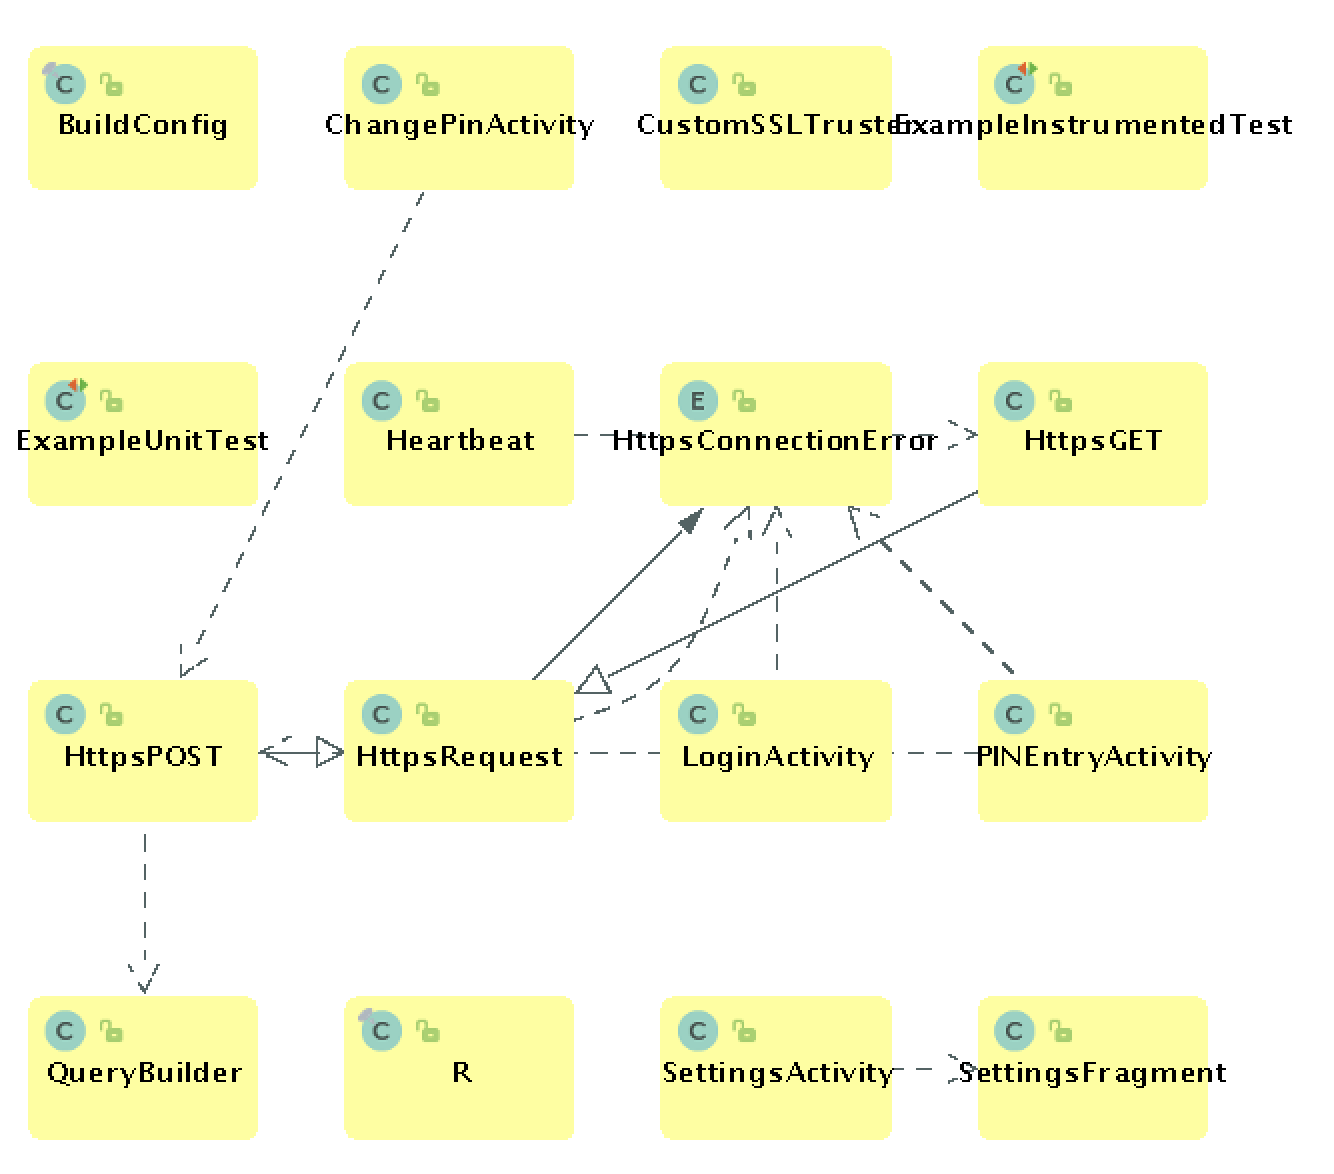
\includegraphics[width=\textwidth,height=\textheight,keepaspectratio]{Class_diagram_0_1_0.png}
	\caption{Συνοπτικό διάγραμμα κλάσεων για την έκδοση 0.1.0}
	\end{figure}

	\begin{figure}[p]
	\centering
		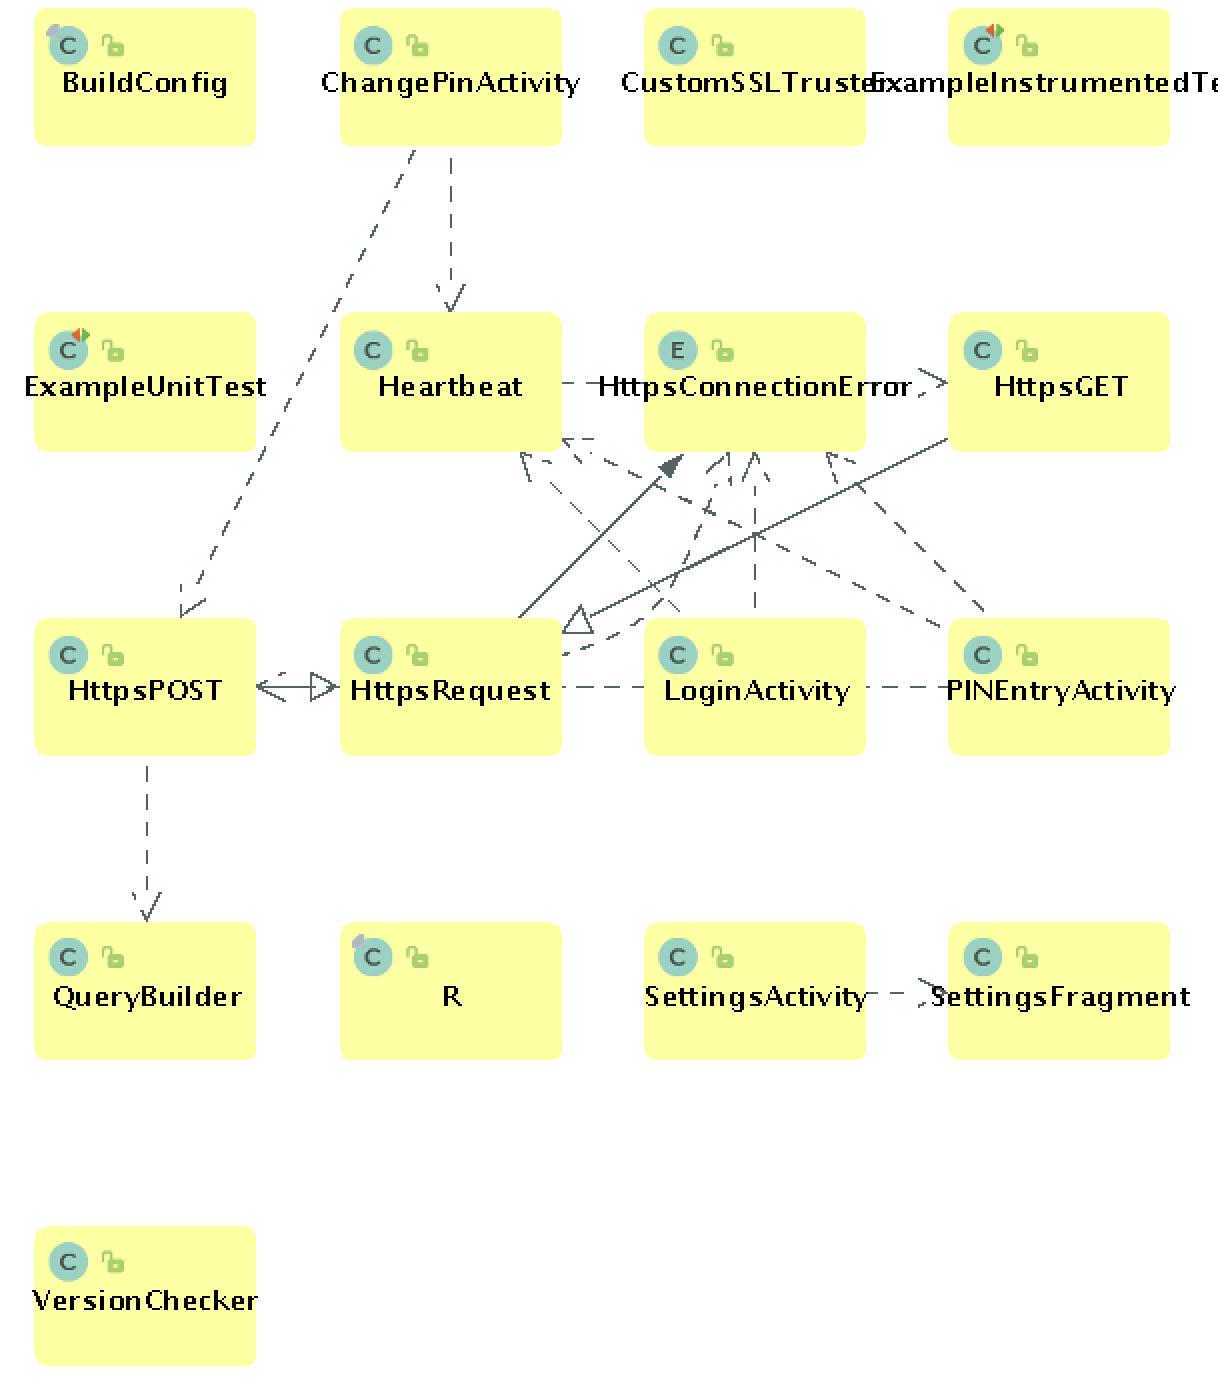
\includegraphics[width=\textwidth,height=\textheight,keepaspectratio]{Class_diagram_0_2_0.png}
	\caption{Συνοπτικό διάγραμμα κλάσεων για την έκδοση 0.2.0}
	\end{figure}

	\begin{figure}[p]
	\centering
		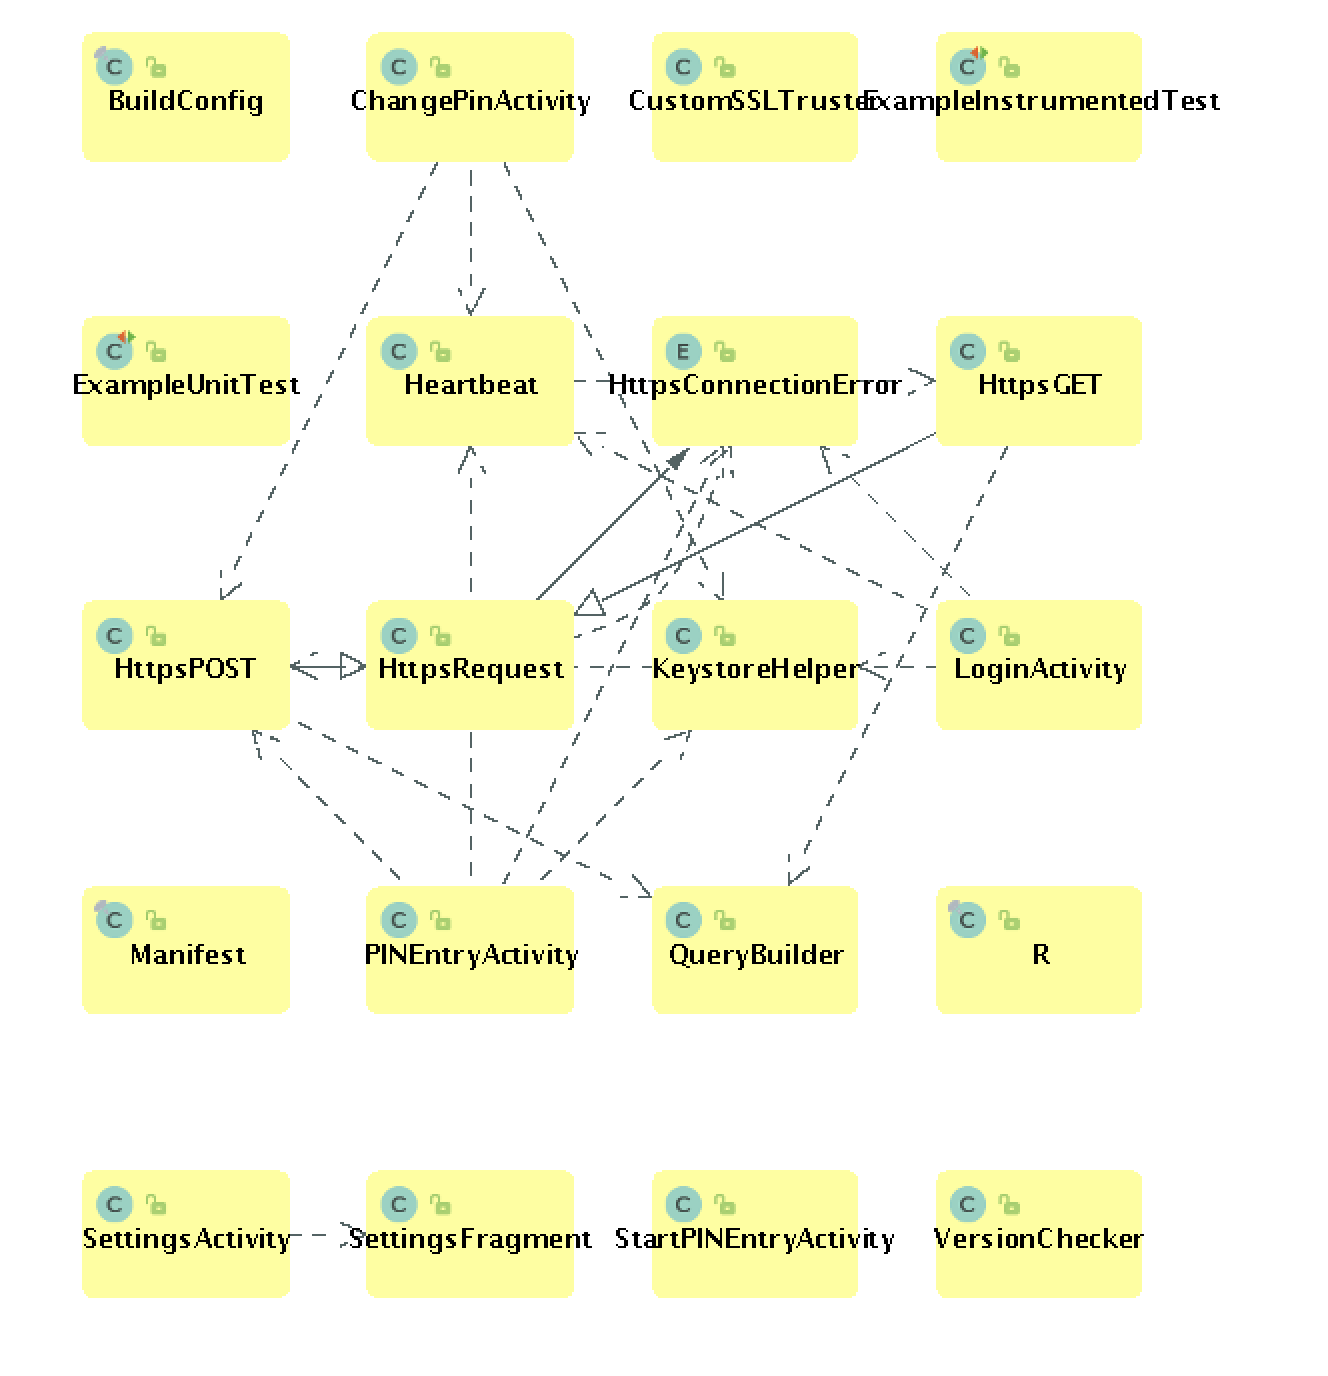
\includegraphics[width=\textwidth,height=\textheight,keepaspectratio]{Class_diagram_0_3_1.png}
	\caption{Συνοπτικό διάγραμμα κλάσεων για την έκδοση 0.3.0}
	\end{figure}

	\begin{figure}[p]
	\centering
		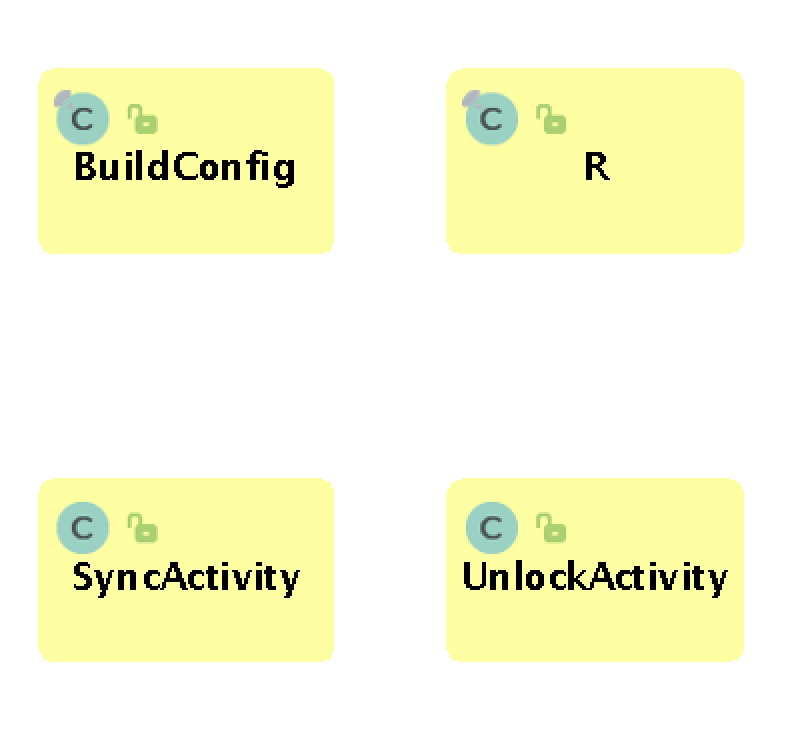
\includegraphics[width=\textwidth,height=\textheight,keepaspectratio]{Class_diagram_wear.png}
	\caption{Συνοπτικό διάγραμμα κλάσεων για την έκδοση για Android Wear}
	\end{figure}
\newpage
\section{Διαγράμματα Περιπτώσεων Χρήσεων Εκδόσεων}
	\label{ap:version_usecase_diag}
	\begin{figure}[h]
	\centering
		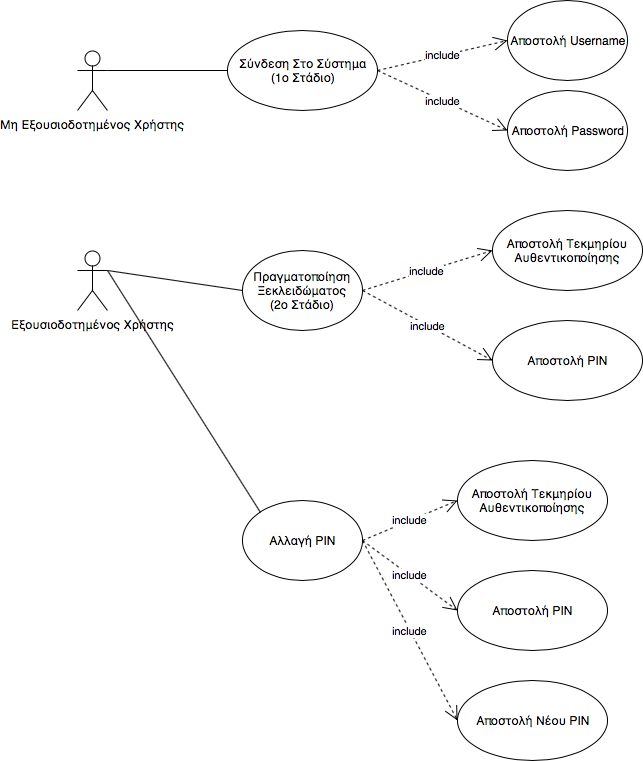
\includegraphics[width=\textwidth,height=\textheight,keepaspectratio]{0_1_0UseCase.png}
	\caption{Διάγραμμα Περιπτώσεων Χρήσης για την έκδοση 0.1.0}
	\end{figure}

	\begin{figure}[p]
	\centering
		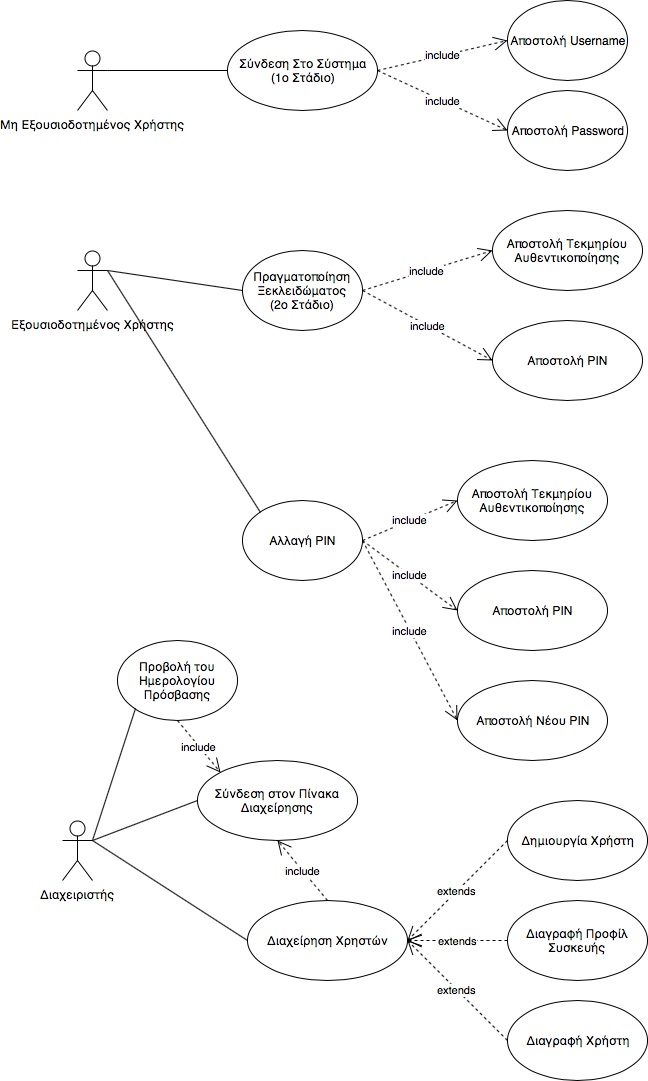
\includegraphics[width=0.75\textwidth,height=\textheight,keepaspectratio]{0_2_0UseCase.png}
	\caption{Διάγραμμα Περιπτώσεων Χρήσης για την έκδοση 0.2.0}
	\end{figure}

	\begin{figure}[p]
	\centering
		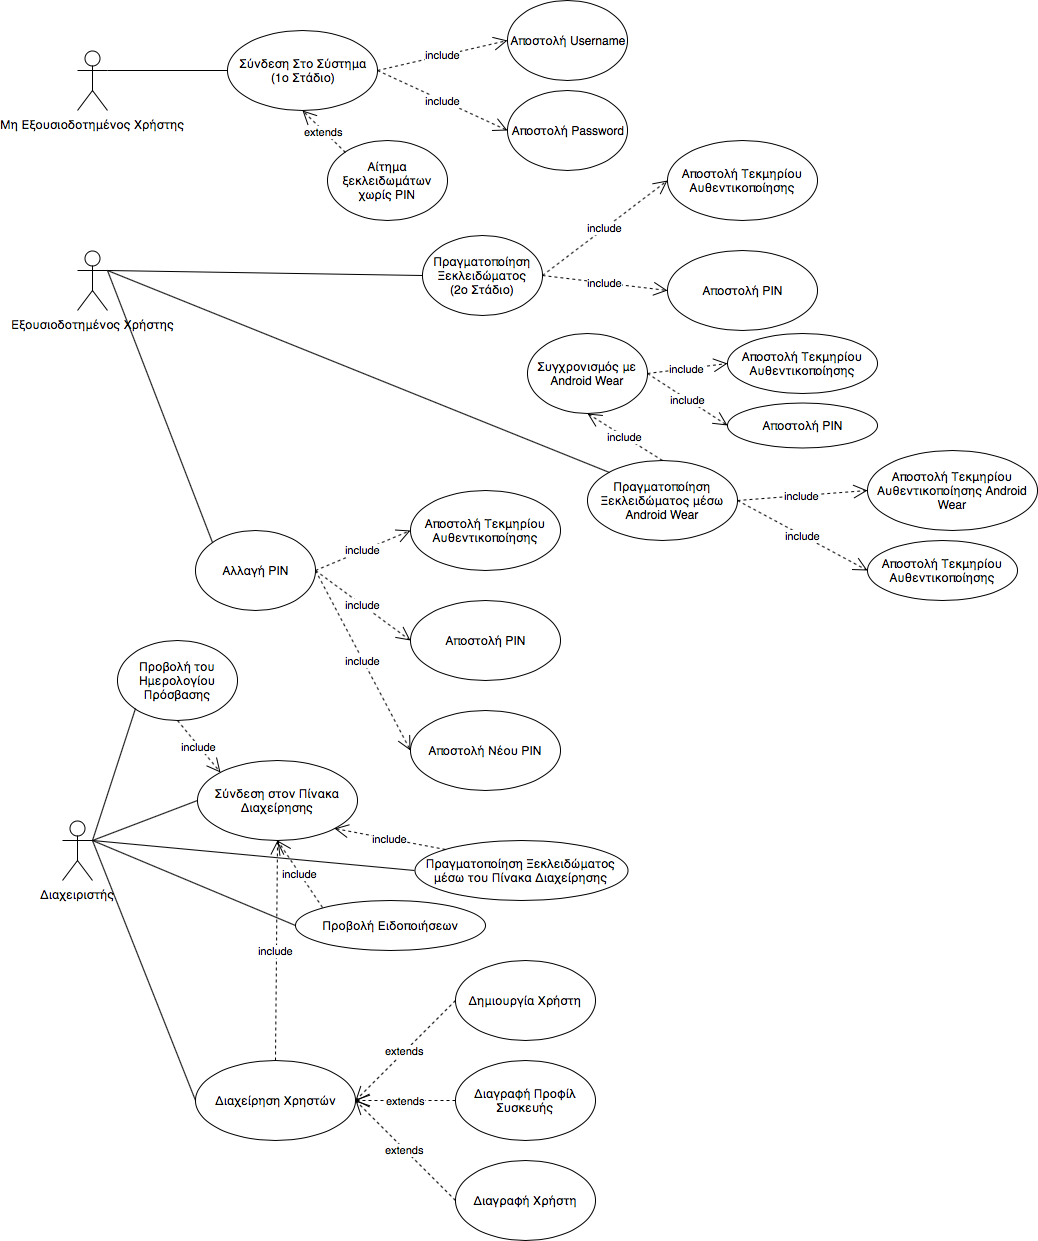
\includegraphics[width=\textwidth,height=\textheight,keepaspectratio]{0_3_0UseCase.png}
	\caption{Διάγραμμα Περιπτώσεων Χρήσης για την έκδοση 0.3.0}
	\end{figure}

    \begin{thebibliography}{99}

\bibitem{iotterm}
Kevin Ashton (2009), "That 'Internet of Things' thing"\\
\url{http://www.rfidjournal.com/articles/view?4986}

\bibitem{domotics}
Jim Hill (2015), "The smart home: a glossary guide for the perplexed"\\
\url{https://www.t3.com/features/the-smart-home-guide}

\bibitem{rpizw}
Ian Paul (2017), "The \$10 Raspberry Pi Zero W brings Wi-Fi and Bluetooth to the minuscule micro-PC"\\
\url{https://www.pcworld.com/article/3175256/computers/the-10-raspberry-pi-zero-w-brings-wi-fi-and-bluetooth-to-the-minusule-micro-pc.html}

\bibitem{rpizspecs}
Eben Upton (2015), "RASPBERRY PI ZERO: THE \$5 COMPUTER"\\
\url{https://www.raspberrypi.org/blog/raspberry-pi-zero/}

\bibitem{relay_purpose}
Relay, Wikipedia\\
\url{https://en.wikipedia.org/wiki/Relay}

\bibitem{arduino_definition}
Arduino for Beginners, Makerspaces.com\\
\url{https://www.makerspaces.com/arduino-uno-tutorial-beginners/}

\bibitem{jumper_wires}
Jump Wire Structure (2003), Katayama Tatsuo\\
\url{http://www.freepatentsonline.com/6899560.html}

\bibitem{rpi_wifi_headless}
How to connect raspberry pi to WiFi without a monitor (2017), Chetan Kapoor\\
\url{https://installvirtual.com/how-to-connect-raspberry-pi-to-wifi-without-a-monitor/}

\bibitem{raspbian_nov2016_upd}
A security update for Raspbian PIXEL (2016), Simon Long\\ 
\url{https://www.raspberrypi.org/blog/a-security-update-for-raspbian-pixel/}

\bibitem{default_creds}
\url{https://www.raspberrypi.org/documentation/linux/usage/users.md}

\bibitem{secure_passwords}
How to Create a Secure Password You Can Remember Later: 4 Key Methods (2014), Kevan Lee\\
\url{https://open.buffer.com/creating-a-secure-password/}

\bibitem{raspbian_update}
Updating and Upgrading Raspbian
\url{https://www.raspberrypi.org/documentation/raspbian/updating.md}

\bibitem{find_rpi_ip}
\url{https://www.raspberrypi.org/documentation/remote-access/ip-address.md}

\end{thebibliography}

    \printindex
    
\end{document}